\documentclass[a4paper]{article}

\usepackage{NotesPackage2}
\usepackage[toc]{appendix}
\usepackage{biblatex}
\usepackage{subcaption}
\usepackage{xcolor, colortbl}
\usepackage{hyperref}

\addbibresource{bibliography/bibliography.tex}

% Sets
\newcommand{\st}{\mid}
\newcommand{\union}{\cup}
\newcommand{\intersection}{\cap}
\newcommand{\bigunion}{\bigcup}
\newcommand{\bigintersection}{\bigcap}
% Logic
\newcommand{\conjunction}{\wedge}
\newcommand{\disjunction}{\vee}
\DeclareMathOperator{\andOperator}{and}
\DeclareMathOperator{\orOperator}{or}
\newcommand{\logicalAnd}{\mathbin{\andOperator}}
\newcommand{\logicalOr}{\mathbin{\orOperator}}
% Perms and combs
\newcommand{\perms}[2]{\tensor[_{#1}]{P}{_{#2}}}
\newcommand{\combs}[2]{\tensor[_{#1}]{C}{_{#2}}}
% Variance and covariance as functions
\DeclareMathOperator{\Var}{Var}
\DeclareMathOperator{\Cov}{Cov}
% Other
\newcommand{\notesVersion}{1.0}
\newcommand{\notesDate}{23/12/2020}
\newcommand{\convolution}{\mathbin{*}}
\newcommand{\distributed}{\sim}
\newcommand{\normal}{\mathcal{N}}
\newcommand{\binomial}{\mathcal{B}}
\newcommand{\poisson}{\mathrm{Pois}}
\newcommand{\spinUp}{\uparrow}
\newcommand{\spinDown}{\downarrow}

\author{Willoughby Seago}
\date{September 21, 2020} 
\title{Statistics}

\makeglossaries
% Add glossary entries here
\newacronym{pdf}{PDF}{probability density function}
\newacronym{cdf}{CDF}{cumulative density function}
\newacronym{qm}{QM}{quantum mechanics}
\newacronym{rms}{RMS}{root-mean-square}
\newacronym{fwhm}{FWHM}{full width at half maximum}

\includeonly{weeks/week1, weeks/week2, weeks/week3}

\begin{document}
    \pagenumbering{roman}  % Number contents pages and glossaries with roman numerals
    \maketitle
    These are my notes for the statistics half of the Fourier analysis and statistics course from the University of Edinburgh as part of the third year of the theoretical physics degree.
    When I took this course in the 2020/21 academic year it was taught by Professor Andy Lawrence\footnote{\url{https://www.ph.ed.ac.uk/people/andy-lawrence}}.
    These notes are based on the lectures delivered as part of this course and the notes provided as part of this course.
    The content within is correct to the best of my knowledge but if you find a mistake or just disagree with something or think it could be improved please let me know.
    
    These notes were produced using \LaTeX\footnote{\url{https://www.latex-project.org/}}.
    Graphs where plotted using Matplotlib\footnote{\url{https://matplotlib.org/}}, NumPy\footnote{\url{https://numpy.org/}}, and SciPy\footnote{\url{https://scipy.org/scipylib/}}.
    Diagrams were drawn with tikz\footnote{\url{https://www.ctan.org/pkg/pgf}}.
    
    This is version \notesVersion~of these notes, which is up to date as of \notesDate.
    \begin{flushright}
        Willoughby Seago
        
        s1824487@ed.ac.uk
    \end{flushright}
    \clearpage
    \tableofcontents
    \listoffigures
    \listoftables
    \printglossary[type=\acronymtype, title=Acronyms, style=long]
    \clearpage
    \pagenumbering{arabic}  % Number rest of document with numbers
    \begingroup
        \let\clearpage\relax  % "\begingroup, \let\clearpage\relax, \endgroup" stops automatic pagebreaks after each include
        
    \section{Course Overview}
    \subsection{Why is Statistics Useful?}
    Physics is about reasoning about the world using our knowledge, logic, and experiments.
    Statistics is about reasoning with incomplete knowledge.
    This is a common situation for reasons we will get to later.
    Using statistics we can still make statements about certain scenarios even if we can't know something for sure.
    
    For example we will play a game.
    We have a 6 sided die (a d6) and we roll it.
    I ask you to predict the result.
    If you get it right I give you \pounds1 and if you get it wrong you give me \pounds 1.
    Is this a good bet?
    If not why not?
    We immediately know that this is a bad bet.
    If asked why we may say something like `5 times out of 6 we are going to loose and only 1 time out of 6 will we win, therefore we will lose more than we gain'.
    What if we change the amounts so instead if you are correct you get \pounds6?
    Is this now a good bet?
    It turns out it is.
    The logic is similar to before but now the possible reward has increased we actually expect to win more money than we loose even though we expect to loose more games than we win.
    Statistics and probability allow us to take scenarios like this one, and much more complicated ones, and treat them rigorously to see what we expect as an outcome.
    
    \subsection{Course Structure}
    This course is divided into 3 parts:
    \begin{enumerate}[label=\Alph*.]
        \item Basics of probability -- What is probability?
        How do we do calculations with probability?
        How do we deal with probability distributions?
        
        \item Forward logic -- Given a set up what is the probability of a given result?
        For example what is the probability that upon rolling two dice one of them gives a 6?
        What is the probability that the sum is 9?
        What is the probability that the sum is more than 5?
        
        \item Backwards logic -- Given a result what can we say about the initial set up?
        For example given results from an experiment what function can we fit to the data?
        How good is this fit?
    \end{enumerate}
    
    \subsection{Is Anything Really Random?}
    Rolling a die is a quintessential example of randomness.
    But is it truly random?
    If we know enough information about the die, for example the velocity, angular velocity, and mass of the die, as well as environmental information like the surface it is being rolled on, the viscosity of the air, etc. then in theory we could compute which face will end up on top.
    In this sense rolling dice is not \emph{truly} random.
    We say that the process of rolling dice is deterministic in that with enough information we know the outcome.
    However in practice we almost always lack the required knowledge to make this calculation so we have to treat the result of a dice roll as if it were a random event.
    
    It is also possible that not all observers have the same information.
    If I take a coin and place it in one of my hands behind my back I know where the coin is.
    The best that you can do is guess, with a \SI{50}{\percent} chance of being correct.
    In this way we see that probability is subjective in that it depends on the observer.
    
    Often all observers are in the same boat.
    Consider a mole of gas (so on the order of \(\num{e23}\) molecules).
    In principle this system is (classically) deterministic.
    Say we want to know what the velocity of a certain particle will be after some time.
    We could, in theory, start with enough information to work this out.
    However there is no practical way to do this.
    If we start with the velocity of every particle, so 3 numbers for the 3 directions, stored as 32 bit floats (the standard size for a float in C) then we have \(3\cdot 32\cdot\num{e23} = \num{e25}\) bits of information.
    That is \(\num{e9}\) petabytes.
    One petabyte of storage costs approximately half a million dollars.
    Therefore just storing the velocities of all particles costs \$500 trillion, which is about six times the world GDP.
    Clearly there is \emph{no} way that this calculation can be done by anyone.
    However we could imagine some god-like entity that \emph{could} perform this calculation so the system is still deterministic.
    It is just that the best that we can do is treat this system statistically.
    
    The final form of randomness that we will consider is \acrfull{qm}.
    In many interpretations of \acrshort{qm} there are processes that are truly random.
    For example if we have maximum information about an electron, including its spin about the \(z\)-axis, and we measure its spin about the \(x\)-axis then there is still a 50/50 chance that we measure spin up/down in that direction.
    There is no way to know before the measurement what the result will be.
    In this way \acrshort{qm} provides us with true randomness.
    However there are interpretations of \acrshort{qm} where things are deterministic and the randomness is again just missing information.
    
    We see that there are three possible levels of randomness:
    \begin{enumerate}
        \item Random for at least one observers perspective due to missing information.
        \item Random from all reasonable observers perspectives due to impracticality of computations even with perfect knowledge.
        \item Random from all observers perspectives even with perfect knowledge due to random quantum effects.
    \end{enumerate}
    All three types of randomness can be treated with statistics and probability.

    \section{Probability Basics}
    There are two ways to view probability:
    \begin{itemize}
        \item The probability of an event is the frequency with which it will occur if we are given the same starting scenario multiple times.
        This is called the frequentist approach.
        \item The probability of an event is a measure of how confident we are that that event will occur.
        This is called the Bayesian approach.
    \end{itemize}
    These two approaches are different ways of thinking but are equivalent and can be combined as long as we are careful.
    We will start by looking at the frequentist view.
    
    \subsection{Random Variables}
    To start with we will look at a random variable.
    For our purposes a sufficient definition of a random variable is a variable that has a value dependent on some random process.
    This process may be truly random or we may simply lack information required to know its value.
    Random variables can be discrete or continuous.
    It is common to use capital letters, such as \(X\), for discrete random variables and lowercase letters, such as \(x\), for continuous random variables.
    
    \subsubsection{Discrete Probability}
    Consider a discrete random variable, \(X\).
    For example \(X\) could be the value of rolling a die.
    The set \(S = \{X_i\st i\in I\}\) is called the sample space.
    It is the set of all possible outcomes, \(X_i\).
    Here \(I\) is some indexing set.
    It could be finite, such as \(I = \{1, \dotsc, 6\}\) for rolling a d6, or countably infinite, such as a process that could give any integer value where we may have \(I = \integers\).
    Starting with the same set up perform \(N\) measurements of \(X\).
    Let \(N_i\) be the number of times that we measure \(X_i\) as the value of \(X\).
    We define the probability that we measure \(X\) to be \(X_i\) to be 
    \[P_i = P(X = X_i) = P(X_i) = \lim_{N\to\infty} \frac{N_i}{N}.\]
    Here \(P_i\), \(P(X = X_i)\), and \(P(X_i)\) are just different ways to notate `the probability that we measure \(X\) to take the value \(X_i\)'.
    From the definition of \(N_i\) it is clear that
    \[\sum_{i\in I} N_i = N\]
    and therefore
    \[\sum_{i\in I} P_i = \frac{1}{N}\sum_{i\in I}N_i = \frac{N}{N} = 1.\]
    In this way we think of \(P_i\) as the normalised frequency of measuring \(X\) to have the value \(X_i\).
    
    Going back to our example of rolling a d6 we have \(S = \{1, \dotsc, 6\}\) and all probabilities are equally likely.
    Therefore we have
    \[P(X = X_i) = \frac{1}{6}.\]
    To do this calculation we used that each \(X_i\in S\) is equally likely and the total probability has to be 1.
    All being equally likely means that \(P_i = 1/|S| = 1/6\).
    We could ask a slightly more complicated question such as what is the probability that we get an even number.
    The frequentist way to answer this is to find out how many of the possible outcomes are even and collect them in a set, \(E = \{2, 4, 6\}\).
    Thus there are 3 ways to get an even number out of 6 possible results and all results are equally likely.
    Therefore
    \[P(E) = \frac{|E|}{|S|} = \frac{3}{6} = \frac{1}{2} = 0.5,\]
    which is what we would expect.
    
    We can ask a more complicated question such as what happens if we roll 2 d6?
    The sample space is now
    \[S = \{(X_i, Y_i)\st X_i, Y_i\in\{1, \dotsc, 6\}\}.\]
    We now have \(|S| = 36\).
    All possible results are still equally likely as long as we treat \((X_i, Y_i)\) as different to \((Y_i, X_i)\).
    Therefore we have \(P((X_i, Y_i)) = 1/36\) for some specific \((X_i, Y_i)\in S\).
    We now ask questions about the sum \(T((X_i, Y_i)) = X_i + Y_i\).
    For ease we list all possible values of \(X_i\) and \(Y_i\) and the sum \(T\) in table~\ref{tab:possible values of T = sum of 2 d6}.
    \begin{table}[ht]
        \centering
        \[
            \begin{array}{cc}
                & Y_i\\
                X_i &
                \begin{array}{c|cccccc}
                       & 1 & 2 & 3 & 4 & 5 & 6\\\hline
                     1 & 2 & 3 & 4 & 5 & 6 & 7\\
                     2 & 3 & 4 & 5 & 6 & 7 & 8\\
                     3 & 4 & 5 & 6 & 7 & 8 & 9\\
                     4 & 5 & 6 & 7 & 8 & 9 & 10\\
                     5 & 6 & 7 & 8 & 9 & 10 & 11\\
                     6 & 7 & 8 & 9 & 10 & 11 & 12
                \end{array}
            \end{array}
        \]
        \caption{Possible values of \(T = X_i + Y_i\) for \(X_i\) and \(Y_i\) being the result of rolling a d6.}
        \label{tab:possible values of T = sum of 2 d6}
    \end{table}
    We can treat \(T\) as a random variable.
    Say we want to know what the probability is that \(T = 5\).
    There are 36 possible pairs \((X_i, Y_i)\) and of these we see from the table that 4 of them sum to \(5\).
    Thus
    \[P(T = 5) = \frac{4}{36} = \frac{1}{9} = 0.\bar{1}.\]
    We can do this for all possible values of \(T\).
    If we do then we can list the results in another table:
    \[
        \begin{array}{c|cccccccccccccc}
            T & 0 & 1 & 2 & 3 & 4 & 5 & 6 & 7 & 8 & 9 & 10 & 11 & 12 & 13\\\hline
            N_T & 0 & 0 & 1 & 2 & 3 & 4 & 5 & 6 & 5 & 4 & 3 & 2 & 1 & 0
        \end{array}
    \]
    We can define a discrete \acrfull{pdf}, \(p\colon S_T \rightarrow [0, 1]\) where \(S_T\) is the sample space of possible values of \(T\).
    We define \(p(T_i) = P(T = T_i)\) for \(T_i \in S_T\) and \(p(T_i) = 0\) for \(T_i\notin S_T\).
    We can plot \(p\) to get a graphical representation of the various probabilities from which we can easily read off values for specific \(T_i\).
    This is what we have done in figure~\ref{fig:2d6 pdf}
    \begin{figure}[ht]
        \centering
        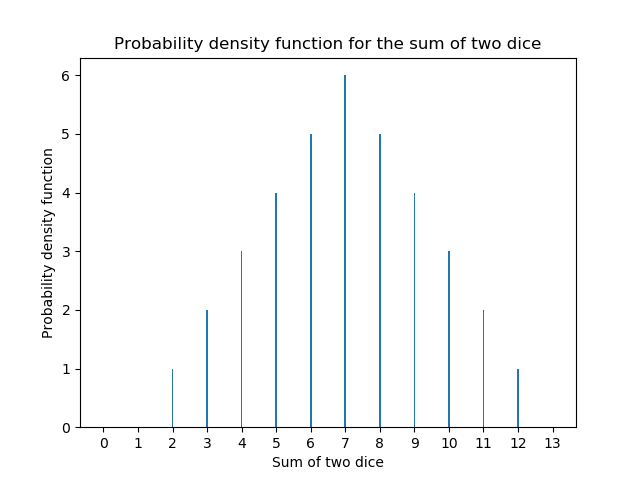
\includegraphics[scale=0.6]{pdf_2d6.png}
        \caption{Probability density function for the sum of two six sided dice.}
        \label{fig:2d6 pdf}
    \end{figure}
    
    \subsubsection{Continuous Probability}
    Consider a continuous random variable, \(x\).
    For example \(x\) could be the speed of a molecule in a gas.
    Again we can define a sample space \(S = \{x_i\st i\in I\}\), which is the set of all possible values for \(x\).
    Here \(I\) is an indexing set that is now uncountably infinite.
    With our example of the speed of a molecule we would expect \(S = [0, \infty)\).
    In order for probabilities to sum to 1 it is necessary that \(P(x_i) = 0\) for all \(x_i \in S\).
    Instead we can only meaningfully talk about the probability that \(x\) is in a given range.
    We define a continuous probability density function, \(p\colon S\rightarrow [0, 1]\), so that \(p(x)\dd x\) is the probability of measuring a value to be in \([x, x + \dd x]\) for some infinitesimal \(\dd x\).
    An example of a continuous \acrshort{pdf} is given in figure~\ref{fig:example continuous pdf}.
    \begin{figure}[ht]
        \centering
        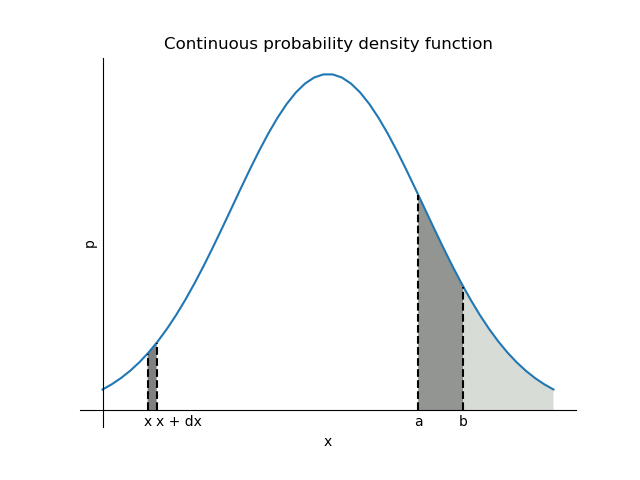
\includegraphics[scale=0.6]{example_continuous_pdf.png}
        \caption{A continuous \acrshort{pdf}.}
        \label{fig:example continuous pdf}
    \end{figure}
    Using this \acrshort{pdf} we can calculate different probabilities.
    The probability of measuring \(x\) to be in \([a, b]\) is
    \[\int_a^b p(x)\,\dd x\]
    and the probability of measuring \(x\) to be greater than \(b\) is
    \[\int_b^\infty p(x)\,\dd x.\]
    This should be enough to calculate all probabilities of interest.
    
    \subsection{Calculating the Probability of \texorpdfstring{\(A\logicalAnd B\)}{A and B}}
    Independent events have no effect on each others probabilities.
    Examples of independent events are
    \begin{itemize}
        \item The values rolled on two different dice.
        \item Selecting cards with replacement.
        \item Whether it is raining and the value of the pound.
    \end{itemize}
    Dependent events are then events which do effect the outcome of each other.
    Examples of dependent events are
    \begin{itemize}
        \item Whether an integer is prime and whether that number is odd.
        \item Selecting cards without replacement.
        \item Whether it is raining and the number of umbrellas in use.
    \end{itemize}
    
    Let \(A\) and \(B\) be two different events.
    We wish to know the probability that both \(A\) and \(B\) occur.
    We denote this \(P(A\logicalAnd B)\) or \(P(A, B)\).
    Viewing \(A\) and \(B\) as sets of possible outcomes we may also write it as \(A\intersection B\).
    Viewing \(A\) and \(B\) as hypotheses (as we will do later) we may write it as \(A\conjunction B\).
    We will start with an example.
    
    Take the following 6 cards from a deck: \(J\diamondsuit\), \(Q\diamondsuit\), \(K\diamondsuit\), \(J\clubsuit\), \(Q\clubsuit\), and \(K\clubsuit\).
    Separate the cards into the two suits and shuffle each triplet of cards.
    From each triplet select one card.
    What is the probability of getting 2 kings?
    First note that the two cards we get are independent events.
    The possible pairs are best described in the following table, with the number of kings in the pair listed:
    \[
        \begin{array}{c|ccc}
            & J\clubsuit & Q\clubsuit & K\clubsuit\\\hline
            J\diamondsuit & 0 & 0 & 1\\
            Q\diamondsuit & 0 & 0 & 1\\
            K\diamondsuit & 1 & 1 & 2
        \end{array}
    \]
    We see that there are 9 possible pairs \((X\diamondsuit, Y\clubsuit)\) where \(X, Y\in \{J, Q, K\}\).
    Of these only one pair has two kings, \((K\diamondsuit, K\clubsuit)\).
    Therefore the probability of getting two kings is
    \[P(\text{2 kings}) = P(K\diamondsuit \logicalAnd K\clubsuit) = \frac{1}{9} = 0.\bar{1}.\]
    Note that this is the same as
    \[P(K\diamondsuit)P(K\clubsuit) = \frac{1}{3}\cdot\frac{1}{3} = \frac{1}{9} = 0.\bar{1}.\]
    What if instead we shuffled all 6 cards together and then picked two cards without replacement?
    The first time we pick a card there are 6 cards and 2 of them are kings so the probability that we get a king is
    \[P(\text{first card is a king}) = \frac{2}{6} = \frac{1}{3} = 0.\bar{3}.\]
    The second time we pick a card there are 5 cards but the number of kings depends on what we picked the first time.
    Since we want two kings we assume that the first time we picked a king (if we didn't there would be no way to get 2 kings).
    Therefore there is 1 king left.
    We then calculate the probability of selecting a king given we have already picked a king.
    In general the probability of event \(B\) given that event \(A\) has occurred is \(P(B|A)\).
    The probability that we get a king the second time given we got a king the first time is
    \[P(\text{second card is a king}|\text{first card is a king}) = \frac{1}{5} = 0.2.\]
    We can now calculate the probability that we select two kings:
    \[P(\text{2 kings}) = P(\text{first card is a king})P(\text{second card is a king}|\text{first card is a king}) = \frac{1}{3}\cdot\frac{1}{5} = \frac{1}{15} = 0.0\bar{6}.\]
    
    In general we find that for two events \(A\) and \(B\) the probability that both occur is
    \[P(A\logicalAnd B) = P(A)P(B|A).\]
    Note that if \(A\) and \(B\) are independent then \(B\) is equally likely to occur whether or not \(A\) occurs so \(P(B|A)\) reduces to \(P(B)\).
    Therefore this formula works regardless of whether \(A\) and \(B\) are independent.
    
    We can view \(A\) and \(B\) as sets of possible outcomes.
    In this case
    \[P(A) = \frac{|A|}{|S|},\qquad\text{and}\qquad P(B) = \frac{|B|}{|S|}\]
    where \(S\) is the sample space.
    We can view the possible outcomes visually in figure~\ref{fig:venn diagram for events A and B}.
    \begin{figure}[ht]
        \centering
        \begin{tikzpicture}
            \draw (0, 0) rectangle (10, 5);
            \node at (0.5, 4.5) {\(S\)};
            \begin{scope}
                \clip (3.5, 2.5) circle[radius=2.2cm];
                \clip (6.5, 2.5) circle[radius=2.2cm];
                \draw[fill=lightgray] (0, 0) rectangle (10, 5);
            \end{scope}
            \draw (3.5, 2.5) circle[radius=2.2cm];
            \draw (6.5, 2.5) circle[radius=2.2cm];
            \node at (3.5, 2.5) {\(A\)};
            \node at (6.5, 2.5) {\(B\)};
            \node at (5, 2.5) {\(A\intersection B\)};
            \node at (5.5, -0.5) {\( = A\intersection B\)};
            \draw[fill=lightgray, color=lightgray] (4.5, -0.7) rectangle (4.8, -0.3);
        \end{tikzpicture}
        \caption{Venn diagram for events \(A\) and \(B\)}
        \label{fig:venn diagram for events A and B}
    \end{figure}
    In this figure the shaded area represents the outcomes that are in \(A\) and \(B\), this is the intersection, \(A\intersection B\), of the sets \(A\) and \(B\).
    Like any probability viewed as sets we calculate the probability as
    \[P(A\logicalAnd B) = P(A\intersection B) = \frac{|A\intersection B|}{|S|}.\]
    
    Note that `\(\logicalAnd\)' is symmetric.
    That is \(P(A\logicalAnd B) = P(B\logicalAnd A)\).
    This means that
    \[P(A\logicalAnd B) = P(A)P(B|A) = P(B)P(A|B) = P(B\logicalAnd A).\]
    Rearranging this we get
    \[P(B|A) = \frac{P(A|B)P(B)}{P(A)}.\]
    This is known as Bayes' theorem and it turns out to be very important in Bayesian statistics.
    
    \subsection{Calculating the Probability of \texorpdfstring{\(A \logicalOr B\)}{A or B}}
    Mutually exclusive events cannot both occur at the same time.
    For example getting heads and tails are mutually exclusive.
    On the other hand a number being even and a prime is possible so even and prime are not mutually exclusive.
    If two events, \(A\) and \(B\), are mutually exclusive then \(P(A\logicalAnd B) = 0\), or in terms of sets \(A\intersection B = \emptyset\).
    We can represent mutually exclusive events graphically, as we have in figure~\ref{fig:mutually exclusive events}.
    We see that \(A\intersection B = \emptyset\) so \(|A\intersection B| = 0\).
    Since there is no overlap between the two sets the size of the union is the sum of the size of the two sets:
    \[|A\union B| = |A| + |B|.\]
    Therefore the probability of \(A \logicalOr B\) is
    \[P(A\logicalOr B) = \frac{|A| + |B|}{|S|} = P(A) + P(B).\]
    \begin{figure}[ht]
        \centering
        \begin{tikzpicture}
            \draw (0, 0) rectangle (10, 5);
            \node at (0.5, 4.5) {\(S\)};
            \begin{scope}
                \clip (3, 2.5) circle[radius=1.8cm];
                \draw[fill=lightgray] (0, 0) rectangle (10, 5);
            \end{scope}
            \begin{scope}
                \clip (7, 2.5) circle[radius=1.8cm];
                \draw[fill=lightgray] (0, 0) rectangle (10, 5);
            \end{scope}
            \draw (3, 2.5) circle[radius=1.8cm];
            \draw (7, 2.5) circle[radius=1.8cm];
            \node at (3, 2.5) {\(A\)};
            \node at (7, 2.5) {\(B\)};
            \node at (5.5, -0.5) {\( = A\union B\)};
            \draw[fill=lightgray, color=lightgray] (4.5, -0.7) rectangle (4.8, -0.3);
        \end{tikzpicture}
        \caption{Mutually exclusive events}
        \label{fig:mutually exclusive events}
    \end{figure}
    If instead we take \(A\) and \(B\) to not be mutually exclusive then we have a scenario more like figure~\ref{fig:not mutually exclusive events}.
    In this case we have \(A\intersection B \ne \emptyset\) so \(|A\intersection B| \ne 0\).
    Note that we say \(A\) and \(B\) are disjoint sets if \(A\intersection B = \emptyset\).
    We need to find \(|A\union B|\).
    We start with the naive answer of \(|A\union B| = |A| + |B|\) but we notice that this isn't quite right.
    Say \(x\in A\intersection B\) then \(x\) is counted in \(|A|\) and \(|B|\).
    We therefore count everything in \(A\intersection B\) twice.
    To remedy this we subtract the size of the intersection to get
    \[|A\union B| = |A| + |B| - |A\intersection B|.\]
    \begin{figure}[ht]
        \centering
        \begin{tikzpicture}
            \draw (0, 0) rectangle (10, 5);
            \node at (0.5, 4.5) {\(S\)};
            \begin{scope}
                \clip (3.5, 2.5) circle[radius=2.2cm];
                \draw[fill=lightgray] (0, 0) rectangle (10, 5);
            \end{scope}
            \begin{scope}
                \clip (6.5, 2.5) circle[radius=2.2cm];
                \draw[fill=lightgray] (0, 0) rectangle (10, 5);
            \end{scope}
            \draw (3.5, 2.5) circle[radius=2.2cm];
            \draw (6.5, 2.5) circle[radius=2.2cm];
            \node at (3.5, 2.5) {\(A\)};
            \node at (6.5, 2.5) {\(B\)};
            \node at (5, 2.5) {\(A\intersection B\)};
            \node at (5.5, -0.5) {\( = A\union B\)};
            \draw[fill=lightgray, color=lightgray] (4.5, -0.7) rectangle (4.8, -0.3);
        \end{tikzpicture}
        \caption{Not mutually exclusive events}
        \label{fig:not mutually exclusive events}
    \end{figure}
    This formula actually also works if \(A\) and \(B\) are disjoint as then \(A\intersection B = \emptyset\) so the final term is zero.
    Therefore this formula works regardless of whether or not \(A\) and \(B\) are mutually exclusive.
    The probability that event \(A\) or \(B\) or both occur is
    \[P(A\logicalOr B) = P(A\union B) = \frac{|A| + |B| - |A\intersection B|}{|S|} = P(A) + P(B) - P(A\logicalAnd B).\]
    
    \subsection{Probability as Degree of Belief}
    So far we have used a frequentist approach to probability.
    A Bayesian approach involves hypotheses.
    A hypothesis is a statement, \(H\), that is either true or false.
    We can assign to each hypothesis a number, \(C(H)\), representing its credibility.
    Let \(S = \{H_i\st i\in I\}\), where \(I\) is some indexing set that will be countable if \(H_i\) involves discrete variables, or uncountable if \(H_i\) involve continuous variables. \(S\) is the sample space, that is the set of all possible hypotheses. \(C\colon S \rightarrow [0, 1]\) is defined so that \(C(H)\) is the credibility of \(H\).
    It can be shown that there is a unique way to assign a credibility to  \(H_i\) if we require the following to hold:
    \begin{enumerate}
        \item \(C(H_1) > C(H_2)\) if we have a stronger belief in \(H_1\) than \(H_2\).
        \item \(\sum_i H_i = 1\).
        \item \(C(H_1\conjunction H_2) = C(H_1)C(H_2|H_1)\) where \(\conjunction\) represents the Boolean operator and.
        \item \(C(H_1\disjunction H_2) = C(H_1) + C(H_2) - C(H_1\conjunction H_2)\) where \(\disjunction\) represents the Boolean operator or.
    \end{enumerate}
    If we take these rules and identify \(C \leftrightarrow P\) and \(\conjunction/\disjunction\leftrightarrow \intersection/\union \leftrightarrow \text{and}/\text{or}\) then we recover the frequentist results.
        \section{Population Vs. Sample Distributions}
    We often assume the existence of a probability distribution for a given scenario.
    However the problem is we don't always know what this distribution is.
    One thing we can do to try and get a better understanding of it is to make measurements and look at the distribution of these measurements.
    The underlying probability distribution is called the population, or parent, distribution, and the distribution of the measurements is called the sample distribution.
    
    A simple example of this is tossing coins.
    Say we toss 4 coins, the population distribution tells us we should expect 2 heads.
    However this isn't guaranteed to happen every time.
    If we repeat this 4 coin toss 10 times we may get the following number of heads, \(X\):
    \[X = 4, 3, 2, 2, 2, 3, 1, 3, 1, 2.\]
    There is also a formula, 
    \[P_n(X) = \frac{n!}{X!(n - X)!}\left(\frac{1}{2}\right)^n,\]
    that gives the probability of getting \(X\) heads when you toss \(n\) coins.
    This is based on the binomial distribution which we will cover later.
    \begin{figure}[ht]
        \centering
        \begin{subfigure}{0.4\textwidth}
            \centering
            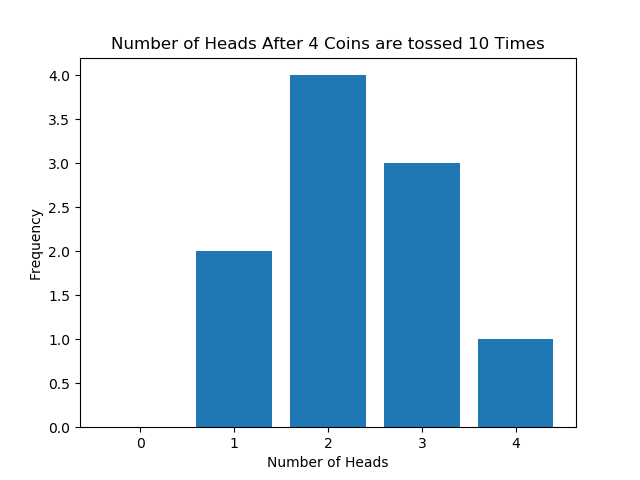
\includegraphics[scale=0.35]{coin_toss_results.png}
            \caption{Results of tossing 4 coins 10 times.}
            \label{fig:results of tossing 4 coins}
        \end{subfigure}
        \begin{subfigure}{0.4\textwidth}
            \centering
            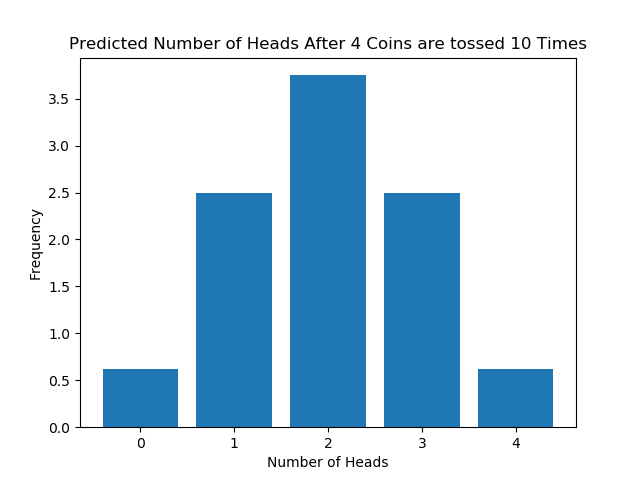
\includegraphics[scale=0.35]{coin_toss_prediction.png}
            \caption{Predicted number of heads for tossing 4 coins 10 times.}
            \label{fig:prediction of tossing 4 coins}
        \end{subfigure}
        \caption{Sample distribution vs. population distribution for counting the number of heads in four coin tosses.}
    \end{figure}
    The results of this experiment are plotted in figure~\ref{fig:results of tossing 4 coins} and the prediction is plotted in figure~\ref{fig:prediction of tossing 4 coins}.
    As you can see they are close but not quite the same.
    In general as we increase the number of times that we repeat an experiment we expect the results to look more and more like the prediction.
    We see this in figure~\ref{fig:10000 repeats} where the experiment was repeated 10000 times instead of 10 and the results and prediction are much closer.
    \begin{figure}[ht]
        \centering
        \begin{subfigure}{0.35\textwidth}
            \centering
            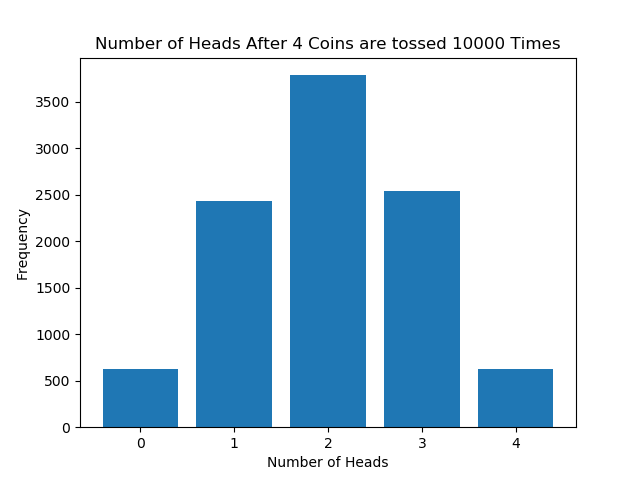
\includegraphics[scale=0.35]{coin_toss_results_10000.png}
            \caption{Results of tossing 4 coins 10 times.}
        \end{subfigure}
        \begin{subfigure}{0.35\textwidth}
            \centering
            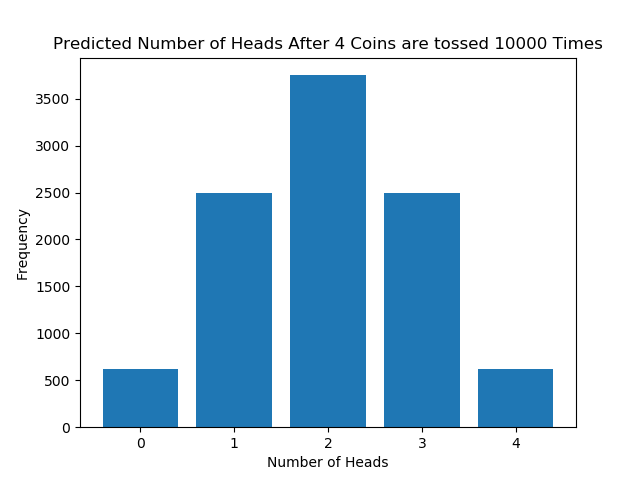
\includegraphics[scale=0.35]{coin_toss_prediction_10000.png}
            \caption{Predicted number of heads for tossing 4 coins 10 times.}
        \end{subfigure}
        \caption{Sample distribution vs. population distribution for counting the number of heads in four coin tosses.}
        \label{fig:10000 repeats}
    \end{figure}
    What we have here is that if \(f_n(X)\) is the number of times that \(X\) heads occurs in \(n\) coin tosses and \(N\) is the number of repeats then we expect
    \[\lim_{N\to\infty} \frac{f_n(X)}{N} = P_n(X).\]
    
    In the case of a continuous random variable, \(x\), then all of the above holds if we `bin' the results.
    By this we mean choose values, \(x_i\), of \(x\) and group the results into ranges around these values.
    This has been done in figure~\ref{fig:binned continuous sample}.
    \begin{figure}[ht]
        \centering
        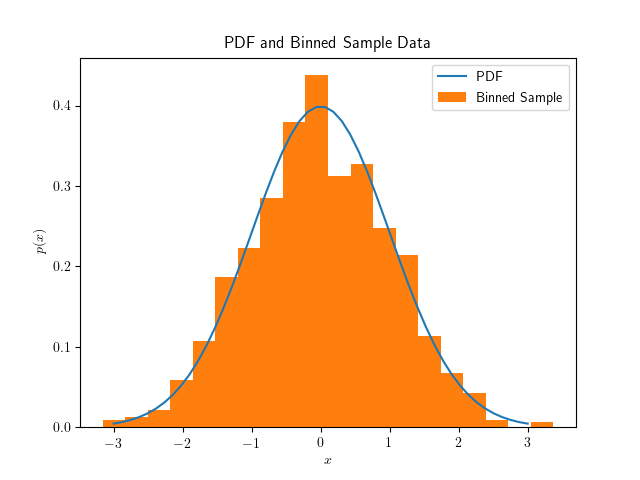
\includegraphics[scale=0.5]{binned_continuous_sample.png}
        \caption{A sample of a continuous random variable, binned, normalised, and plotted against the underlying \acrshort{pdf}.}
        \label{fig:binned continuous sample}
    \end{figure}
    Again we expect the normalised sample data to tend to the probability as we increase the number of repeats.
    If \(f(x_i)\) is the frequency with which data falls in the bin centred on \(x_i\), \(\Delta x\) is the width of the bin, and \(N\) is the size of the set of sample data then we expect
    \[\lim_{N\to\infty} \frac{f(x_i)}{N\Delta x} = p(x)\]
    
    \subsection{Multivariate Distributions}
    Often we have two random variables.
    If \(X\) and \(Y\) are discrete random variables then we can define a joint probability distribution, \(P\), by specifying \(P(X_i, Y_j)\) for all possible values of \(X_i\) and \(Y_j\).
    If instead \(x\) and \(y\) are continuous random variables then we define \(p(x, y)\) such that the probability that \((x, y)\in[x, x + \dd{x}]\times[y, y + \dd{y}]\) is \(p(x, y)\dd{x}\dd{y}\).
    
    Either way we end up with a three dimensional function (in the sense that we have two inputs and an output so need three dimensions to visualise it).
    We could use heat maps, contour maps, or 3D plots.
    \begin{figure}[ht]
        \centering
        \begin{subfigure}{0.35\textwidth}
            \centering
            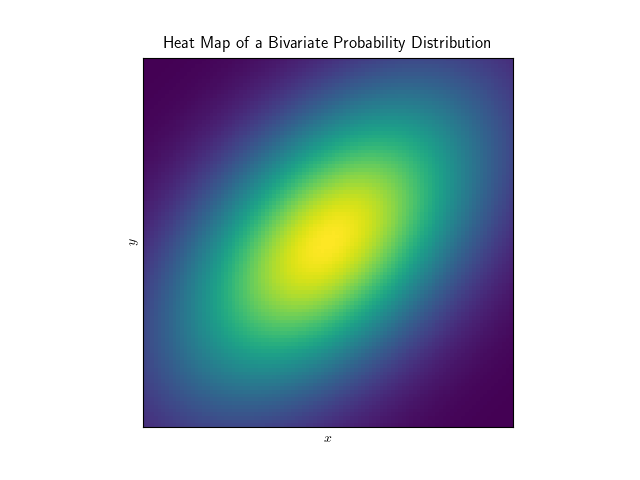
\includegraphics[scale=0.35]{bivariate_heat_map.png}
            \caption{A bivariate probability density function heat map.}
            \label{fig:bivariate heat map}
        \end{subfigure}
        \begin{subfigure}{0.35\textwidth}
            \centering
            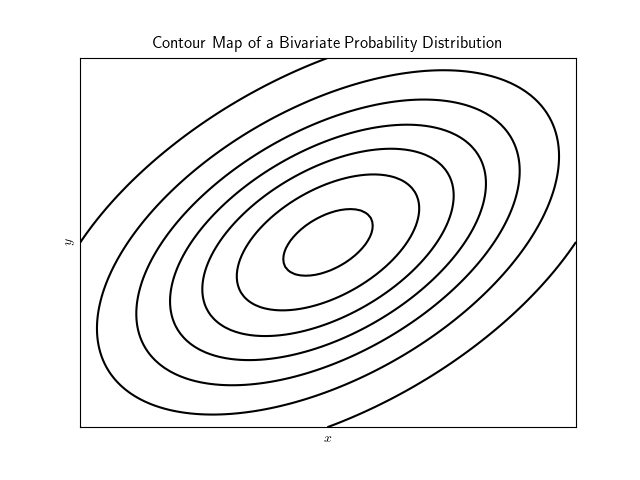
\includegraphics[scale=0.35]{bivariate_contour_map.png}
            \caption{A bivariate probability density function contour map.}
        \end{subfigure}
        \begin{subfigure}{0.35\textwidth}
            \centering
            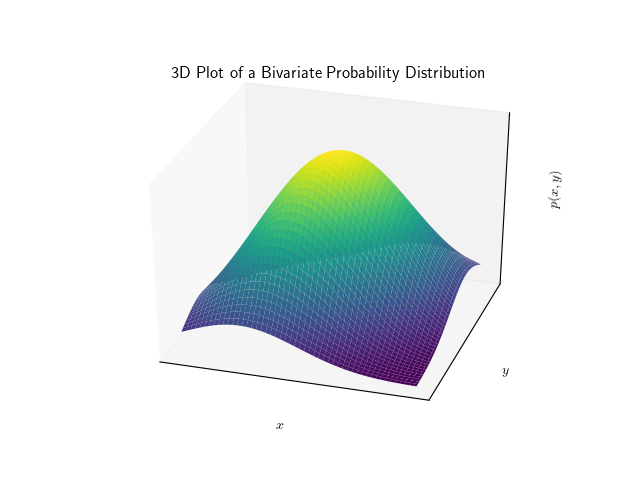
\includegraphics[scale=0.4]{bivariate_3d_plot.png}
            \caption{A bivariate probability density function plot.}
        \end{subfigure}
        \caption{Different ways to plot a bivariate probability distribution.}
    \end{figure}
    One question that we might logically ask is what information can we extract about one random variable from a joint probability distribution.
    The answer is that it depends what we want.
    If we want to know about one variable and have knowledge of the other then we get a different answer to if we want to know about one variable and don't care about the other.
    In the first case we get a conditional distribution and in the second a marginal distribution.
    
    \subsubsection{Conditional Distributions}
    If \((x, y)/(X, Y)\) is a pair of continuous/discrete random variables with probability density/probability given by \(p/P\) and we want information about \(x/X\) then one thing that we could do is fix \(y=y^*/Y=Y_j\) and look at \(p(x, y^*)/P(X, Y_j)\).
    This is like taking a slice through the data at this fixed value.
    We can define a new probability distribution/probability based off of this.
    In the continuous case we have
    \[q_{y^*}(x) = q(x|y^*) = \frac{p(x, y^*)}{\int p(x, y^*)\,\dd{x}}\]
    here the integral ensures that this is properly normalised.
    In the discrete case we have
    \[Q_j(X_i) = Q(X_i|Y_j) = \frac{P(X_i, Y_j)}{\sum_{j}P(X_i, Y_j)}.\]
    These are called conditional distributions because we are looking at distributions for \(x/X\) given a condition of some particular \(y/Y\) value.
    
    \begin{example}
        \begin{table}[ht]
            \centering
            \begin{tabular}{ccccccccc|c}
                &\multicolumn{8}{c}{Head Breadth/\si{\centi\metre}}&\\
                Head Length/\si{\centi\metre} & 13 & 13.5 & 14 & 14.5 & 15  & 15.5 & 16 & 16.5 & Total\\
                16    & 0 & 0 & 0 & 0 & 1 & 0 & 0 & 0 & 1\\
                16.5  & 0 & 0 & 1 & 0 & 1 & 0 & 0 & 0 & 2\\
                17    & 0 & 5 & 4 & 4 & 1 & 0 & 0 & 0 & 14\\
                17.5  & 1 & 8 & 17 & 15 & 11 & 2 & 0 & 0 & 54\\
                18    & 0 & 6 & 55 & 119 & 74 & 14 & 1 & 0 &269\\
                \rowcolor{lightgray}
                18.5  & 0 & 5 & 108 & 264 & 234 & 75 & 6 & 1 & 693\\
                19    & 0 & 10 & 72 & 360 & 400 & 156 & 26 & 2 & 1026\\
                19.5  & 0 & 1 & 28 & 174 & 239 & 160 & 36 & 7 & 645\\
                20    & 0 & 2 & 4 & 31 & 86 & 100 & 24 & 2 & 249\\
                20.5  & 0 & 0 & 1 & 4 & 17 & 17 & 5 & 0 & 44\\
                21    & 0 & 0 & 1 & 0 & 0 & 1 & 0 & 1 & 3\\\hline
                Total & 1 & 37 & 291 & 971 & 1064 & 525 & 98 & 13 & 3000
            \end{tabular}
            \caption{Head length vs. head breadth, all measurements in \si{\centi\metre}, headings refer to lower bound of range and all ranges go up to the next heading.}
            \label{tab:head measurements}
        \end{table}
        Table~\ref{tab:head measurements} has a list of measurements of head breadth and length.
        These were collected from 3000 prisoners in a study into phrenology--the idea that the shape of someone's head can be used to predict certain traits.
        Needless to say this is not true and the whole field was used to justify racism but data is data and we can still do some statistics on it.
        
        Say we know that someone's head is \SI{18.5}{\centi\metre} long.
        What is the probability distribution for their head breadth?
        Assuming that their head breadth falls within the values measured in this study we look specifically at the row for head length \SI{18.5}{\centi\metre}.
        The probability of any particular head breadth, given a head length of \SI{18.5}{\centi\metre} is the value in the relevant column divided by the total of the row, in this case 693.
        For example the probability of having a head breadth between \SIlist{14;14.5}{\centi\metre} given a head length of \SI{18.5}{\centi\metre} is
        \[P(14~\text{to}~14.5) = \frac{108}{693} = 0.156.\]
    \end{example}
    \subsubsection{Marginal Distribution}
    If we have no knowledge of \(y/Y\) then the best that we can do is a marginal distribution.
    All that we do here is start by choosing a particular value of \(y/Y\) and counting all the occurrences in cells consistent with that value.
    This corresponds to adding the values in that row/column.
    Going back to the example of table~\ref{tab:head measurements} the case where we choose \(x \in [14.5, 15)\) gives us a sum of 291.
    We repeat this for different \(x\) values to get the bottom row of table~\ref{tab:head measurements}.
    This process is known as marginalising over \(y\) as the results are written in the margin of the table.
    We end up with the distribution
    \[q(x) = \int p(x, y)\,\dd{y}\]
    for a continuous random variable and
    \[Q(X_j) = \sum_{i} P(X_i, Y_j)\]
    for a discrete random variable.
    
    \subsection{Dependence}
    Note how the ellipse in the bivariate distribution shown in figure~\ref{fig:bivariate heat map} is tilted.
    This means that if we take slices at different \(y\) values the most likely \(x\) value (represented by the lightest part of the heat map) changes.
    This means that there is some relation between the two variables \(x\) and \(y\).
    
    If there were no relation then we would expect the heat map to have two fold symmetry along the horizontal and vertical.
    If \(x\) and \(y\) are independent continuous random variables then it is possible to write the probability density function as \(p(x, y) = f(x)g(y)\) where \(f\) and \(g\) are the marginal distributions of \(x\) and \(y\) respectively.
    We could do the same for discrete variables also.
    
    \subsection{Characterising Distributions}
    \subsubsection{Mean}
    Suppose \(x\) is a continuous random variable with \acrshort{pdf} \(p\).
    What is the typical value of \(x\)?
    It depends what you mean by this:
    \begin{itemize}
        \item If you mean the value where \(p\) is maximised then this is known as the mode.
        The problem is that the mode depends on how we bin the data.
        \item If you mean the value that has half the values below it and half the values above it then this is the median.
        The problem with the median is that is hard to work with.
        \item If you mean the average then this is the (arithmetic) mean.
        This is the most useful answer to this question.
    \end{itemize}
    It is important to distinguish between the mean of the sample, \(\bar{x}\), and the population, \(\mu\).
    The sample mean is
    \[\bar{x} = \frac{\sum_i x_i}{N}\]
    where the sample is \(\{x_i\st i=1, \dotsc, N\}\).
    Note that this is still the sample even if \(x\) is continuous as the sample is simply a set of measurements.
    The population mean depends on whether we are dealing with a discrete or continuous random variable.
    In the case of a continuous random variable it is
    \[\mu = \frac{\int xp(x)\,\dd{x}}{\int p(x)\,\dd{x}}\]
    for a discrete random variable it is
    \[\mu = \frac{\sum_i X_i}{n}\]
    where \(\{X_i\st i = 1, \dotsc, n\}\) is the sample space.
    In general we expect that as \(N \to \infty\) \(\bar{x} \to \mu\).
    
    \subsubsection{Dispersion}
    Another thing that we might want to know is the spread of the values.
    The naive approach to characterising this would be to consider the, deviation, that is the difference between the mean and each value in the sample, \(x_i - \bar{x}\).
    The problem with this is that the logical way to account for all measurements, \(x_i\), is to take the average deviation of all points.
    However for a symmetric distribution \(x_i\) is just as likely to be either side of \(\bar{x}\) so we would expect the sum in the average to come out to approximately zero no matter the spread.
    
    To get rid of this issue we need to get rid of negatives.
    The most common way to do this is to take the square of the deviation and then average.
    This gives the variance.
    The sample variance is
    \[V = s^2 = \frac{\sum_i (x_i - \bar{x})}{N}.\]
    The population variance of a continuous variable is
    \[\Var(x) = \sigma^2 = \int (x - \mu)^2p(x)\,\dd{x},\]
    whereas for a discrete variable it is
    \[\sigma^2 = \frac{\sum_i (X_i - \mu)}{n}.\]
    Again as \(N\to\infty\) we expect \(s^2 \to \sigma^2\).
    
    It is common to use the square root of the variance, known as the standard deviation, dispersion, or \acrfull{rms} deviation.
    Sometimes the dimensionless ratio \(s/\bar{x}\) for a sample. or \(\sigma/\mu\) for a population, is used, it is called the coefficient of variation.
    It is useful for comparing different distributions due to being dimensionless.
    
    Yet another measurement that we may consider is what range of values of \(x\) it takes to encompass a certain proportion of the outcomes of experiment.
    For example we may want \SI{90}{\percent} of values to fall in this range.
    What we do is integrate \(p(x)\) and choose \(x_1\) and \(x_2\) such that
    \[P_\mathrm{int} = \int_{x_1}^{x_2}p(x)\,\dd{x}.\]
    Here \(P_\mathrm{int}\) is the proportion of values that we require to be in \([x_1, x_2]\).
    For example \(P_\mathrm{int} = 0.9\).
    We haven't yet solved the problem as \(x_1\) and \(x_2\) will not be unique.
    There are two common choices.
    One is to choose \([x_1, x_2]\) to be centred on the mean so we have \(x_1 = \mu - x_3\) and \(x_2 = \mu + x_3\).
    There is only one value of \(x_3\) such that the integral above holds.
    The other choice is to choose \(x_2 = \infty\) or some maximum possible value (or equivalently choose \(x_1 = -\infty\) or some minimum possible value) and then we are looking for what value of \(x_1\) \((x_2)\) we need to choose to have \(P_\mathrm{int}\) of the values greater than \(x_1\) (less than \(x_2\)).
    
    
    \subsubsection{Bivariate Distributions}
    If we have a bivariate distribution, \(p(x, y)\), we can find the mean of \(x\) and \(y\), denoted \(\mu_x\) and \(\mu_y\) respectively, as well as the standard deviations, denoted \(\sigma_x^2\) and \(\sigma_y^2\) respectively.
    To do this we marginalise over \(x\) and \(y\) to get their marginalised probability distributions and proceeding with the normal computations using these marginalised distributions.
    
    We can also characterise how much the variables \(x\) and \(y\) are related.
    The simplest quantity that does this is the covariance.
    It gives a measure of how much \(x\) will get bigger if \(y\) gets bigger.
    It is zero if \(x\) and \(y\) are independent.
    It is negative if \(x\) gets smaller when \(y\) gets bigger.
    It is defined for a sample distribution as
    \[s_{xy} = \frac{1}{N}\sum_{i} (x_i - \bar{x})(y_i - \bar{y})\]
    Then for the parent distribution we have
    \[\Cov(x, y) = \sigma_{xy} = \lim_{N\to\infty} s_{xy}.\]
    The matrix
    \[
        \sigma = 
        \begin{pmatrix}
            \sigma_{x_1}^2 & \sigma_{x_1x_2} & \dotsc\\
            \sigma_{x_2x_1} & \sigma_{x_2}^2 & \dotsc\\
            \vdots & \vdots & \ddots
        \end{pmatrix}
    \]
    is called the covariance matrix and encodes the dependence of random variables \(x_i\).
    
    \section{Expected Value}
    Given a random variable we can assign to it an average value, that is the mean value that we expect if we measure the variable repeatedly.
    For a discrete variable, \(X\), the expected value is
    \[E[X] = \expected{X} = \sum_i X_iP(X_i).\]
    For a continuous variable, \(x\), the expected value is
    \[E[x] = \expected{x} = \int xp(x)\dd{x}.\]
    A function, \(f\), of a random variable, \(x\), is itself a random variable and its expected value is
    \[E[f(x)] = \int f(x)p(x)\dd{x}.\]
    One important case is for random variables \(x\) and \(y\) and constants \(a\) and \(b\)
    \[E[ax + by] = aE[x] + bE[y].\]
    
    \subsection{Moments of a Distribution}
    For a random variable \(x\) with \acrshort{pdf} \(p\) the \(n\)th moment of \(x\) is defined as the expected value of \(x^n\):
    \begin{align*}
        m_n &= E[x^n] = \int x^n p(x)\dd{x}\\
        m_0 &= E[x^0] = \int p(x)\dd{x} = 1\\
        m_1 &= E[x^1] = \int xp(x)\dd{x} = \mu
    \end{align*}
    A more useful value from here on is the centred moments which are obtained by shifting the origin of \(x\) to the mean, \(\mu\):
    \begin{align*}
        \mu_n &= E[(x - \mu)^n] = \int(x - \mu)^np(x)\dd{x}\\
        \mu_0 &= E[(x - \mu)^1] = E[1] = 1\\
        \mu_1 &= E[(x - \mu)^1] =  E[x] - E[\mu] = \mu - \mu = 0\\
        \mu_2 &= E[(x - \mu)^2] = \int(x - \mu)^2p(x)\dd{x} = \sigma^2
    \end{align*}
    For comparison between distributions it makes sense to define a dimensionless constant, \(\alpha_n = \mu_n/\sigma^n\).
    For example the skewness of a distribution, a measure of asymmetry, is \(\alpha_3\) and a moderately skewed distribution would have \(\abs{\alpha_3}\) somewhere between 0.5 and 1.
    The extremely skewed exponential distribution has a skewness of \(\alpha_3 = 2\).
    The sign of \(\alpha_3\) tells us which way the distribution is skewed, if \(\alpha_3 > 0\) then the right hand side of the distribution tails away slowly and the left is steep.
    The opposite is true if \(\alpha_3 < 0\).
    
    Kurtosis is a measure of how peaky a distribution is.
    It is defined as \(\alpha_4\).
    It can take any value from 1 to \(\infty\).
    The Gaussian distribution has a kurtosis of \(\alpha_4 = 3\).
    It is common to define the excess kurtosis as \(\alpha_4 - 3\).
    If the excess kurtosis is positive then the distribution is peaky, known as leptokurtic.
    If the excess kurtosis is negative then the distribution is squat, known as platykurtic.
    
    We can also define the sample moments as
    \[\mu_n = \frac{1}{N}\sum_{i=1}^{N} (x_i - \bar{x})^n.\]
    
    One useful result is that
    \[\sigma^2 = E[(x - \mu)^2] = E[(x - E[x])^2] = E[x^2 - 2xE[x] + E[x]^2] = E[x^2] = 2E[x]E[x] + E[x]^2 = E[x^2] - E[x]^2.\]
    Another useful result is that
    \[E[(x - \mu_x)(y - \mu_y)] = \Cov(x, y) = \sigma_{xy}.\]
    
    \subsection{Transformation of Probability Distributions}
    If we have a random variable, \(x\), then a function of that variable, \(z = z(x)\), is also a random variable.
    If \(f\) is the \acrshort{pdf} of \(x\) then the \acrshort{pdf}, \(g\), of \(z\) is
    \[g(z) = f(x)\dv{x}{z}.\]
    We can do something similar for the multivariate case but it requires a Jacobian.
    
    The most common question we might ask is if we know \(\sigma_x^2\) then what is \(\sigma_z^2\)?
    
    \subsubsection{Transformation of Variance: Univariate Case}
    The variance of \(z\) is
    \[\sigma_z^2 = \lim_{N\to\infty}\frac{1}{N}\sum_{i=1}^{N} (z_i - \bar{z})^2.\]
    To first order we have
    \[z_i - \bar{z} = (x_i - \bar{x})\dv{z}{x}.\]
    This means
    \[\sigma_z^2 = \lim_{N\to\infty}\frac{1}{N}\sum_{i=1}^{N} (x_i - \bar{x})^2\left(\dv{z}{x}\right)^2.\]
    Identifying the first part as \(\sigma_x^2\) we see that
    \[\sigma_z = \sigma_x\dv{z}{x}.\]
    
    \subsubsection{Transformation of Variance: Bivariate Case}
    If \(z = z(x, y)\) then to first order
    \[z_i - \bar{z} = (x_i - \bar{x})\pdv{z}{x} + (y_i - \bar{y})\pdv{z}{y}.\]
    The variance in \(z\) is then
    \begin{align*}
        \sigma_z^2 &= \lim_{N\to\infty}\frac{1}{N}\sum_{i=1}^{N} \left[(x_i - \bar{x})\pdv{z}{x} + (y_i - \bar{y})\pdv{z}{y}\right]^2\\
        &= \lim_{N\to\infty}\frac{1}{N}\sum_{i=1}^{N} \left[(x_i - \bar{x})^2\left(\pdv{z}{x}\right)^2 + (y_i - \bar{y})^2\left(\pdv{z}{y}\right)^2 + 2(x_i - \bar{x})(y_i - \bar{y})\pdv{z}{x}\pdv{z}{y}\right]\\
        &= \sigma_x^2\left(\pdv{z}{x}\right)^2 + \sigma_y^2\left(\pdv{z}{y}\right)^2 + 2\sigma_{xy}\left(\pdv{z}{x}\right)\left(\pdv{z}{y}\right).
    \end{align*}
    In the case that \(x\) and \(y\) are independent this reduces to
    \[\sigma_z^2 = \sigma_x^2\left(\pdv{z}{x}\right)^2 + \sigma_y^2\left(\pdv{z}{y}\right)^2.\]
    In the specific case that \(z = x + y\) for independent \(x\) and \(y\) this reduces further to
    \[\sigma_z^2 = \sigma_x^2 + \sigma_y^2.\]
    We see that uncertainties add in quadrature.
    
    We can easily compute more examples:
    \[
        \begin{array}{ll}
            f(x, y) = ax \pm by & \sigma_f^2 = a^2\sigma_x^2 + b^2\sigma_y^2\\
            f(x, y) = xy~\text{or}~\frac{x}{y} & \left(\frac{\sigma_f}{f}\right)^2 = \left(\frac{\sigma_x}{x}\right)^2 + \left(\frac{\sigma_y}{y}\right)^2\\
            f(x) = ax^{\pm b} & \frac{\sigma_f}{f} = b\frac{\sigma_x}{x}\\
            f(x) = a^{\pm bx} & \frac{\sigma_f}{f} = b\ln(a\sigma_x)\\
            f(x) = ae^{\pm b} & \frac{\sigma_f}{f} = b\sigma_x\\
            f(x) = a\ln(\pm bx) & \sigma_f = a\frac{\sigma_x}{x}\\
        \end{array}
    \]
        \section{Permutations and Combinations}
    \subsection{Permutations}
    \subsubsection{Multiplication Principle}
    Suppose we have an \(N\) step process that involves making a choice from \(k_n\) options for the \(n\)th step.
    How many different ways can we perform this process?
    For the first choice we have \(k_1\) options.
    For the second choice for each of the possible values of \(n_1\) we have \(k_2\) choices which is \(k_1k_2\) choices total.
    For the third choice for each of the possible pairs \((n_1, n_2)\) we have \(k_3\) choices.
    Continuing this on the total number of ways we can complete the process is
    \[W = k_1k_2k_3\dotsm k_N = \prod_{i=1}^N k_i.\]
    This is called the multiplication principle.
    
    \subsubsection{Permutations on \texorpdfstring{\(n\)}{n} Letters}
    A permutation of a set is a bijection of the set onto itself.
    Essentially all that the permutation does is rearrange the order of the group.
    In the case of a set of \(n\) things the set of all permutations, along with function composition, forms a group, \(S_n\), called the permutation group on \(n\) letters.
    Here letters could be any distinguishable set of things so often it is easiest to consider permutations of the set \(\{1, 2, \dotsc, n\}\).
    
    One question we may ask is how many different permutations are there for \(n\) objects, i.e. what is \(\abs{S_n}\)?
    We can use the multiplication principle to answer this question.
    We choose a permutation by picking which element goes first, there are \(n\) elements to choose from.
    Next we pick the second element.
    Having already picked the first element there are now only \(n - 1\) elements to choose from.
    We then pick the third element from the \(n - 2\) remaining elements.
    Continuing this process until we run out of elements we see that the number of permutations is
    \[W = n(n-1)(n-2)\dotsm 2\cdot 1 = \prod_{k=1}^n k = n!.\]
    
    \subsubsection{Permutations of \texorpdfstring{\(r\)}{r} Objects from a Set of \texorpdfstring{\(n\)}{n} Objects}
    If we have \(n\) objects and we want to select \(r\) and arrange them in some way how many ways can we do this?
    One way to think about selecting \(r\) objects is choosing a permutation of all \(n\) objects and taking the first \(r\) objects from this list.
    However this results in us over counting.
    For example if we have four objects and want to select two then the permutations \((1, 2, 3, 4)\) and \((1, 2, 4, 3)\) both give the same two objects, \((1, 2)\), in the same order.
    The number of ways that we over count each option is the number of ways we can arrange the \(n - r\) left over things, which we already know that the number of arrangements of \(n - r\) things is \((n - r)!\).
    So the number of ways of arranging \(r\) things from a set of \(n\) things is
    \[W = \frac{n!}{(n - r)!} = \perms{n}{r} = P(n, r).\]
    
    \subsection{Combinations}
    What if the objects we have are indistinguishable.
    Then the number of distinct ways of arranging \(n\) objects is \(1\).
    Any changes we make can't be seen as the objects are indistinguishable so all permutations are the same.
    If we want to select \(r\) things from a set of \(n\) objects how many ways can we do this?
    We start by assuming that the objects are distinguishable and so we have \(\perms{n}{r}\) ways of selecting \(r\) objects and ordering them.
    However since the objects aren't really distinguishable this over counts by a factor of \(r!\), the number of ways we can sort each selection of \(r\) things.
    Thus the total number of ways to select \(r\) indistinguishable objects from a set of \(n\) things is
    \[W = \frac{\perms{n}{r}}{r!} = \frac{n!}{r!(n-r)!} = \combs{n}{r} = C(n, r) = {n\choose r}.\]
    
    \subsection{Partitions}
    A set, \(S\), of \(n\) elements is partitioned into \(N\) subsets, \(S_i\subseteq S\), \(S_i\ne\emptyset\), if for all \(s\in S\) we have \(s\in S_i\) for exactly one value of \(i\).
    That is all elements are assigned to exactly one subset.
    Clearly this means that
    \[\sum_{i=1}^{N}\abs{S_i} = n.\]
    The number of ways that we can partition \(S\) into two sets of size \(r\) and \(n - r\) is simply the number of ways that we can select \(r\) objects from \(S\) to fill the first subset.
    Since the order of items in a set doesn't matter we have that there are
    \[W = {n\choose r} = \frac{n!}{r!(n-r)!}\]
    ways to partition \(S\) into these two subsets.
    
    If instead we have three subsets, \(S_i\) of size \(k_i\) then there are \(\combs{n}{k_1}\) ways to fill the first subset and \(\combs{n-k_1}{k_2}\) ways to fill the second subset and the leftover elements go into the third subset.
    By the multiplication principle this means that there are
    \[W = \combs{b}{k_1}\combs{n-k_1}{k_2} = \frac{n!}{k_1!(n - k_1)!}\frac{(n - k_1)!}{k_2!(n - k_1 - k_2)!} = \frac{n!}{k_1!k_2!k_3!} = {n \choose k_1, k_2, k_3}\]
    ways to partition \(S\) into these three subsets.
    Here we have used that since \(k_1 + k_2 + k_3 = n\) we must have \(n - k_1 - k_2 = k_3\).
    
    This argument generalises to \(N\) subsets, \(S_i\), of size \(k_i\).
    The number of ways of partitioning \(S\) into these particular subsets is
    \[W = \frac{n!}{\prod_{i=1}^{N}k_i!} = {n \choose k_1, k_2, \dotsc, k_N}.\]
    
    \subsubsection{Partitions in Physics}
    Suppose that we have \(n\) particles and each one is in one of \(N\) states.
    If the number of particles in state \(i\) is \(n_i\) then this gives us some information about the system.
    We call this the macrostate, where we know how many particles are in each state but not which particles are in any particular state.
    On the other hand the knowing the microstate is exactly knowing which particles are in a given state.
    
    One question that we may ask is for a given macrostate how many microstates are there.
    Fortunately we have already answered this question, there are
    \[W = \frac{n!}{\prod_{i=1}^{N}n_i!} = {n \choose n_1, n_2, \dotsc, n_N}.\]
    Assuming that all microstates are equally likely the more microstates a macrostate has the more likely that macrostate is.
    
    \begin{theorem}
        The most likely macrostate, i.e. the partition with the most distinct ways of partitioning, is the macrostate where the number of particles in each state is equal, i.e. the partition where the size of all subsets is equal.
    \end{theorem}
    \begin{proof}
        We aim to show that
        \[\frac{n!}{k_1!k_2!\dotsm k_N!}\]
        is globally maximised when \(k_i = k\) for all \(i = 1, \dotsc, N\).
        To do this we consider what happens if this is the case and we increase the size of one subset.
        To do this we must also reduce the size of another subset to keep the number of elements constant.
        Say that we add one element to the first subset from second then there are
        \[\frac{n!}{(k + 1)!(k - 1)!k!\dotsm k!}\]
        partitions.
        Consider the first two terms of the denominator:
        \begin{align*}
            (k + 1)!(k - 1)! &= (k + 1)k(k - 1) \dotsm 1(k - 1)(k - 2)\dotsm 1\\
            &= (k + 1)k[(k - 1)!]^2\\
            &= (k^2 + k)[(k - 1)!]^2.
        \end{align*}
        Now consider if we hadn't changed the size of the first subset.
        Then the first two terms would be
        \[k!k! = k^2[(k-1)!]^2.\]
        Clearly this is smaller than the case where we had moved one element.
        Since this term appears in the denominator this shows that there is a local maximum when \(k_1 = k_2 = k\) where \(k_i\), \(i > 2\), take on some set values.
        The same argument shows that \(k_i = k\) for all \(i\) produces a local maximum.
        Since any partitioning can be found by moving one element at a time from set to set a similar argument shows that this must be a global maximum as we have shown that this always decreases the total number of partitionings.
    \end{proof}
    It isn't always possible to achieve this `most likely' macrostate however.
    For example if the states that we are talking about are energy levels such that in state \(i\) a particle has energy \(\varepsilon_i\) then assuming the total energy of the system is a finite value, \(E\), we must have that
    \[\sum_{i} n_i\varepsilon_i = E.\]
    If some states are significantly higher energy than others there simply may not be enough available energy to have an equal number of particles in every energy state.
    
    For a small number of energy levels we can fairly easily count the number of partitionings by exhaustion.
    However the way to find the number of partitionings for a larger number of states is fairly complex and involves something called Lagrange multipliers.
    \endgroup
    \section{The Binomial Distribution}
    \subsection{Motivating Example}
    Suppose we have two buckets, \(A\) and \(B\).
    We place indistinguishable balls in the buckets.
    We do so by tossing a coin and placing the ball in bucket \(A\) only when we get a heads.
    Suppose that we have \(n\) balls.
    What is the probability that after placing all the balls in a bucket we have \(r\) balls in bucket \(A\)?
    
    The number of ways that we can put \(r\) balls in bucket \(A\) is \(\combs{n}{r}\).
    We then need to divide this by the number of possible ways to put any number of balls into bucket \(A\).
    We could compute this as a sum over \(r\) of \(\combs{n}{r}\) but it turns out that there is an easier way:
    \[\sum_{r=0}^{n}{n \choose r} = 2^n.\]
    This is because for each ball we have two options, put it in bucket \(A\) or don't.
    Thus by the multiplication principle with \(n\) balls we have \(2^n\) choices.
    Therefore the probability that of all possible bucketings we end up with \(r\) balls in bucket \(A\) is
    \[f_n(r) = {n \choose r}\frac{1}{2^n} = \frac{n!}{r!(n-r)!}\left(\frac{1}{2}\right)^n.\]
    Here we write \(f_n(r)\) to emphasise that we are interested in how this probability distribution varies for a given value of \(n\).
    
    \subsection{The Binomial Distribution}
    What if in the last part we had rolled a dice and only put a ball in bucket \(A\) if we got a six?
    Or more generally based our choices on some random variable with probability \(p\) of occurring?
    The probability that we would pick bucket \(B\) is then \(1 - p\), sometimes denoted \(q\).
    Also if we have \(r\) balls in bucket \(A\) then we must have \(n - r\) balls in bucket \(B\).
    We now consider the balls to be distinguishable.
    We want the probability that some specific set of \(r\) balls ends up in bucket \(A\) and only these \(r\) balls end up in bucket \(A\).
    This means that the other \(n - r\) balls end up in bucket \(B\).
    The probability of a given set of \(r\) balls ending up in \(A\) is \(p^r\) and the probability that the other \(n - r\) balls end up in \(B\) is \((1 - p)^{n-r}\).
    Therefore the probability that we end up with only those \(r\) balls in bucket \(A\) is \(p^r(1 - p)^{n-r}\).
    We then go back to indistinguishable balls.
    There are \(\combs{n}{r}\) ways to select a set of \(r\) balls so the total probability that we get exactly \(r\) balls in bucket \(A\) is
    \[f_{n,p}(r) = {n \choose r}p^r(1 - p)^{n-r} = \frac{n!}{r!(n-r)!} p^r(1 - p)^{n-r}.\]
    This is the \define{binomial distribution}.
    In general we can think of it of the probability that out of \(n\) trials we have \(r\) successes when the probability of a success is \(p\).
    
    When plotting the binomial distribution it is helpful to be able to plot a smooth curve.
    To do this we use an extension of the factorial called the gamma function.
    It is defined as
    \[\Gamma(z) = \int_0^\infty t^{z-1}e^{-t}\dd{t}\]
    and it turns out that
    \[\Gamma(n) = (n-1)!.\]
    If we use this and plot the binomial distribution for various values of \(n\) and \(p\) we will see that for \(p = 1/2\) the distribution is perfectly symmetric.
    As \(p\) moves away from this value the distribution becomes more skewed in the direction of \(p\).
    Increasing the value of \(n\) will decrease the skewness of the distribution.
    
    \subsection{Mean and Spread of the Binomial Distribution}
    Given a binomial distribution with \(n\) trials and probability of success \(p\) what is the mean number of successes we expect?
    The answer is \(\mu = np\).
    This can be shown as follows:
    \begin{align*}
        \mu &= E[r]\\
        &= \sum_{r=0}^{n} rP(r)\\
        &= \sum_{r=0}^{n}r\frac{n!}{r!(n - r)!}p^r(1 - p)^{n-r}
        \shortintertext{note that \(r/r! = r/r(r-1)! = 1/(r-1)!\), also to keep this defined we now exclude the term where \(r = 0\). This is allowed as this term is zero in the original sum so we don't need it}
        &= \sum_{r=1}^{n}\frac{n!}{(r - 1)!(n - (r - 1))!}p^r(1 - p)^{n-r}\\
        &= np\sum_{r=1}^{n}\frac{(n-1)!}{(r - 1)!(n - (r - 1))!}p^{r-1}(1 - p)^{n-r}\\
        &= np\sum_{r=1}^{n}{n-1\choose r-1}p^{r-1}(1-p^{n-r})
        \shortintertext{now let \(k = r - 1\) and \(m = n - 1\):}
        &= np\sum_{k=0}^{n}{m\choose k}p^k(1-p^{m - k})\\
        &= np \sum_{k=0}^{m}f_{m, p}(k)\\
        &= np
    \end{align*}
    In this last step we identify the sum as the binomial distribution for \(m\) trials with probability of success equal to \(p\) and since we are summing over the whole distribution the entire sum is 1.
    
    In a similar way to this it can be shown that
    \[\sigma^2 = np(1 - p) \implies \sigma = \sqrt{np(1 - p)}\]
    and
    \[\frac{\sigma}{\mu} = \frac{\sqrt{np(1 - p)}}{np} \propto \frac{1}{n^{1/2}}.\]
    
    \subsection{Variations on the Binomial Distribution}
    \subsubsection{The Negative Binomial Distribution}
    Suppose that we have an event that occurs repeatedly and we want to know the probability that the \(x\)th trial results in the \(k\)th success.
    For example, what is the chance that the third roll of a dice is the second time we get a six?
    The \gls{pdf} for this is
    \[b_{k,p}(x) = {x-1 \choose k-1}p^k(1 - p)^{x-k}.\]
    So for our dice example
    \[b_{2, 1/6}(3) = {2\choose 1}\frac{1}{6^2}\frac{5}{6} = \frac{5}{108} = 0.0463.\]
    
    \subsubsection{The Geometric Distribution}
    The most common use of the negative binomial distribution is to calculate the expected number of trials that we will have to perform before success.
    For example, what is the probability that the third dice roll is the only 6 I have rolled so far?
    This is the case that \(k = 1\) and is so common that it gets its own name, the \define{geometric distribution}:
    \[g_p(x) = p(1-p)^{x-1}.\]
    To get the probability for the dice example is 
    \[g_{1/6}(3) = \frac{1}{6}\frac{5^2}{6^2} = \frac{125}{1296} = 0.0965.\]
    
    \subsubsection{The Hypergeometric Distribution}
    Suppose we have a bag of \(N\) balls, of which \(W\) are white.
    If we pick a ball at random it has a probability, \(p = W/N\), of being white.
    If we pick \(n\) balls in succession the probability that \(r\) of them are white depends on if we replace the balls.
    In the case that we do then the probability is just given by the binomial distribution.
    If we don't then the \gls{pdf} is the \define{hypergeometric distribution}:
    \[P(r) = \frac{{W\choose r}{N-W\choose n-r}}{{N\choose n}}.\]
    
    \subsubsection{The Multinomial Distribution}
    Suppose we have more options than success/fail.
    If there are \(k\) options such that \(i\)th option has probability \(p_i\) such that \(\sum_i p_i = 1\) then the probability that \(r_i\) events end in the \(i\)th option is
    \[f(r_1, r_2, \dotsc, r_k) = {N \choose r_1, r_2, \dotsc, r_k}p_1^{r_1}p_2^{r_2}\dotsm p_k^{r_k}.\]
    \section{The Poisson Distribution}
    The \define{Poisson distribution} is a special case of the binomial distribution where \(p\to 0\) and \(n\to\infty\) in a way such that the mean, \(\mu = np\), is finite.
    This turns out to be useful as the resulting \gls{pdf} depends only on the mean:
    \[f_\mu(r) = \frac{\mu^r}{r!}e^{-\mu}.\]
    For example a Geiger counter clicks for each decay it detects.
    If in a period of \SI{1}{\second} it clicks \(\mu\) times then we don't know the probability of any one atom decaying in \SI{1}{\second} or the number of atoms (that is the number of things that could decay).
    However, we can still use the Poisson distribution to model the system.
    
    \subsection{Derivation of the Poisson Distribution}
    The binomial distribution is
    \[b_{n,p}(r) = \frac{n!}{r!(n-r)!}p^r(1 - p)^{n-r} = \frac{1}{r!}\frac{n!}{(n-r)!}p^r(1 - p)^{-r}(1-p)^n.\]
    We will consider the limiting case, \(n\to\infty\) and \(p\to 0\), for each term separately.
    First we consider
    \[\lim_{\stackrel{n\to\infty}{p\to 0}} \frac{n!}{(n-r)!} =  \lim_{\stackrel{n\to\infty}{p\to 0}} n(n-1)(n-2)\dotsm(n-(r+1)).\]
    This is \(r\) factors all, in the limit \(n\to\infty\), equal to \(n\) so
    \[\lim_{\stackrel{n\to\infty}{p\to 0}} \frac{n!}{(n-r)!} = n^r.\]
    Combining this with the third term we have
    \[\lim_{\stackrel{n\to\infty}{p\to 0}} \frac{n!}{(n-r)!}p^r = n^rp^r = \mu^r.\]
    The fourth term becomes
    \[\lim_{\stackrel{n\to\infty}{p\to 0}} (1-p)^{-r} = (1-0)^{-r} = 1.\]
    This is because \(p\to 0\) so \(1-p\to 1\) and this is then raised to a finite power.
    For the next term however we have to be a bit more careful as the power is infinite.
    Using the binomial expansion we have
    \begin{align*}
        \lim_{\stackrel{n\to\infty}{p\to 0}} (1 - p)^n &= \lim_{\stackrel{n\to\infty}{p\to 0}} 1 - np + \frac{1}{2!}n(n - 1)p^2 - \frac{1}{3!}n(n-1)(n-2)p^3 + \dotsb\\
        &=  1 - np + \frac{1}{2!}n^2p^2 - \frac{1}{3!}n^3p^3 + \dotsb\\
        &= 1 - \mu + \frac{1}{2!}\mu^2 - \frac{1}{3!}\mu^3 + \dotsb\\
        &= e^{-\mu}.
    \end{align*}
    Here we have used that \(n - x\to\infty\) as \(n\to\infty\) for all finite \(x\).
    Combining all of these terms we get
    \[f_{\mu}(r) = \lim_{\stackrel{n\to\infty}{p\to 0}} b_{n,p}(r) = \frac{\mu^r}{r!}e^{-\mu}.\]
    
    \subsection{Properties of the Poisson Distribution}
    We know that for the binomial distribution the variance is given by \(\sigma^2 = np(p-1)\).
    Hence for the Poisson distribution the variance is
    \[\sigma^2 = \lim_{\stackrel{n\to\infty}{p\to 0}} np(1-p) = \mu.\]
    This means that the standard deviation is
    \[\sigma = \sqrt{\mu}.\]
    The coefficient of variation is
    \[\frac{\sigma}{\mu} = \mu^{-1/2}.\]
    If we run an experiment and get \(N\) counts then we can use this as an approximation of the mean, \(\mu \approx N\), and \(\sigma/\mu \approx N^{-1/2}\).
    The error on the measurement is then \(\pm\sqrt{N}\).
    We see that as we count more things the error decreases.
    
    Two important cases are the probability that no things happen, which is given by
    \[P(0) = e^{-\mu},\]
    and the probability that something happens, which is given by
    \[P(x \ge 1) = 1 - e^{-\mu}.\]
    
    \subsection{Not All Counting is Poisson}
    The Poisson distribution is usually applied in cases where we are counting how often something occurs.
    However it doesn't apply in all situation where this is the case.
    For example if we are counting the number of heads that we get in a certain number of coin tosses the Poisson distribution would not be appropriate as \(p = 1/2\) is not even close to zero.
    Similarly if we are dealing with small values of \(N\) then the Poisson distribution is very asymmetric and \(\sqrt{N}\) is not a good approximation of the error.
    
    \section{The Normal Distribution}
    The \define{normal distribution}, also known as the \define{Gaussian distribution}, is perhaps the most common probability distribution.
    It occurs when a large number of random processes combine to give some final result in a way that is somehow additive, such as taking the mean of the individual processes.
    The \gls{pdf} is
    \[f(x) = \frac{1}{\sigma\sqrt{2\pi}}\exp\left[-\frac{1}{2}\left(\frac{x - \mu}{\sigma}\right)^2\right].\]
    A common question that we may ask is how likely is a measurement to be some distance from the mean.
    One set of useful values to remember is that \SI{68.3}{\percent} of data are within \(\sigma\) of the mean, \SI{95.4}{\percent} of data are within \(2\sigma\) of the mean, and \SI{99.7}{\percent} of data are within \(3\sigma\) of the mean.
    
    \subsection{Standard Form}
    It can be useful to have a simplified distribution that we can compare between different measurements.
    To do this we centre the distribution on zero.
    The distribution starts centred on \(\mu\).
    We also divide through by the standard deviation.
    We define a variable \(z = (x - \mu)/\sigma\) and the normal distribution in \define{standard form} is then
    \[f(z) = \frac{1}{\sqrt{2\pi}}e^{-z^2/2}.\]
    
    \subsection{Adding Random Variables}
    Suppose that \(x\) and \(y\) are random variables that have \glspl{pdf} \(f\) and \(g\) respectively.
    If we define a new random variable, \(z = x + y\), then what is its \gls{pdf}, \(p\)?
    It is actually easier to work with \glspl{cdf}.
    We will denote these with a capital, for example the \gls{cdf} for \(x\) is \(F\).
    It is defined as
    \[F(x) = \int_{-\infty}^{x} f(x')\dd{x'}.\]
    This gives the probability that the result of a measurement is less than \(x\).
    By the fundamental theorem of calculus
    \[f(x) = \left[\dv{F}{x}\right]_{-\infty}^{\infty}.\]
    For \(z\) since \(x\) and \(y\) are independent we know that \(p(z) = f(x)g(y)\) and therefore
    \[P(z) = \int_{x=-\infty}^{x=\infty}\dd{x} \int_{y=-\infty}^{y=z-x}\dd{y} f(x)g(y).\]
    Noting that the integral over \(y\) is simply the definition of the \gls{cdf} for \(y\) we have
    \[P(z) = \int_{x=-\infty}^{x=\infty} \dd{x} f(x)G(z - y).\]
    The \gls{pdf} for \(z\) is then
    \begin{align*}
        p(z) &= \dv{P}{z}\\
        &= \dv{z}\int_{-\infty}^{\infty} \dd{x} f(x)G(z - y)\\
        &= \int_{-\infty}^{\infty} \dd{x} \pdv{z}[f(x)G(z - y)]\\
        &= \int_{-\infty}^{\infty} \dd{x} f(x)g(z - y)
    \end{align*}
    where we have used that
    \[\pdv{z}f(x) = 0,\qquad\text{and}\qquad \pdv{z}G(z-y) = \pdv{G}{y}\pdv{y}{z} = g(z - y).\]
    We define the \define{convolution} of functions \(f\) and \(g\) to be
    \[(f\convolution g)(z) = \int_{-\infty}^{\infty} \dd{x} f(x - z)g(x) = \int_{-\infty}^{\infty} \dd{x} f(x)g(x - z) = (g\convolution f)(z).\]
    In general the sum of two \glspl{pdf}, \(f\) and \(g\), is their convolution, \(f\convolution g\).
    We can think of the convolution evaluated at \(z\) being the result of flipping one of the functions, so \(f(x)\to f(-x)\), shifting it by \(z\), so \(f(-x)\to f(-x + z)\), multiplying the two functions, calculating \(f(-x + z)g(x)\), and integrating this for all values of \(z\).
    If \(f\) is symmetric then the flip makes no difference.
    This process without the flip, or with the flip for a symmetric function, is called the correlation of \(f\) and \(g\).
    
    \section{More on the Normal Distribution}
    Having introduced many distributions now we introduce a notation for quickly stating what distribution a random variable follows.
    For example, \(x\distributed\normal(\mu, \sigma)\) means `\(x\) is a normally distributed random variable with mean \(\mu\) and standard deviation \(\sigma\)'.
    Similarly we may use \(x\distributed\binomial(n, p)\) for a binomial distribution with \(n\) trials and a probability of success, \(p\), and \(x\distributed\poisson(\mu)\) for a Poisson distribution with mean \(\mu\).
    
    Many probability distributions look like a Gaussian in the case of large numbers.
    There is a reason for this.
    Let \(f\) be a \gls{pdf} and denote
    \[f^{{\convolution}n} = \underbrace{f \convolution f \convolution \dotsb \convolution f}_{n~\text{factors}},\]
    \(\convolution\) is associative so this is well defined.
    We find that often, but not always,
    \[\lim_{n\to\infty} f^{{\convolution}n} = \frac{1}{\sigma\sqrt{2\pi}}\exp\left[-\frac{1}{2}\left(\frac{x - \mu}{\sigma}\right)^2\right].\]
    That is that \(f^{\convolution}n\) tends towards being a Gaussian.
    
    Part of the reason for this is that a Gaussian is a fixed point in the convolution process.
    That is the convolution of two Gaussians is another Gaussian.
    We will show this for a Gaussian in standard form but, with a bit more algebra, it can be shown for general Gaussians.
    Let \(x\distributed \normal(0, 1)\).
    Then the \gls{pdf} of \(x\) is
    \[f(x) = \frac{1}{\sqrt{2\pi}}e^{-x^2/2}.\]
    Convolving this with itself is the same as finding the \gls{pdf} for \(z = 2x\):
    \begin{align*}
        p(z) &= (f\convolution f)(z)\\
        &= \int_{-\infty}^{\infty} \dd{x} f(z - x)f(x)\\
        &= \frac{1}{2\pi} \int_{-\infty}^{\infty} \dd{x} e^{-(z - x)^2/2} e^{-x^2/2}\\
        &= \frac{1}{2\pi} \int_{-\infty}^{\infty} \dd{x} e^{-(z - x)^2/2 - x^2/2}
    \end{align*}
    Expanding the exponent and completing the square we have
    \[-\frac{1}{2}(z - x)^2 - \frac{1}{2}x^2 = -\frac{1}{2}z^2 + zx - \frac{1}{2}x^2 - \frac{1}{2}x^2 = -x^2 + xz -\frac{1}{2}z^2 = -\left(x - \frac{z}{2}\right)^2 - \frac{1}{4}z^2.\]
    Thus
    \begin{align*}
        p(z) &= \frac{1}{2\pi} \int_{-\infty}^{\infty} \dd{x} e^{-(x - z/2)^2 - z^2/4}\\
        &= \frac{1}{2\sqrt{\pi}} e^{-z^2/4} \int_{-\infty}^{\infty} \dd{x} \frac{1}{\sqrt{\pi}} e^{-(x - z/2)^2}\\
        &= \frac{1}{2\sqrt{\pi}} e^{-z^2/4}.
    \end{align*}
    Here we identify the integrand as a properly normalised Gaussian with mean \(z/2\) and standard deviation \(1/\sqrt{2}\).
    We then end up with a Gaussian that has mean 0 and standard deviation \(\sqrt{2}\).
    Notice that the standard deviation has increased, in general convolutions spread out functions so this makes sense.
    
    If instead we had started with \(x\distributed\normal(\mu_1, \sigma_1)\), and \(y\distributed\normal(\mu_2, \sigma_2)\) then and \(z = x + y\) then we would have found that \(z\distributed\normal(\mu_1 + \mu_2, \sqrt{\sigma_1^2 + \sigma_2^2})\).
    So we see that the standard deviation adds in quadrature.
    
    This property of many distributions tending towards being Gaussians is useful for approximating distributions.
    For example if \(x\distributed\binomial(n, p)\) then we can approximate this as \(x\distributed\normal(np, np(1-p))\) for sufficiently large \(n\).
    Similarly if \(x\distributed\poisson(\mu)\) then we can approximate \(x\distributed\normal(\mu, \sqrt{\mu})\).
    
    \subsection{Multi-Variate Gaussian}
    Suppose \(x\), \(y\), and \(z\) are independent normally distributed random variables with mean 0 and standard deviation \(\sigma\).
    Thus \(x\), \(y\), and \(z\) all follow the same distribution:
    \[f(x) = \frac{1}{\sigma\sqrt{2\pi}}e^{-x^2/2\sigma^2}.\]
    We can model all three variables at once with a trivariate Gaussian given by
    \[f(x)f(y)f(z).\]
    The probability that \(\vv{r} = (x, y, z)\) falls in the volume \([x, x + \dd{x}]\times [y, y + \dd{y}]\times [z, z + \dd{z}]\) is then
    \[p(x, y, z) = f(x)f(y)f(z)\dd{x}\dd{y}\dd{z} = \frac{1}{\sigma^3(2\pi)^{3/2}}\exp\left[ -\frac{(x^2 + y^2 + z^2)}{2\sigma^2} \right]\dd{x}\dd{y}\dd{z}.\]
    We can rewrite this in terms of \(r = x^2 + y^2 + z^2\), note that this doesn't give us probabilities per length, \(\dd{r}\), we still have a probability per volume \(\dd{x}\dd{y}\dd{z}\):
    \[p(r) = \frac{1}{\sigma^3(2\pi)^{3/2}}e^{-r^2/2\sigma^2}.\]
    If we want probability per length, \(\dd{r}\), then we have to consider the probability in a spherical shell of radius \(r\) and thickness \(\dd{r}\).
    The volume of this is \(4\pi r^2\dd{r}\) and we find that the probability per unit length is
    \[\tilde{p}(r) = 4\pi r^2p(r) = \frac{r^2}{\sigma^3\sqrt{2/\pi}}e^{-r^2/2\sigma^2}\dd{r}.\]
    
    This distribution works well to model the velocity of particles.
    We assume that all directions are equally likely and that each component, \(v_i\), of the velocity, \(\vv{v}\), is normally distributed.
    Since all directions are equally likely the mean velocity along any one axis is zero.
    Also the standard deviation will be the same for all components.
    The \gls{pdf} is then
    \[p(v) = \frac{v^2}{\sigma^3\sqrt{2/\pi}}e^{-v^2/2\sigma^2}.\]
    We know that higher temperatures lead to the average speed of molecules increasing.
    The temperature doesn't change the mean so the only way that it can do this is to increase the spread.
    Therefore we posit that \(\sigma\propto T\).
    Also the more massive the particles are the slower the average speed will be so the same logic leads us to conclude that \(\sigma \propto 1/m\).
    This suggests that
    \[\sigma = k\frac{T}{m}.\]
    Putting this into the distribution we get
    \[p(v) = 4\pi \left(\frac{m}{2\pi kT}\right)^{3/2}v^2e^{-mv^2/2kT}.\]
    This is the Maxwell--Boltzmann distribution.
    The constant, \(k\), is the Boltzmann constant.
    Notice the appearance of kinetic energy in the exponent.
    
    \section{Random Walks}
    \subsection{In One Dimension}
    A \define{random walk} in one dimension is a process in which \(n\) steps of length \(a\) are taken either forward or backwards with equal probability.
    This can be modelled as a binomial distribution with \(n\) trials and, defining forward as being a success, \(p = 1/2\).
    We want to known the probability of taking \(r\) steps forwards.
    This means that the other \(n - r\) steps were backwards.
    The displacement is \(d = ra - (n - r)a = (2r - n)a\).
    The mean value of \(r\) is \(\bar{r} = np = n/2\).
    Therefore the mean displacement is \(\bar{d} = (2\bar{r} - n)a = 0\).
    This makes sense as a step is equally likely to be in either direction so we expect them to cancel out on average.
    The variance in \(r\) is \(\sigma_r^2 = np(n - 1) = n/4\).
    The variance in the displacement is
    \[\sigma_d^2 = \sigma_r^2\left(\dv{d}{r}\right)^2 = \sigma_r^2(2a)^2 = na^2.\]
    So we see that while the average displacement is zero the spread of displacement increases over time.
    We can think of this as over many random walks some particles will happen to make it very far in one direction and others will make it a long way in the other direction.
    Therefore the mean will still be zero but the spread increases.
    It makes sense that the spread increases with the number of steps, \(n\), and also with the step size \(a\).
    If we take steps at a constant rate then \(n\) grows with time, and therefore so does \(\sigma_d^2\).
    For large \(n\) we can approximate the binomial as a Gaussian with \(\mu = 0\) and \(\sigma = \sigma_d = a\sqrt{n}\).
    The probability distribution, \(p_{\mathrm{1D}}\), for the position, \(x\), after \(n\) steps is
    \[p_{\mathrm{1D}}(x) = \frac{1}{\sigma\sqrt{2\pi}}e^{-x^2/2\sigma^2}.\]
    
    \subsection{In Three Dimensions}
    In three dimensions the same analysis works in each direction and the resulting radial distribution is the trivariate Gaussian derived in the last section:
    \[p_{\mathrm{3D}}(r) = \frac{4\pi r^2}{(2\pi\sigma^2)^{3/2}}e^{-r^2/2\sigma^2}\]
    where \(\sigma^2 = na^2\).
    
    \subsection{Spread Rate}
    Random walks are often used to model particle dispersion.
    The main question we want to know is how much the particles spread out as a function of time assuming that they take a random walk with a constant step size.
    The answer is, as usual, it depends.
    There are three common ways to define the spread.
    The first is to use the peak distance.
    That is what is the most probable radial distance that a particle has gone.
    We find this by looking for the maximum of the \gls{pdf}.
    We find that
    \[r_{\mathrm{pk}} = a\sqrt{2n}.\]
    The next method is to loo for the mean radial distance that a particle has gone.
    This means finding the mean of the \gls{pdf}:
    \[\mu_r = \int rp_{\mathrm{3D}}(r) \dd{r} = a\sqrt{\frac{8n}{\pi}}.\]
    The third is to use the root-mean-squared distance:
    \[r_{\mathrm{rms}} = \sqrt{\expected{r^2}} = \left[\int r^2p_{\mathrm{3D}}(r) \dd{r}\right]^{1/2} = a\sqrt{3n}.\]
    All of these are equally valid measures, and generally increase in a similar way as all are proportional to \(\sqrt{n}\).
    So usually we just use whichever one makes the maths the simplest.
    
    We want to know the speed of diffusion.
    We will use \(r_{\mathrm{pk}}\) as the maths is nicest for this measure.
    Since we are using the example of particles spreading out we will use the typical statistical mechanics notation where \(a = \lambda\) is the mean free path length (the average distance it is possible to travel before colliding with another particle), \(v_m\) is the molecular velocity, \(\tau = \lambda/v_m\) is the time between collisions (collisions being the thing that causes a change in direction which we model as a new step).
    This means that in time \(t\) there have been \(n\tau = n\lambda/v_m\) steps.
    In other words \(n = v_mt/\lambda\).
    The peak radial distance travelled is then
    \[r_{\mathrm{pk}} = a\sqrt{2n} = \lambda\sqrt{\frac{2v_mt}{\lambda}} = \sqrt{2v_m\lambda t}.\]
    The speed of diffusion, \(v_d\), is then
    \[v_d \frac{r_{\mathrm{pk}}}{t} = \sqrt{\frac{2v_m\lambda}{t}}.\]
    The distance goes as \(\sqrt{t}\) so the dispersion speed goes as \(1/\sqrt{t}\).
    This means that the dispersion speed decreases with time.
    
    \subsection{Poisson Processes}
    A \define{Poisson process} is characterised by distinct events which occur randomly in time (or some other variable) at a constant rate.
    \begin{figure}[ht]
        \centering
        \begin{tikzpicture}
            \draw[ultra thick, ->] (0, 0) -- (10, 0);
            \foreach \x in {9.72, 1.56, 4.43, 1.81, 3.91, 4.08, 9.66, 7.1, 3.28, 5.6} {
                \draw[fill=black] (\x, 0) circle[radius=0.075cm];
            }
            \node[right] at (10, 0) {\(t\)};
            \draw[ultra thick] (0, -1) -- (10, -1);
            \foreach \x in {0,2,...,10} {
                \draw[ultra thick] (\x, -0.8) -- (\x, -1.2);
            }
            \node[below] at (1, -1) {\(T\)};
            \draw[ultra thick, |-|] (1.81, 0.5) -- (3.28, 0.5) node[midway, above] {\(t\)};
            \draw[ultra thick] (0.5, 0.2) -- (0.5, -0.2);
            \draw[ultra thick] (0.6, 0.2) -- (0.6, -0.2);
            \node[above] at (0.55, 0.2) {\(\Delta t\)};
        \end{tikzpicture}
        \caption{A Poisson process}
        \label{fig:poisson process}
    \end{figure}
    Figure~\ref{fig:poisson process} shows a Poisson process with some important intervals marked.
    Suppose that the events occur at a rate \(\lambda\).
    Then the mean number of events in a time bin of length \(T\) is \(\lambda T\).
    Similarly the mean number of events in a time bin of length \(\Delta t\) is \(\mu = \lambda\Delta t\).
    We choose \(\Delta t\) to be small enough that the probability of two events occurring with in the time interval \([t, t + \Delta t)\) is negligible.
    Thus the probability that there is an event in the time interval \([t, t + \delta t)\) is \(p = \lambda\Delta t\).
    Since each time interval of length \(\Delta\) now either contains one event or no events we can model this as a binomial distribution with \(p = \lambda\Delta t\) and \(n = T/\Delta t\), that is the number of small time bins, \(\Delta t\), in a large time bin \(T\).
    The number of events that we expect in a time bin of length \(T\) is then given by a binomial distribution.
    As we let \(\Delta t \to 0\) and therefore \(n \to \infty\) this becomes a Poisson distribution with mean 
    \[\mu = np = \frac{T}{\Delta t}\lambda\Delta t = \lambda T.\]
    Thus the probability that in time \(T\) exactly \(r\) events occur has \gls{pdf}
    \[p(r) = \frac{\mu^re^{-\mu}}{r!}.\]
    
    Another quantity that we might care about is the average amount of time we have to wait for an event to occur.
    The probability that in the time interval \([t, t + \Delta t)\) exactly one event occurs is \(\lambda\Delta t\).
    Assuming that the probability of two or more events occurring is negligible the probability that in the time interval \([t, t + \Delta t)\) no events occur is \(1 - \lambda\Delta t\).
    Define the probability that in the time interval \([0, t)\) no events occur to be \(P_0(t)\).
    Then the probability that in the time interval \([0, t + \Delta t) = [0, t)\union [t, \Delta t)\) is
    \[P_0(t + \Delta t) = P_0(t)(1 - \lambda\Delta t).\]
    Rearranging this we have
    \[\frac{P_0(t + \Delta t) - P_0(t)}{\Delta t} = \lambda P_0(t)\]
    Again letting \(\Delta t\to 0\) we have
    \[\dv{P_0}{t} = \lambda P_0(t).\]
    The solution to this is
    \[P_0(t) = e^{-\lambda t}.\]
    Fixing the constant of integration by requiring that \(P_0(0) = 1\), that is in no time there should be no events.
    
    Suppose that the first event occurs at time \(T_1\).
    Then we can view \(P_0(t)\) as the probability that \(t < T_1\):
    \[P(t < T_1) = e^{-\lambda t}.\]
    Then
    \[P(t > T_1) = 1 - e^{-\lambda t}.\]
    This gives the \gls{cdf} for \(t\).
    Thus the \gls{pdf} for \(t\) is
    \[p(t) = \dv{P}{t} = \lambda e^{-\lambda t}.\]
    
    \section{Cauchy Distribution and Power Laws}
    \subsection{Rotating Gun}
    A gun is mounted on a rotating turret.
    The gun fires randomly with uniform probability in time.
    The gun rotates at a fixed speed.
    A wall is placed at a distance \(d\) from the turret.
    We want to know what the distribution of bullet holes in the wall will be.
    The set up is shown in figure~\ref{fig:rotating gun}.
    \begin{figure}[ht]
        \centering
        \begin{tikzpicture}
            \tikzstyle{gun} = [color=lightgray]
            \shadedraw[gun] (0, 0) rectangle (0.25, 3);
            \begin{scope}[rotate around={-45:(0.125, 0)}]
                \shadedraw[gun] (0, 0) rectangle (0.25, 3);
            \end{scope}
            \draw[ultra thick] (-6, 5) -- (6, 5);
            \draw[dashed] (0.125, 0) -- (0.125, 5) node[midway, left] {\(d\)};
            \draw[dashed] (0.125, 0) -- (5, 5) node[midway, below right] {\(r\)};
            \draw[|-|] (0.125, 5.25) -- (5, 5.25) node[midway, above] {\(x\)};
            \node at (0.6, 1.1) {\(\vartheta\)};
            \clip (0.125, 0) -- (0.125, 5) -- (5, 5) -- cycle;
            \draw (0.125, 0) circle[radius=1cm];
        \end{tikzpicture}
        \caption{A rotating gun}
        \label{fig:rotating gun}
    \end{figure}
    Since the gun fires at a randomly, but uniformly in time, then we expect all angles, \(\vartheta\), to be equally likely, this means that \(p(\vartheta) = \mathrm{const}\).
    Discarding any values of \(\vartheta\) outside of \((0, \pi)\) as these miss the wall and normalising we have
    \[p(\vartheta) = \frac{1}{\pi}.\]
    A simple change of variables then gives us
    \[p(x) = p(\vartheta)\dv{\vartheta}{x}.\]
    We can fairly easily identify \(x = d\tan\vartheta\) from the diagram.
    Then
    \[\dv{x}{\vartheta} = d\sec^2\vartheta.\]
    Using a trig identity,
    \[\sec\vartheta = \frac{\sqrt{d^2 + x^2}}{d},\]
    we have
    \[p(x) = \frac{1}{\pi}\frac{d}{d^2 + x^2}.\]
    
    \subsection{Cauchy Distribution}
    The distribution derived in the last section, in its standard form
    \[p(x) = \frac{1}{\pi}\frac{1}{1 + x^2},\]
    is called the \define{Cauchy distribution}.
    If we were to plot it it would look a bit like a Gaussian but it is not a Gaussian.
    The Cauchy distribution for large vales of \(x\) goes as \(1/x^2\) whereas the Gaussian goes as \(e^{-x^2}\).
    The Cauchy distribution is symmetric and, in the form given, centred on zero so \(\mu = 0\).
    The variance is given by
    \[\sigma^2 = E[x^2] - E[x]^2 = E[x^2] = \int x^2p(x)\dd{x}.\]
    For the next bit we need to know that
    \[\int \frac{1}{1 + x^2}\dd{x} = \arctan(x) + C,\]
    and also 
    \(\lim_{X\to\infty}\arctan(X) = \pi/2\).
    Then
    \begin{align*}
        \int_{0}^{\infty}x^2p(x)\dd{x} &= \frac{1}{\pi}\int_0^\infty x^2\frac{1}{1 + x^2}\dd{x}\\ 
        &= \frac{1}{\pi}\int \left[1 - \frac{1}{1 + x^2}\right]\dd{x}\\
        &= \lim_{X\to\infty}\frac{1}{\pi}\left[x - \arctan(x)\right]_0^X\\
        &= \frac{1}{\pi}\lim_{X\to\infty}\left[X - \arctan(X)\right]\\
        &= \frac{1}{\pi}[\infty - \frac{\pi}{2}]\\
        &= \infty.
    \end{align*}
    We can show similarly that all moments higher than the first moment are infinite.
    
    Since we can't use the variance as a measure of width we instead use the \gls{fwhm}.
    That is if at \(x_{1/2}\) \(p(x_{1/2}) = p(0)/2\) then the \gls{fwhm} is \(\Gamma = 2x_{1/2}\).
    For a Gaussian it is possible to show that \(\Gamma = 2.355\sigma\), this allows us to compare the spread of Gaussians and Cauchy distributions.
    
    We can write a more general Cauchy distribution as
    \[p(x) = \frac{1}{\pi}\frac{\Gamma/2}{(\Gamma/2)^2 + (x - \mu)^2}.\]
    In this form it is often called the \define{Lorentizian distribution} or in particle physics the \define{Breit-Wigner profile}.
    In this form this distribution is symmetric about the mean value,  \(\mu\), and has a maximum value of \(2/(\pi\Gamma)\) at \(x = \mu\).
    At \(x - \mu = \Gamma/2\) we have \(p(x) = 1/(\pi\Gamma)\) which is half the maximum probability, as we would want.
    The Cauchy distribution can then be seen as a Lorentzian distribution with \(\mu = 0\) and \(\Gamma = 2\).
    The Lorentzian often occurs for processes to do with resonance.
    
    \subsection{Power Laws}
    For large \(x\) the Cauchy distribution is approximately \(x^{-2}\).
    Power laws like this are very common in nature.
    A general power law has the form
    \[p(x) = kx^{-\alpha}\]
    for some constants \(k\) and \(\alpha\).
    The easiest way to spot these in data is to plot a log-log plot and it will have a straight line:
    \[\log p = \log k - \alpha \log x.\]
    Power laws only approximate \glspl{pdf}.
    They aren't valid \glspl{pdf} as they aren't normalisable.
    Clearly if \(\alpha \le 0\) then the area under \(kx^{-\alpha}\) is infinite.
    If \(\alpha \in (0, 1)\) then define \(\beta = 1 - \alpha\) and we have that
    \[\int_0^x kx^{-\alpha} \dd{x} = \frac{kx^\beta}{\beta}\]
    so as \(x\to\infty\) this integral diverges.
    If \(\alpha \ge 1\) then define \(\gamma = \alpha - 1\) and we have that
    \[\int_{x}^{\infty} kx^{-\alpha} \dd{x} = \frac{k}{-\gamma x^\gamma}\]
    so as \(x\to 0\) this integral diverges.
    This means that there are no values of \(\alpha\) for which \(kx^{-\alpha}\) is normalisable so it cannot represent a true \gls{pdf}.
    
    Power laws often only hold for large \(x\) and we say that the distribution has a power law tail.
    For example the Cauchy distribution has a \(x^{-2}\) power law tail.
    Power law tails most commonly occur when looking at
    \begin{itemize}
        \item Lorentzians for large \(x\), in which case \(\alpha = 2\).
        \item Inverse quantities, \(y \propto 1/x\), for large \(x\), in which case \(\alpha = 1\).
        \item Log Gaussians, \(y\propto\log x\) and \(x\sim\normal(\mu, \sigma^2)\).
        These occur when instead of many features adding to get a final result, as with a standard Gaussian, we have many features multiplying to get a final result.
        \item Competing exponential growth and decay.
    \end{itemize}
    
    \subsubsection{Competing Exponential Growth and Decay}
    Suppose that there are \(N\) objects with a property \(X\) and that \(N\) decreases exponentially while \(X\) grows exponentially.
    An example of this might be \(N\) is the number of particles in a high energy region and \(X\) is there energy.
    The particles gain energy by being in the region but as they become more energetic they are more and more likely to leave the region.
    If this is the case then
    \[X(t) = X_0e^{t/T_g},\qquad\text{and}\qquad N(t) = N_0e^{-t/T_d}.\]
    Here \(X_0\) is the original value of \(X\), \(N_0\) is the original number of objects, and \(T_g\) and \(T_d\) are the characteristic times with which \(X\) and \(N\) grow and decay respectively.
    We can thing of \(N\) as the \gls{cdf} for the number of objects and we want the \gls{pdf}:
    \[n(X) = \dv{N}{X}.\]
    Rearranging the formula for \(X(t)\) we have
    \[t(X) = T_g\log\left(\frac{X}{X_0}\right).\]
    Taking logs of \(N(t)\) we have
    \[\log N = \log N_0 - \frac{t}{T_d}.\]
    Substituting for \(t(X)\) we have
    \[\log N = \log N_0 - \frac{T_g}{T_d}\log\left(\frac{X}{X_0}\right).\]
    Rearranging
    \[\log\left(\frac{N}{N_0}\right) = -\frac{T_g}{T_d}\log\left(\frac{X}{X_0}\right).\]
    Which means that
    \[N = N_0\left(\frac{X}{X_0}\right)^{-T_g/T_d}.\]
    Hence
    \[n(X) = \dv{N}{X} \propto X^{\beta}\]
    where \(\beta = 1 + T_g/T_d\).
    There are three cases of interest:
    \begin{itemize}
        \item \(T_d \gg T_g\) then \(\beta \approx 1\) and \(n\) decreases as \(1/X\).
        \item \(T_d \approx T_g\) then \(\beta \approx 2\) and \(n\) decreases as \(1/X^2\).
        \item \(T_g \gg T_d\) then \(\beta \to \infty\) as \(T_g\to\infty\) so there is no tail.
    \end{itemize}

    \section{Hypothesis Testing}
    Suppose we have a dice and we think it is biased.
    How can we tell?
    The logical thing to do is to roll the dice many times and look at the distribution of results we get.
    Suppose we roll the dice 36 times and we get a 6 four times.
    The expected number of sixes is of course 6, so is the lower number significant, or is it just due to the nature of a probabilistic that means we won't get the expected value every time?
    To answer this, and similar questions, we need hypothesis testing.
    Broadly speaking there are two different forms of significance testing corresponding to the two different views of probability that we started the course talking about, the frequentest view and the Bayesian view.
    
    \subsection{Significance Testing}
    In significance testing we ask ourselves \emph{what is the probability that this result would occur \emph{without} the effect I think is occurring?}
    For the example of the dice above we ask \emph{when rolling 36 unbiased die what is the probability of getting four or fewer sixes?}
    Notice that we need to consider fewer, this is one draw back of significance testing over the Bayesian approach that we will discuss later.
    In significance testing we consider a hypothesis, \(H\), which we want to test, in this case `the dice is biased to roll fewer sixes'.
    We then consider a null hypothesis, \(H_0\), which is usually the absence of the effect we are testing for.
    In this case `the dice is unbiased'.
    We then ask given \(H_0\) and some data, \(D\), what is the likelihood of the data, \(P(D\st H_0)\)?
    In this case our data is \(4/36\) rolls were sixes.
    In this case \(P(D\st H_0)\) is fairly easy to calculate.
    We can view this as a binomial distribution with success corresponding to rolling a 6 and failure corresponding not rolling a 6.
    Then \(n = 36\) and \(p = 1/6\) so if \(x\distributed\binomial(36, 1/6)\) then
    \[P(D\st H_0) = P(x \le 4) = \sum_{i=0}^{4} P(x = i) = \sum_{i=0}^{4}{\binom{36}{i}}\frac{1}{6^i}\left(\frac{5}{6}\right)^{36 - i} \approx 0.261.\]
    This means that we would expect to get only at most 4 sixes approximately one time in every four.
    This means that this isn't that unlikely so the data is probably not significant, we say that we fail to reject the null hypothesis, meaning that with the given data we haven't been able to disprove \(H_0\), not that \(H_0\) is correct or that \(H\) is wrong.
    Notice that if our hypothesis was instead `the dice is biased' and we didn't know if sixes were more or less likely then we would have to modify this and look at the probability that \(x \le 4\) or \(x \ge 8\) (2 away from the expected value on either side), this is called a two tailed test whereas we performed a one tailed test.
    The important thing to note here is that we should decide what value of this probability we would consider significant \emph{before} we run the test.
    Common values to pick are \(0.1\), \(0.05\), and \(0.01\), depending on the exact problem.
    These are referred to as the \define{significance level}, \(\alpha\), and \(1 - \alpha\) is referred to as the \define{confidence level}.a
    Suppose instead we had rolled one 6 and we are testing at a \(0.05\) significance level.
    Then we would consider
    \[P(D\st H_0) = P(x \le 1) \approx 0.0116,\]
    this is less than \(0.05\) so we say that we reject the null hypothesis, in other words this data is evidence that the dice is biased.
    If instead we had been testing at the \(0.01\) significance level then we would not have been able to reject the null hypothesis.
    This is why it is important to decide before the test exactly what significance level we are using.
    
    \begin{example}
        A store sells diamond rings at a rate of \(2.7\) rings a week.
        After implementing a new advertising strategy they sell 5 rings in the next week.
        Did the advertising work?
        
        Our hypothesis is, assuming the advertising didn't harm their sales, that the sales improved after the advertising.
        The null hypothesis is that there was no improvement.
        Since we are assuming the effect is positive or non-existent then we perform a one tailed test.
        We choose a significance level of \(\alpha = 0.05\).
        In this case we use Poisson statistics assuming a large number of people see the rings and relatively few choose to buy one.
        If \(x\distributed\poisson(2.7)\) then the likelihood of the data given the null hypothesis is then
        \[P(D\st H_0) = P(x \ge 5) = 1 - \sum_{i=0}^{5}P(x = i) = 1 - \sum_{i=1}^{5} \frac{\mu^i}{i!}e^{-\mu} \approx 0.137.\]
        This is larger than \(0.05\) so we cannot reject the null hypothesis.
        Notice that we have to consider all values greater than or equal to 5 as we would also have considered 6, 7, 8, etc. sales to be an improvement on the normal sales rate.
    \end{example}

    \subsubsection{Normal Distributions}
    Suppose that \(x\distributed \normal(\mu, \sigma^2)\).
    We have seen that we can define
    \[z = \frac{x - \mu}{\sigma}\]
    and we will have that \(z\distributed\normal(0, 1)\).
    This is useful (especially in the past) as it means we can easily compute values for normal distributions using tables without needing a separate table for each mean and standard deviation.
    \(z\) is called a test statistic as it is a variable that we create to test some hypothesis.
    Since normal distributions are so common, and lots of distributions can be approximated as normal, it is worth knowing a few key values of \(z\).
    For example \(z = 1.65\) is the first value (to 3 sig fig) where \(P(z \ge 1.65) = 0.0494 < 0.05\).
    Similarly \(P(z \ge 2.33) = 0.00990\).
    In the case of a two tailed test \(P(x \notin [-1.96, 1.96]) = 0.0500\) and \(P(x \notin [-2.58, 2.58]) = 0.00988\).
    These numbers are useful to know for rough estimates and as a sanity check for computations.
    
    \section{Bayesian Inference}
    There are two drawbacks with significance tests.
    First they don't tell us that much.
    We simply decide whether we can reject the null hypothesis or not.
    Second we often end up having to compute quantities like \(P(x \le X)\) or \(P(x \notin [-X, X])\).
    It is also unclear which of these is correct or whether we simply need \(P(x = X)\).
    
    Bayesian inference allows us to assign a credibility to a hypothesis so that instead of rejecting or not we can state how likely a given hypothesis is.
    It is also almost never necessary to consider anything other than \(P(x = X)\).
    
    What we do with Bayesian statistics is come up with a complete set of hypothesis, \(\{H_i\}\).
    What \define{complete set} means in this sense is that every possible scenario is covered.
    There are multiple ways to do this.
    For example with a dice our hypothesise may be that \(H_r\) corresponds to the hypothesis `the probability of getting a 6 is r' for \(r \in [0, 1]\).
    In this case we have uncountably many hypothesis which is not that easy to deal with.
    A better choice would be \(H_0\) being `the probability of getting a 6 is \(1/6\)' and \(H_1\) being `the probability of getting a 6 is not 1/6'.
    We see that this is the same set of hypothesis that we had for significance testing.
    If we care about what way the dice is biased we might modify \(H_1\) to be `the probability of getting a 6 is less than \(1/6\)' and include \(H_2\) as `the probability of getting a 6 is greater than \(1/6\)'.
    Whatever we choose we must always have
    \[\sum_i P(H_i) = 1.\]
    Given a complete set of hypotheses we compute relative likelihoods of the given data, \(D\), under each different hypothesis.
    We then use this to update our belief in \(H_i\).
    
    We have to start with an initial guess for each hypothesis.
    For example if \(H_A\) is `it will rain today' and \(H_B\) is `it won't rain today' and we don't know anything else then the logical choice is that both are equally likely (this should always be the assumption when lacking evidence otherwise).
    We assign each hypothesis a value called a \define{prior}, \(\pi\).
    In this case \(\pi_A = \pi_B = 0.5\).
    If instead we specify that we are in Edinburgh, it is November, and its cloudy, then we may instead think that this changes the probability to be more like \(\pi_A = 0.75\) and \(\pi_B = 0.25\).
    We then have to do an experiment and collect some data.
    
    Suppose we have a bag of 13 balls which are either red or black.
    Then let \(H_n\) be `there are \(n\) red balls'.
    Suppose that we also know there are either 2 red balls or 11 red balls.
    Then \(H_2\) and \(H_{11}\) are the only two hypotheses with non-zero priors and without further information we assign \(\pi_2 = \pi_{11} = 0.5\).
    If we draw a ball and see that it is red then we would probably expect that \(H_{11}\) is more likely than \(H_2\).
    How can we quantify this?
    
    Recall Bayes' theorem
    \[P(B\st A) = \frac{P(A\st B)P(B)}{P(A)}.\]
    Consider this with \(A\) being the data, \(D\), that we have collected and \(B\) being a hypothesis, \(H\):
    \[P(H\st D) = \frac{P(D\st H)P(H)}{P(D)}.\]
    We can write this as
    \[C_2(H\st D) = C_1(H)\frac{L(D\st H)}{L(D)},\]
    where \(C_2\) is the posterior credibility (the credibility of \(H\) given the data), \(C_1\) is the prior probability, \(\pi\), \(L(H\st H)\) is the likelihood of the data given the hypothesis and \(L(H)\) is called the evidence.
    We can further rewrite this as
    \[P = \frac{\pi L}{E}\]
    where \(P\) is the posterior credibility, \(L\) is the likelihood of the data and \(E\) is the evidence.
    
    Suppose we have two hypotheses, \(H_A\) and \(H_B\).
    We assign priors, \(\pi_A\) and \(\pi_B\) such that \(\pi_A + \pi_B = 1\).
    Define \(L_A = L(D\st H_A)\), \(L_B = L(D\st H_B)\), \(P_A = C_2(H_A)\), and \(P_B = C_2(H_B)\).
    As credibilities of a complete set we require \(P_A + P_B = 1\).
    We know that
    \[P_A = \frac{\pi_A L_A}{E}, \qquad P_B = \frac{\pi_B L_B}{E}\]
    and from the requirement that \(P_A + P_B = 1\) we have
    \[P_B = 1 - P_A = 1 - \frac{\pi_A L_A}{E}\]
    so
    \[\pi_BL_A = E - \pi_AL_A \implies E = \pi_AL_A + \pi_BL_B.\]
    In general
    \[E = \sum_{i} \pi_iL_i.\]
    
    \begin{example}
        Suppose we have two indistinguishable particles which can be spin up, \(\spinUp\), or spin down, \(\spinDown\).
        Denote by \(\ket{\spinUp}\) and \(\ket{\spinDown}\) the states of an individual particle and by \(\{\ket{\spinUp\spinUp}, \ket{\spinUp\spinDown}, \ket{\spinDown\spinUp}, \ket{\spinDown\spinDown}\}\) the states of the two particle system.
        There are two hypotheses that we may consider:
        \begin{enumerate}[label=\(H_{\Alph{*}}\)]
            \item The two particles are indistinguishable so \(\ket{\spinUp\spinDown} = \ket{\spinDown\spinUp}\) meaning there are only three distinct states, \(\{\ket{\spinUp\spinUp}, \ket{\spinUp\spinDown}, \ket{\spinDown\spinDown}\}\) and all are equally likely.
            \item The two particles are distinct so \(\ket{\spinUp\spinDown} \ne \ket{\spinDown\spinUp}\) so there are four states and they are all equally likely.
        \end{enumerate}
        Suppose that we carry out an experiment where we measure the fraction of the times we get \(\ket{\spinUp\spinUp}\).
        The probability of \(\ket{\spinUp\spinUp}\) under the two hypotheses is
        \[P(\ket{\spinUp\spinUp}\st H_A) = \frac{1}{3}, \qquad\text{and}\qquad P(\ket{\spinUp\spinUp}\st H_B) = \frac{1}{4}.\]
        With no further information we assign priors of \(\pi_A = \pi_B = 0.5\).
        Suppose we make 25 measurements and we get \(\ket{\spinUp\spinUp}\) 11 times.
        Intuitively \(11/25 = 0.44\) which is closer to \(0.\bar{3}\) than \(0.25\) so we might already suspect that hypothesis \(H_A\) is more likely.
        We can consider this to be a binomial problem with success corresponding to measuring \(\ket{\spinUp\spinUp}\) and failure being measuring any other state.
        Thus \(n = 25\), \(p_A = 1/3\) and \(p_B = 1/4\).
        We start by computing \(L_A\) and \(L_B\):
        \begin{align*}
            L_A &= P(\text{no. }\ket{\spinUp\spinUp} = 11\st H_A) = \binom{25}{11}\left(\frac{1}{3}\right)^{11} \left(\frac{2}{3}\right)^{25-11} = 0.0862,\\
            L_B &= P(\text{no. }\ket{\spinUp\spinUp} = 11\st H_B) = \binom{25}{11}\left(\frac{1}{4}\right)^{11} \left(\frac{3}{4}\right)^{25-11} = 0.0189.\\
        \end{align*}
        Clearly \(L_B < L_A\) but how important is this?
        The evidence is
        \[E = \pi_AL_A + \pi_BL_B = 0.5\cdot0.0862 + 0.5\cdot0.0189 = 0.0526.\]
        The updated probabilities are then
        \begin{align*}
            P_A &= \frac{\pi_AL_A}{E} = \frac{0.5\cdot0.0862}{0.0526} = 0.82\qquad(2~\text{sig fig}),\\
            P_B &= \frac{\pi_BL_B}{E} = \frac{0.5\cdot0.0189}{0.0526} = 0.18\qquad(2~\text{sig fig}).
        \end{align*}
        A good check here is that \(P_A + P_B = 0.82 + 0.18 = 1\).
        So with Bayesian statistics we conclude that \(H_A\) is more likely and we can assign it a probability of \(0.82\).
        We couldn't do this with a simple significance test.
    \end{example}

    \section{Hypothesis Tests With Multiple Values}
    \subsection{Bayesian Inference}
    Suppose we have two competing hypotheses for the mass of a particle.
    Hypothesis \(A\) predicts a mass of \(m_A = \SI{223}{\giga\electronvolt}\) and hypothesis \(B\) predicts a mass of \(m_B = \SI{260}{\giga\electronvolt}\).
    If we perform an experiment and get three results, \(x_i = \)\SIlist{256+- 12; 216+- 16; 238+- 13}{\giga\electronvolt}.
    We want to know which hypothesis is most likely.
    To do this we compute the \define{joint likelihood} of the data given a specific hypothesis.
    In this case we assume that each measurement is independent of the other measurements and therefore this is
    \[L_A(x_1, x_2, x_3) = L(x_1\st m_A)L(x_2\st m_A)L(x_3\st m_A)\]
    and similar for hypothesis \(B\).
    Further we assume that each measurement is drawn from a normal distribution with mean \(m_A\) and standard deviation given by the error on the measurement.
    We then calculate the evidence,
    \[E = L(x_1, x_2, x_3) = L_A(x_1, x_2, x_3)\pi(A) + L_B(x_1, x_2, x_3)\pi(B).\]
    The posteriors are then calculated as normal:
    \[P(A) = \frac{L_A(D)\pi(A)}{E}\]
    and similarly for hypothesis \(B\).
    
    \subsection{Significance Tests}
    Significance tests do not generalise to multiple values in as nice a way.
    The problem comes with the area over which we integrate.
    If we had only one measurement of mass in the previous example, say the first measurement, \SI{256+-12}{\giga\electronvolt}, then we can use this as a test statistic and if we are testing the hypothesis that the mass is more than \(m_A\) then we need the probability that \(m \ge \SI{256+-12}{\giga\electronvolt}\).
    However if we have two variables then we have a whole plane and we need to define carefully which part to integrate over.
    Do we integrate over the half plane \(m > x_1\) or over the quadrant \(m > x_1\) and \(m > x_2\)?
    
    The solution usually is to define a test statistic which combines all of the data into a single number.
    For example we may choose to test the mean value.
    The question that we then ask is assuming the null hypothesis what distribution do we expect this test statistic to follow.
    We then compare the measured value to the distribution in a single variable significance test.
    
    The simplest test statistic is probably the sample mean, \(\bar{x}\).
    Suppose we have \(N\) data points, \(x_i\distributed\normal(\mu, \sigma^2)\).
    Then the sample average, \(\bar{x}\), will be normally distributed with variance \(\sigma_\mu^2 = \sigma^2/N\).
    This can be seen by viewing \(\sigma\) as an error on a measurement and propagating the error as normal.
    If we don't know \(\sigma\) then we have to start estimating parameters which we will cover in a later section.
    
    The \(z\) statistic that we have use previously can also be generalised to
    \[z = \frac{x - \mu}{\sigma_\mu} = \frac{N(\bar{x} - \mu)}{\sigma}.\]
    
    \subsection{The \texorpdfstring{\(\chi^2\)}{chi squared} Test Statistic}
    The most common test statistic is \(\chi^2\).
    The idea is to test the scatter of our data compared to the scatter we would expect from the null hypothesis.
    Suppose we have \(N\) measurements, \(x_i\), and our hypothesis is that the true value is \(x_t\).
    Suppose also that all measurements are normally distributed with \(\mu = x_t\) and variance \(\sigma_t^2\).
    The first guess for scatter is the sum of \(x_i - x_t\) but this is on average zero for all scatter sizes.
    The next guess is \(\abs{x_i - x_t}\) but absolute values are difficult to work with so we settle for \((x_i - x_t)^2\).
    We also normalise so we define
    \[\chi^2 = \frac{1}{\sigma_t^2}\sum_{i=1}^{N} (x_i - x_t)^2.\]
    Recognising the sum as the variance of the data times \(N\) we define the sum to be equal to \(N\sigma_\text{obs}^2\) and therefore
    \[\chi^2 = N\frac{\sigma_\text{obs}^2}{\sigma_t^2}.\]
    Thus we expect that if the scatter of the data matches the scatter of the assumed null hypothesis then we will have \(\chi^2 \approx N\).
    Sometimes we `normalise' this by dividing by \(N\) in which case we expect a value of 1.
    Strictly we normalise by dividing by the degrees of freedom, \(\nu\), which just happens to be equal to \(N\) in this case.
    In the case where we are fitting \(m\) parameters the degrees of freedom will be \(\nu = N - m\).
    We will cover this in a later section.
    
    Having defined a test statistic we need to find out how it is distributed.
    First we note that we are assuming that the data is drawn from a Gaussian distribution.
    We ask that if \(x\distributed\normal(\mu, \sigma^2)\) then what is the distribution for \(y = x^2\)?
    Suppose \(p\) is the \gls{pdf} for \(x\) and \(f\) is the \gls{pdf} for \(y\).
    To conserve probability we require that \(p(x)\dd{x} = f(y)\dd{y}\) so
    \[f(y) = p(x)\frac{1}{\dv{y}{x}}.\]
    Thus in the case that \(\mu = 0\) and \(\sigma = 1\) we have
    \begin{align*}
        f(y) &= \frac{1}{\sqrt{2\pi}}e^{-x^2/2}\frac{1}{2x}\\
        &= \frac{1}{2\sqrt{2\pi}}e^{-y/2}y^{-1/2}.
    \end{align*}
    This generalises to higher dimensions with the derivative replaced with the Jacobian.
    If we have \(\nu\) independent random variables \(x_i\distributed\normal(\mu, \sigma)\) then we want the \gls{pdf} for
    \[y = \chi^2 = \sum_{i=1}^{\nu} \left[\frac{x_i - \mu}{\sigma}\right]^2.\]
    It can be shown that the \gls{pdf} is
    \[f_\nu(y) = f_\nu(\chi^2) = \frac{1}{2^{\nu/2}\Gamma(\nu/2)}y^{\nu/2-1}e^{-\chi^2/2}\]
    where \(\Gamma\) is the gamma function.
    Further it can be shown that this distribution has mean \(\nu\) and variance \(2\nu\).
    This distribution is asymmetric for low \(\nu\) and tends towards a Gaussian for high \(\nu\).
    
    As usual with a significance test we are interested not in the value of \(f_\nu(\chi^2)\) but in the integral
    \[\int_{\chi^2}^{\infty} f_{\nu}(\chi^2)\dd{\chi^2}.\]
    A good hypothesis will give \(\chi^2 \approx \nu\) and a bad hypothesis will give \(\chi^2 > 1\) so we always perform a one tailed test.
    The integral gives us the probability that the value \(\chi^2\) or greater could be measured by chance.
    This integral does not have an analytic solution so we revert to numerical methods or tables of pre-calculated values.
    
    Simply having a low value of \(\chi^2\) does not guarantee a good hypothesis.
    If results are consistently too low then \(\chi^2\) will be large as the prediction is too high.
    If results are spread evenly around the prediction but \(\chi^2\) is still large then this suggests that the error has been under estimated.
    If results are spread evenly around the prediction and \(\chi^2\) is small then it is possible that the error has been over predicted.
    We will also have issues if the data is not actually drawn from a Gaussian as this was our initial assumption.
    
    We can easily generalise to the case that \(x_i\distributed\normal(\mu, \sigma_i^2)\) by defining
    \[\chi^2 = \sum_{i=1}^{N} \left(\frac{x_i - x_t}{\sigma_i}\right)^2.\]
    This doesn't change the \gls{pdf} for \(\chi^2\) but it can greatly reduce \(\chi^2\) to produce a more sensitive test.
    
    \section{Parameter Estimation}\label{sec:parameter estimation}
    Suppose we have some sample data and a model such as `this sample data is drawn from a normal distribution with mean \(\mu\) and variance \(\sigma^2\)'.
    How can we estimate the values of relevant parameters, in this case we want to estimate \(\mu\) and \(\sigma\).
    We will consider three separate problems:
    \begin{enumerate}
        \item Estimating \(\mu\) while we know \(\sigma\).
        \item Estimating \(\mu\) and \(\sigma\).
        \item Estimating \(\mu\) where each data point has a different error.
    \end{enumerate}
    We will also use the following dataset in examples:
    \[N = 6;\qquad x_i = 256, 239, 237, 278, 266, 241;\qquad \sigma = 16.\]

    The first case is the easiest.
    We can estimate the population mean from the sample mean, \(\hat{\mu} = \bar{x}\), here we use the notation \(\hat{\mu}\) to denote `\(\hat{\mu}\) is an estimator of \(\mu\)'.
    Thus our estimate for the population mean is
    \[\hat{\mu} = \bar{x} = \frac{1}{N}\sum_{i=1}^{N}x_i.\]
    The variance of this prediction is then
    \[\sigma_\mu^2 = \frac{\sigma^2}{N} \implies \sigma_\mu = \frac{\sigma}{\sqrt{N}}.\]
    This can be seen by viewing \(\sigma\) as the error on \(x_i\) and then adding errors in quadrature as normal.
    If we view \(\sigma_\mu\) as the error on the estimation \(\hat{\mu}\) 
    then we see that the estimate improves as we have more data.
    With the example dataset we have \(\hat{\mu} = 252.8\pm 1.6\).
    
    For the second case we use the same estimator, \(\hat{\mu} = \bar{x}\), but we need a different error term.
    The obvious choice is the sample variance, 
    \[\hat{\sigma}^2 = s^2 = \frac{1}{N}\sum_{i=1}^{N}(x_i - \bar{x})^2,\]
    notice that we have to use the sample mean as we don't know the true mean.
    The sample mean is, by definition, the quantity which minimises \(s^2\).
    This means that \(s^2\) is always an underestimate of \(\sigma^2\) for finite \(N\).
    We say that \(s^2\) is a biased estimator.
    An unbiased estimator is
    \[\hat{\sigma}^2 = \frac{1}{N - 1}\sum_{i=1}^{N}(x_i - \bar{x})^2.\]
    To see this consider the expected value of the difference between \(\sigma^2\) and \(s^2\):
    \begin{align*}
        E[\sigma^2 - s^2] &= E\left[\frac{1}{N}\sum_{i=1}^{N} (x_i - \mu)^2 - \frac{1}{N}\sum_{i=1}^{N} (x_i - \bar{x})^2\right]\\
        &= \frac{1}{N}\left[\sum_{i=1}^{N}([x_i^2 - 2x_i\mu + \mu^2] - [x_i^2 - 2x_i\bar{x} + \bar{x}^2])\right]\\
        &= \frac{1}{N}E[-2N\bar{x}\mu + N\mu^2 + 2N\bar{x}^2 - N\bar{x}^2]\\
        &= E[-2\bar{x}\mu + \mu^2 + \bar{x}^2]\\
        &= E[(\bar{x} - \mu)^2].
    \end{align*}
    This is simply the variance of the sampling distribution of the mean.
    We saw before that this is \(\sigma^2/N\) if we know \(\sigma\).
    Thus
    \[E[s^2] = E[\sigma^2 + s^2 - \sigma^2] = E[\sigma^2] - E[\sigma^2 - s^2] = \sigma^2 - \frac{\sigma^2}{N} = \frac{N - 1}{N}\sigma^2.\]
    So the sample mean underestimates by a factor of \((N-1)/N\) leading us to the unbiased estimate defined above.
    For large \(N\) \(N\approx N - 1\) so the sample variance is still a good estimate.
    
    Using the example dataset we have \(s = 15.3\) and \(\hat{\sigma} = 16.7\).
    
    \subsection{Confidence Intervals}
    Now that we have estimates of \(\mu\) and \(\sigma_\mu\) we want to find a confidence interval.
    That is an interval \([a, b]\) such that \(P(\mu\in[a, b]) = \alpha\) where \(\alpha\) is the confidence.
    In the case where we know \(\sigma\) then we can use the \(z\) test statistic:
    \[z = \frac{\mu - \hat{\mu}}{\sigma/\sqrt{N}}.\]
    This is normally distributed with \(\mu_z = 0\) and \(\sigma_z = 1\).
    If we want a \SI{90}{\percent} symmetric confidence interval then the interval is \(z\in[-1.64, 1.64]\), or \(\abs{z} < 1.64\) .
    Using the example dataset the range we want is \(252.8 \pm 1.64\cdot 6.53 = 252.8 \pm 10.7\).
    
    In the case where we don't know \(\sigma\) then we use the quantity
    \[t = \frac{\mu - \hat{\mu}}{s/\sqrt{N}}.\]
    This is \emph{not} normally distributed.
    It follows a distribution called the students \(t\) distribution, or simply the \(t\) distribution.
    This has a \gls{pdf} given by
    \[f_{\nu}(t) = \frac{\Gamma[(\nu+ 1)/2]}{\sqrt{\pi\nu}\Gamma(\nu/2)}\left[1 + \frac{t^2}{\nu}\right]^{-(\nu+1)/2}.\]
    Where \(\nu = N - 1\) is the number of degrees of freedom.
    This distribution has mean 0 and variance \(\nu/(\nu - 2)\).
    For large \(\nu\) this is approximately a Gaussian.
    Again we rely on computers or tables to find values.
    Using the example dataset we have \(\nu = 6 - 1 = 5\) so we look in a table and find that for a \SI{90}{\percent} confidence interval with \(\nu = 5\) we want \(\abs{t} < 2.02\) meaning we want the range \(252.8 \pm 2.02\cdot 15.3/\sqrt{6} = 252.83 \pm 12.58\).
    Notice that this is larger than the case where we know \(\sigma\) as we have less information so can be less sure of our answer.
    
    \subsection{Maximum Likelihood Estimates}
    The estimators to use above where fairly obvious, we model the population mean with the sample mean for example.
    This isn't always the case.
    Suppose our model has some parameter, \(\vartheta\), we can calculate the likelihood, \(L(\vartheta)\).
    A reasonable suggestion is that the true value of \(\vartheta\) is the one that makes the data the most likely.
    That is the true value of \(\vartheta\) maximises \(L(\vartheta)\).
    We will use the examples above to see how this works although it is far more general.
    
    Suppose we have \(N\) data points, \(x_i\distributed\normal(\mu, \sigma^2)\).
    We can think of \(\mu\) and \(\sigma\) as variables and ask what values give the maximum likelihood for our dataset.
    The likelihood for measuring a specific value, \(x_i\), is
    \[L_i(\mu, \sigma) = \frac{1}{\sigma\sqrt{2\pi}}\exp\left[-\frac{1}{2}\left(\frac{x_i - \mu}{\sigma}\right)^2\right].\]
    The probability of obtaining all \(N\) values, assuming that they are independent, is then
    \[L(\mu, \sigma) = \prod_{i=1}^{N}L_i(\mu, \sigma) = \left[\frac{1}{\sigma\sqrt{2\pi}}\right]^N \exp\left[-\frac{1}{2\sigma^2}\sum_{i=1}^{N}(x_i - \mu)^2\right].\]
    Here we have used that 
    \[\prod_{i=1}^N e^{f(x_i)} = e^{f(x_1)}e^{f(x_2)}\dotsm e^{f(x_N)} = e^{f(x_1) + f(x_2) + \dotsb + f(x_N)} = \exp\left[\sum_{i=1}^{N} f(x_i)\right].\]
    Taking logs this becomes
    \begin{equation}\label{eqn:log likelihood}
        \ln L = -\frac{1}{2} N\ln(2\pi\sigma^2) - \frac{1}{2\sigma^2}\sum_{i=1}^{N} (x_i - \mu)^2.
    \end{equation}
    \(\ln L\) increases monotonically with \(L\) so the maximum of the right hand side of this function occurs at the same \((\mu, \sigma)\) as the maximum of \(L\).
    We want to find the overall maximum as we vary \(\mu\) and \(\sigma\) so we look for when
    \[\pdv{\mu} \ln L = \pdv{\sigma}\ln L = 0.\]
    So we look for
    \[\pdv{\mu}\ln L = \frac{1}{\sigma^2}\sum_{i=1}^N(x_i - \mu) = 0.\]
    Since these are partial derivatives we are holding \(\sigma\) constant so the maximum occurs when
    \[\sum_{i=1}^{N} (x_i - \mu) = \sum_{i=1}^{N}x_i - N\mu = 0 \implies \hat{\mu}_{ML} = \frac{1}{N}\sum_{i=1}^{N} x_i = \bar{x}\]
    where \(\hat{\mu}_{ML}\) is the maximum likelihood estimate of \(\mu\).
    So we see that the maximum likelihood estimate is just the sample mean again.
    Next we look for when
    \[\pdv{\sigma^2}\ln L = -\frac{N}{2\sigma^2} + \frac{2}{\sigma^4}\sum_{i=1}^{N}(x_i - \hat{\mu}) = 0 \implies \hat{\sigma}_{ML} = \frac{1}{N}\sum_{i=1}^{N}(x_i - \hat{\mu})^2 = s^2.\]
    We see that the maximum likelihood estimate of the variance is the sample variance.
    This is a biased estimate.
    It can be shown that in general maximum likelihood estimates always given the minimum variance but are not always unbiased.
    
    \subsection{Weighted Mean Estimate}
    If each of our data points has a different error then we assume that \(x_i \distributed \normal(\mu, \sigma_i^2)\).
    We consider \(\sigma_i\) to be fixed and we want to estimate \(\mu\) in a way that gives us the maximum likelihood.
    The joint likelihood of all data is
    \[L(D) = \left(\frac{1}{\sqrt{2\pi}}\right)^N \left(\prod_{i=1}^{N} \frac{1}{\sigma_i}\right)\exp\left[-\frac{1}{2}\sum_{i=1}^{N} \left(\frac{x_i - \mu}{\sigma_i}\right)^2\right].\]
    The first two terms are constant with respect to \(\mu\) and the third term is the exponential of a negative quantity so \(L\) is equivalent to minimising the exponent, which is the same as minimising:
    \[K = -\sum_{i=1}^{N}\left(\frac{x_i - \mu}{\sigma_i}\right)^2.\]
    So we look for when
    \[\dv{K}{\mu} = \sum_{i=1}^{N} \frac{x_i - \mu}{\sigma_i^2} = \sum_{i=1}^{N} \frac{x_i}{\sigma_i^2} - \mu\sum_{i=1}^{N}\frac{1}{\sigma_i^2} = 0.\]
    So we find as an estimate for \(\mu\):
    \[\hat{\mu} = \frac{\sum x_i/\sigma_i^2}{\sum 1/ \sigma_i^2}.\]
    Using the standard error propagation we can see that
    \[\sigma_\mu^2 = \frac{1}{\sum 1/\sigma_i^2}.\]
    
    \subsection{Sigma Clipping}
    Sometimes when we have a set of data it is clear that some points are anomalous.
    Such points should be discarded before any analysis takes place.
    The most common way to decide if a point is anomalous is through a process called \define{sigma clipping}.
    In this case the mean, \(\mu\), and standard deviation, \(\sigma\), are estimated from the complete dataset and then any points more than a predefined number of standard deviations, most commonly \(3\sigma\), away from the mean are discarded as anomalies.
    The mean and standard deviation are then estimated for the dataset without these anomalous points and if any points are more than the acceptable number of this new standard deviation away from the mean they are discarded.
    This is repeated until no points are discarded.
    
    \section{More Parameter Estimation}\label{sec:more parameter estimation}
    \subsection{Maximisation of Posterior}
    The Bayesian approach to parameter estimation is to define a hypothesis, \(H(\vartheta)\), and assign a prior \(\pi(\vartheta)\).
    The likelihood, \(L(\vartheta)\), evidence, \(E\), and posterior \(P(\vartheta)\), can then be computed:
    \[P(\vartheta) = \frac{\pi(\vartheta)L(\vartheta)}{E}, \qquad\text{where}\qquad E = \int_{-\infty}^{\infty} \pi(\vartheta)L(\vartheta) \dd{\vartheta}.\]
    We then estimate parameters by looking for values that maximise \(P\).
    Note that if the prior is chosen to be constant then \(P \propto L\) so posterior maximisation is equivalent to the maximum likelihood approach.
    
    This method is somewhat sensitive to the choice of the prior so it is important to make a sensible choice.
    Perhaps the simplest choice is to assume that \(\vartheta\in[\vartheta_{\min}, \vartheta_{\max}]\) and then choose that \(\pi(\vartheta) = 1/(\vartheta_{\max} - \vartheta_{\min})\) for \(\vartheta\) in this range and \(\pi(\vartheta) = 0\) outside this range.
    This is properly normalised.
    If we don't want to completely discount values outside of this range we may instead choose a Gaussian with mean at what we think is the most likely value, \(\vartheta_1\), and standard deviation \(\sigma_\vartheta\) that we choose to give a width that makes sense for the problem at hand.
    Finally another common choice is for \(\pi(\vartheta)\) to be uniform in \(\ln\vartheta\), that is \(\ln\pi(\vartheta) = \text{const}\) so \(\pi(\vartheta) = e^{\text{const}}\).
    This is sometimes called the Jeffrey's prior.
    
    Once we have chosen \(\pi\) we want to find the maximum value of \(P\).
    If we are lucky there will be a nice explicit form for \(P(\vartheta)\) that we can differentiate to find the maximum.
    Often this isn't the case however and we have to use numerical methods.
    
    We can also use this method to construct confidence intervals.
    We simply look for two values, \(\vartheta_1\) and \(\vartheta_2\), such that 
    \[P_{\mathrm{int}} = \int_{\vartheta_1}^{\vartheta_2} P(\vartheta) \dd{\vartheta}\]
    where \(P_{\mathrm{int}}\) is the width of the confidence interval.
    As with other confidence intervals in general there are an infinite number of solutions to this so we limit them by considering a few cases.
    First if \(P\) is symmetric about the mean, \(\mu\), then we require \(\vartheta_1 = \mu - C/2\) and \(\vartheta_2 = \mu + C/2\) for some constant \(C\).
    Secondly we may consider picking a fixed value such as \(\vartheta_1 = 0\) and then there will only be one solution for \(\vartheta_2\), this should only be done if it makes sense in context that we expect \(\vartheta\) to be in some range \((0, \vartheta_2)\).
    
    Another complication with maximisation of posterior is that we need \(E\) to normalise \(P\).
    However we don't care about absolute probabilities, only where the maximum is, so there is no reason to normalise \(P\).
    Instead we start with \(P'(\vartheta) = \pi(\vartheta)L(\vartheta)\).
    In principle we can then find \(E\) as
    \[E = \int_{-\infty}^{\infty} P'(\vartheta)\dd{\vartheta}\]
    but in practice we pick \(\vartheta_{\min}\) and \(\vartheta_{\max}\) such that \(P'(\vartheta)\) is small outside of \([\vartheta_{\min}, \vartheta_{\max}]\) and then find
    \[E_{\text{approx}} = \int_{\vartheta_{\min}}^{\vartheta_{\max}} P'(\vartheta) \dd{\vartheta}.\]
    We can choose the integration range by picking some initial values and increasing them until \(E_{\text{approx}}\) changes by less than some pre-decided amount, say \SI{1}{\percent}.
    
    If there is a large number of data points calculating \(L\) and \(E\) may be computationally very expensive.
    If we know roughly where the peak is then we can use the value of  \(P'(\vartheta)\) at a few points near this peak then we can interpolate with some smooth function to find \(P\).
    A common assumption is that the correct smooth function to use is the Gaussian.
    It turns out that three points can uniquely define a Gaussian.
    To see this suppose \(P\) is a Gaussian.
    Then
    \[P(\vartheta) = \frac{1}{\sigma_{\vartheta}\sqrt{2\pi}}\exp\left[-\frac{1}{2}\left(\frac{\vartheta - \vartheta_0}{\sigma_\vartheta}\right)^2\right].\]
    So
    \[\ln P' = \ln \left[\frac{E}{\sigma_{\vartheta}\sqrt{2\pi}}\right] - \frac{1}{2}\left(\frac{\vartheta - \vartheta_0}{\sigma^2}\right).\]
    This is quadratic in \(\vartheta\) and therefore can be uniquely defined by three points.
    If we assume that we know the value of \(\ln P'(\vartheta)\) at \(\vartheta = \vartheta_1, \vartheta_2, \vartheta_3\) where \(\vartheta_i\) are evenly spaced \(\Delta\vartheta\) apart and \(\ln P'(\vartheta_i) = y_i\) then it can be shown that
    \begin{align*}
        \vartheta_0 &= \vartheta_3 - \Delta\vartheta \left[\frac{y_3 - y_2}{y_1 - 2y_2 + y_3} + \frac{1}{2}\right],\\
        \sigma_\vartheta &= \Delta\vartheta\sqrt{\frac{1}{2y_2 - y_1 - y_3}},
        \shortintertext{and}
        \ln E &= \ln P'(\vartheta_0) - \ln(\sigma_\vartheta\sqrt{2\pi})
    \end{align*}
    We can then use the standard methods for a Gaussian to approximate confidence intervals and other statistics.
    
    Another way to find \(\sigma_\vartheta\) from a limited number of values of \(P\), still assuming a Gaussian, is using the curvature method.
    If we differentiate the parabolic form of \(\ln P'\) then we can show that
    \[\sigma_\vartheta = -\left[\dv[2]{\ln P}{\vartheta}\right]^{-1}.\]
    We can approximate this as
    \[\sigma_\vartheta \approx -\left[\frac{y_3 - 2y_2 + y_1}{(\Delta\vartheta)^2}\right]^{-1}\]
    which tends to the true value as \(\Delta\vartheta \to 0\).
    
    Both of these methods rely on the assumption that a Gaussian is a good fit for the posterior.
    This is often reasonable and provides a relatively close approximation for confidence intervals of \SI{68}{\percent} or even \SI{90}{\percent}.
    If we want tighter confidence intervals than this then the assumption tends to result in an underestimate and we have to use a different method.
    
    \subsection{\texorpdfstring{\(\chi^2\)}{chisquared} Parameter Estimation}
    We saw that we can define a single test statistic, \(\chi^2\), and use this for significance tests.
    We can use this same value for parameter estimation.
    To do this we look for a value of \(\vartheta\) that minimises \(\chi^2(\vartheta)\).
    If our data is normally distributed it can be shown that this is equivalent to finding the maximum likelihood value.
    Suppose we have \(N\) data points, \(x_i \distributed \normal(\mu, \sigma^2)\).
    Then as before we define
    \[\chi^2 = \frac{1}{\sigma^2}\sum_{i=1}^{N} (x_i - \mu)^2.\]
    We want to minimise this.
    Comparing this to equation~\ref{eqn:log likelihood} we see that this is equivalent to maximising \(\ln L\).
    
    As with the maximising posterior method we often have to resort to numerical methods.
    \(\chi^2\) can be approximated using the same Gaussian/parabolic method to find the minimum.
    If we define \(\chi^2_i\) to be \(\chi^2(\vartheta_i)\) then it can be shown that
    \[\vartheta_0 = \vartheta_3 - \Delta\vartheta \left[\frac{\chi^2_3 - \chi^2_2}{\chi^2_1 - 2\chi^2_2 + \chi^2_3} + \frac{1}{2}\right].\]
    The \(\chi^2\) method is useful as it gives us a way to assess how good the fit is in absolute terms.
    Once we have found \(\vartheta_0\) we define \(\chi^2_{\min} = \chi^2(\vartheta_0)\) and then we look for the probability of getting \(\chi^2_{\min}\) or worse.
    To do this we use the \(\chi^2\) distribution with \(\nu = N - 1\) as we loose a degree of freedom by using the data to estimate \(\vartheta_0\).
    
    We can also find confidence intervals with this method.
    We could find them the same way we would for any other random variable drawn from a \(\chi^2\) distribution with \(\nu = N - 1\) but there is a better way.
    If we have a variable, \(\chi^2_n\) that follows the \(\chi^2\) distribution with \(\nu = n\) then it can be shown that \(\Delta\chi^2 = \chi^2_n - \chi^2_m\) follows a \(\chi^2\) distribution with \(\nu = n - m\) degrees of freedom.
    To use this we find \(\chi^2_{\min}\) which is distributed as \(\chi^2\) with \(\nu = N - 1\).
    We then calculate \(\chi^2_\vartheta\) for our model with the parameter value \(\vartheta_0\).
    This will follow a \(\chi^2\) distribution with \(\nu = N\).
    We then calculate \(\Delta\chi^2 = \chi^2_\vartheta - \chi^2_{\min}\).
    This will follow a \(\chi^2\) distribution with \(\nu = 1\).
    We then choose a significance level, \(\alpha\), and test \(\Delta\chi^2\) against this.
    The range of values where we accept \(\Delta\chi^2\) is then our confidence interval.
    This method is useful as the critical values of \(\Delta\chi^2\) are always the same.
    For \SIlist{68.3;90;95;99}{\percent} confidence we need \(\chi^2\) to be less than \SIlist{1;2.71;3.84;6.83}{} respectively.
    
    \section{Correlation}
    One of the most important things that we look for in data is correlation.
    There are several things that we wish to know:
    \begin{enumerate}
        \item Is there correlation?
        \item If there is what is the relationship?
        \item If we have a theory predicting some form of correlation how can test it?
    \end{enumerate}
    We will answer these in the next few sections.
    
    Given a set of bivariate data, \(\{(x_i, y_i)\}\), there are two cases of interest:
    \begin{enumerate}
        \item Both variables are random -- for example we select random people and measure their height and hand size and look for a correlation.
        Both variables are random although we do expect a correlation for this example.
        We then use a bivariate \glspl{pdf} such as the bivariate Gaussian.
        \item Only one variable is random -- for example we measure the pressure of a gas at lots of different temperatures and look for a correlation.
        Temperature is the independent (controlled) variable and pressure is the dependent (random) variable.
        We use conditional \glspl{pdf}, \(p(y\st x)\) where \(x\) is the independent variable and \(y\) is the dependent variable.
    \end{enumerate}
    
    Correlation is closely related to, but not the same as, dependence.
    If \(x\) and \(y\) are random variables then they are dependent if \(p(y\st x)\) depends on \(x\), that is the \gls{pdf} for one variable depends on the other.
    \(x\) and \(y\) are correlated if their typical values are connected, for example if a large value of \(x\) makes a large value of \(y\) more likely.
    \(x\) and \(y\) are anti-correlated if their typical values are connected in the opposite way so a large value of \(x\) makes a small value of \(y\) more likely.
    \(x\) and \(y\) can be dependent but not correlated but two correlated variables are always dependent.
    
    A very rough test for correlation is to divide the \((x, y)\)-plane into four quadrants, with the lines \(x = \mu_x\) and \(y = \mu_y\).
    We then count how many data points fall in each quadrant.
    If there is not correlation then we expect a similar number of points in each quadrant.
    If there is correlation then we expect more points in the \(x > \mu_x\), \(y > \mu_y\) quadrant and the \(x < \mu_x\), \(y < \mu_y\) quadrant.
    If there is anti-correlation then we expect more points in the other two quadrants.
    
    The most common way to measure correlation is with the covariance.
    The sample covariance is
    \[s_{xy} = \frac{1}{N}\sum_{i} (x_i - \bar{x})(y_i - \bar{y}).\]
    The population variance is
    \[\sigma_{xy} = \lim_{N\to\infty}s_{xy} = \Cov(x, y) = E[(x - \mu_x)(y - \mu_y)].\]
    If \(x\) and \(y\) are independent then
    \[E[(x - \mu_x)(y - \mu_y)] = E[x - \mu_x]E[y - \mu_y].\]
    By definition each term on the right is zero so the covariance is zero if \(x\) and \(y\) are independent.
    This makes sense as \(x - \mu_x\) being positive should have no effect on \(y - \mu_y\) being positive if \(x\) and \(y\) are independent and therefore there should be an equal number of positive and negative terms in the sum.
    If the two variables are dependent then often, but not always, \(\Cov(x, y) \ne 0\).
    If \(x\) and \(y\) are correlated then we always have \(\Cov(x, y) \ne 0\).
    We expect \(\Cov(x, y) > 0\) for correlated \(x\) and \(y\) as \(x - \mu_x\) and \(y - \mu_y\) are likely to have the same sign.
    Similarly we expect \(\Cov(x, y) < 0\) for anti-correlated \(x\) and \(y\) as \(x - \mu_x\) and \(y - \mu_y\) are likely to have opposite signs.
    
    One problem with using the covariance as a measure of correlation is that it has dimensions so cannot be compared between different distributions.
    Its size can also vary a lot.
    We define the sample and population \define{correlation coefficients}, \(r\) and \(\rho\), as the normalised, dimensionless quantities
    \[r = \frac{s_{xy}}{\sqrt{s_x^2s_y^2}}, \qquad\text{and}\qquad \rho = \frac{\sigma_{xy}}{\sqrt{\sigma_x^2\sigma_y^2}}\]
    where \(\sigma_x^2\) and \(\sigma_y^2\) are the variance of \(x\) and \(y\) respectively.
    A useful way to write this is to define \(\dd{x_i} = x_i - \bar{x}\) and then
    \[r = \frac{\sum \dd{x_i}\dd{y_i}}{\sqrt{\left(\sum\dd{x_i}^2\right)\left(\sum\dd{y_i}^2\right)}}.\]
    We will always have \(r \in [-1, 1]\) with positive values indicating correlation, negative values indicating anti-correlation, and \(r = 0\) indicating no correlation.
    Due to randomness it is unlikely that \(r\) will ever be exactly \(-1\), 0, or 1, which only occur for perfect anti-correlation, no correlation, and perfect correlation, so we just look for it to be close.
    
    We use \(r\) as an estimator for \(\rho\).
    If we know the value of \(r\) for some data then we test the hypothesis that there is correlation against the null hypothesis that there is no correlation.
    To do this we use the \(t\)-statistic:
    \[t = r\sqrt{\frac{N - 2}{1 - r^2}},\]
    The distribution that this follows is the \(t\)-distribution with \(\nu = N - 2\) degrees of freedom.
    We need to be careful whether we do a one tailed or two tailed test here.
    Suppose \(r = 0.8\) then there are two questions we could ask, is there correlation at all? And is there positive correlation?
    For the first we need a two tailed test as we would be just as interested if \(r = 0.8\) or \(r = -0.8\).
    For the second we need a one tailed test as we are not interested in \(r = -0.8\).
    
    Another test statistic that we can use is called \define{Fisher's \(\bm{z}\)}:
    \[z = \frac{1}{2}\ln\left[\frac{1 + r}{1 - r}\right].\]
    For given \(\rho\) and \(N\) this will be approximately normally distributed with mean
    \[\mu = \frac{1}{2}\ln\left[\frac{1 + \rho}{1 - \rho}\right],\]
    and variance \(1 / (N - 3)\).
    
    Another way to test for correlation is with a \define{rank correlation} test.
    To do this we take all data points, \(x_i\), and put them in order and assign a rank, \(X_i\), to each \(x_i\) such that the largest \(x_i\) has \(X_i = 1\), the next largest has \(X_i = 2\), etc. onto the smallest \(x_i\) which has \(X_i = N\).
    We do the same for \(y_i\).
    We can use this to define a test statistic called the \define{Spearman rank correlation coefficient}:
    \[r_s = 1 - 6\frac{\sum_{i=1}^{N}(X_i - Y_i)^2}{N^3 - N}.\]
    This will give some value \(r_s \in[0, 1]\).
    In the case of no correlation we expect \(r_s = 0\).
    We can look at tables and use this directly for a significance test or we can use
    \[t_s = r_s \sqrt{\frac{N - 2}{1 - r_s^2}}\]
    which follows a \(t\)-distribution with \(\nu = N - 2\).
    For \(N > 30\) a Gaussian approximation is very accurate.
    
    There are a few issues with these tests:
    \begin{enumerate}
        \item Correlation does not imply causation.
        It is possible to have \(r = 1\) if there is some underlying effect that influences both \(x\) and \(y\).
        \item \(r\) is most sensitive to linear relationships, or more generally monotonic relationships.
        If the relationship is quadratic then it is possible that \(r = 0\) even though every singly point perfectly lies on the quadratic if the quadratic's extrema is in the range of interest.
        \item \(r\) only measures how tightly the data points match a line, it tells us nothing about the gradient or position of that line, for this we need model fitting.
    \end{enumerate}
    
    \section{Line Fitting}
    A lot of our models come in the form \(y = f(x)\) where \(f\) is a function with some parameters that we need to determine.
    The most simple case is a straight line, so \(y = a + bx\).
    Here we have two parameters, \(a\) and \(b\), to determine.
    
    \subsection{Least Squares}
    A least squares fitting is a generalisation of fitting a line by minimising \(\chi^2\).
    For a single variable we define
    \[\chi^2 = \sum\left(\frac{x_i - x_t}{\sigma_i}\right)^2\]
    where \(x_t\) is the test value of \(x\), that is the predicted value, \(x_i\) is the data value, and \(\sigma_i\) is the error on \(x_i\).
    We can see this as \(x_i \distributed \normal(x_t, \sigma_i^2)\).
    For a line fit we have two variables, \(x\) and \(y\).
    We take \(x\) to be independent and \(y\) to be dependent.
    In this case \(x_i\) are not random variables but \(y_i\), the measurements of \(y\) at \(x_i\), are and we expect that \(y_i\distributed\normal(f(x_i), \sigma_i^2)\).
    We then define
    \[\chi^2 = \sum\left(\frac{y_i - f(x_i)}{\sigma_i}\right)^2\]
    and attempt to minimise this quantity.
    
    \subsubsection{Least Squares Straight Line Fit}
    The simplest case is when \(f(x) = a + bx\) for some unknown parameters, \(a\) and \(b\).
    To simplify this further we assume that \(\sigma_i = \sigma\) for all \(i\).
    Thus \(y_i = a + bx_i\).
    In this case we have
    \[\chi^2 = \frac{1}{\sigma^2}\sum (y_i - f(x_i))^2 = \frac{1}{\sigma^2} \sum (y_i - a - bx_i)^2\]
    and we see that minimising \(\chi^2\) is equivalent to minimising
    \[S^2 = \sum (y_i - a - bx_i)^2.\]
    We need to minimise with respect to \(a\) and \(b\) which we can do fairly easily by finding derivatives and setting them equal to zero:
    \begin{align*}
        \pdv{S^2}{a} &= -2\sum(y_i - a - bx_i)\\
        &= -2\sum y_i + 2Na + 2b\sum x_i\\
        &= 0,
        \shortintertext{and}
        \pdv{S^2}{b} &= -2\sum x_i(y_i - a - bx_i)\\
        &= -2\sum x_iy_i + 2a\sum x_i + 2b\sum x_i^2\\
        &= 0.
    \end{align*}
    We now have simultaneous equations for \(a\) and \(b\) in terms of \(x_i\) and \(y_i\).
    Dividing the first equation by \(N\) we have
    \[0 = -2\frac{1}{N}\sum y_i + 2a + 2b\frac{1}{N}\sum x_i = -2\bar{y} + 2a + 2b\bar{x} \implies a = \bar{y} - b\bar{x}.\]
    This tells us that the solution passes through the point \((\bar{x}, \bar{y})\).
    Substituting this into the second equation it can be shown that
    \[b = \frac{\sum x_iy_i - N\bar{x}\bar{y}}{\sum x_i^2 - N\bar{x}^2} = \frac{\sum(x_i - \bar{x})(y_i - \bar{y})}{\sum (x_i - \bar{x})^2} = \frac{s_{xy}}{s_x^2}.\]
    
    If we have individual errors, \(\sigma_i\), for each measurement, \(y_i\), then we have to minimise
    \[\chi^2 = \sum \left(\frac{y_i - a - bx_i}{\sigma_i}\right)^2\]
    as a function of \(a\) and \(b\) which is equivalent to finding \(a\) and \(b\) such that
    \[\sum \frac{y_i}{\sigma_i^2} - a\sum\frac{1}{\sigma_i^2} - b\sum \frac{x_i}{\sigma_i^2} = 0,\]
    and
    \[\sum\frac{x_iy_i}{\sigma_i^2} - a\sum\frac{x_i}{\sigma_i^2} - b\sum\frac{x_i^2}{\sigma_i^2} = 0.\]
    We could solve this the same way as above for \(a\) and \(b\) but it is cumbersome and not very informative.
    Instead it is better to proceed more formally.
    First we define the following quantities:
    \begin{align*}
        S_1 &= \sum \frac{y_i}{\sigma_i^2}, \qquad &S_2 &= \sum \frac{1}{\sigma_i^2}, \qquad& S_3 &= \sum \frac{x_i}{\sigma_i^2},\\
        S_4 &= \sum \frac{x_iy_i}{\sigma_i^2}, \qquad & &\text{and} \qquad & S_5 &= \sum\frac{x_i^2}{\sigma_i^2}.
    \end{align*}
    Now minimising \(\chi^2\) is equivalent to solving
    \[S_1 = S_2 a + S_3 b, \qquad \text{and} \qquad S_4 = S_3 a + S_5 b.\]
    The standard solution for this uses determinants:
    \begin{align*}
        \Delta &= \hphantom{\frac{1}{\Delta}}
        \begin{vmatrix}
            S_2 & S_3\\
            S_3 & S_5
        \end{vmatrix}
        = S_2S_5 - S_3^2,\\
        a &= \frac{1}{\Delta}
        \begin{vmatrix}
            S_1 & S_3\\
            S_4 & S_5
        \end{vmatrix}
        = \frac{1}{\Delta}(S_1S_5 - S_4S_3),
        \shortintertext{and}
        b &= \frac{1}{\Delta}
        \begin{vmatrix}
            S_2 & S_1\\
            S_3 & S_4
        \end{vmatrix}
        = \frac{1}{\Delta}(S_2S_4 - S_1S_3).
    \end{align*}

    \subsection{Testing The Fit}
    The procedure above gives us the best possible fit to a straight line but is this an acceptable fit?
    We have estimated two parameters so the number of remaining degrees of freedom is \(\nu = N - 2\).
    We can test the fit by calculating \(\chi^2\) and performing a significance test looking for the probability that \(\chi^2\) with \(\nu\) degrees of freedom will be greater than or equal to the calculated value.
    We only do a one tailed test as a bad fit will always give a large value of \(\chi^2\).
    There are a variety of reasons that \(\chi^2\) may be large, the most obvious is that the model is wrong but it is also possible that the errors have been underestimated or that its just luck.
    Similarly a small value of \(\chi^2\) could be indicative of the errors being overestimated, or again, could just be luck.
    
    Having estimated \(a\) and \(b\) we now want to know what is the error on each of these terms.
    We are treating \(x\) as a independent variable, meaning that there is no error on \(x\) so \(\sigma_x = \sigma_{xy} = 0\).
    The parameters \(a\) and \(b\) were given as sums over \(x_i\), \(y_i\), and \(\sigma_i\).
    This means that each \(\sigma_i\) contributes to the error in \(a\).
    The net error in \(a\) is then
    \[\sigma_a^2 = \sum \left[\sigma_i^2 \left(\pdv{a}{y_i}\right)^2\right].\]
    Using the solution for \(a\) in terms of \(S_i\) we can show that this is equivalent to
    \[\sigma_a^2 = \frac{1}{\Delta}\sum \frac{x_i^2}{\sigma_i^2}.\]
    Similarly it can be shown that
    \[\sigma_b^2 = \frac{1}{\Delta}\sum \frac{1}{\sigma_i^2}.\]
    
    \subsection{Curvilinear Line Fitting}
    The generalisation of a straight line fit is a fit to an arbitrary polynomial, \(y = f(x) = a_1 + a_2x + a_3x^2 + \dotsm a_mx^{m-1}\).
    This line is curved in the normal sense but is linear in \(a_i\) and so is referred to as curvilinear.
    Again we look to minimise \(\chi^2\) which leads to a set of simultaneous equations for \(a_i\) in terms of \(x_i\), \(y_i\), and \(\sigma_i\).
    More generally we can consider any set of functions, \(f_k\), which are independent of \(a_i\) such that
    \[y(x) = \sum_{k=1}^{m}a_kf_k(x).\]
    For a polynomial we could define \(f_k(x) = x^{k-1}\) or with a Fourier series in mind we could define \(f_k(x) = \sin(k\pi x/ 2L)\) for even \(k\) and \(f_k(x) = \cos((k - 1)\pi x/2L)\) for odd \(k\).
    We then want to minimise
    \[\chi^2 = \sum_{i=1}^{N} \left(\frac{y_i - y(x_i)}{\sigma_i}\right)^2.\]
    We will be left with \(\chi^2\) which is distributed with \(\nu = N - m\) degrees of freedom.
    To find these parameters we look for when \(\partial_{a_k}\chi^2 = 0\) for each \(a_k\) and get \(m\) simultaneous linear equations in \(a_k\).
    There is an analytic solution to this but as we increase \(m\) it becomes more and more complicated.
    For example if \(y(x)\) is a quadratic, \(y(x) = a_1 + a_2x + a_3x^2\), then the solution is
    \begin{align*}
        \Delta &= \hphantom{\frac{1}{\Delta}}
        \begin{vmatrix}
            \sum\frac{1}{\sigma_i^2} & \sum\frac{x_i}{\sigma_i^2} & \sum\frac{x_i^2}{\sigma_i^2}\\
            \sum\frac{x_i}{\sigma_i^2} & \sum\frac{x_i^2}{\sigma_i^2} & \sum\frac{x_i^3}{\sigma_i^2}\\
            \sum\frac{x_i^2}{\sigma_i^2} & \sum\frac{x_i^3}{\sigma_i^2} & \sum\frac{x_i^4}{\sigma_i^2}
        \end{vmatrix}
        ,\\
        a_1 &= \frac{1}{\Delta}
        \begin{vmatrix}
            \sum y_i\frac{1}{\sigma_i^2} & \sum\frac{x_i}{\sigma_i^2} & \sum\frac{x_i^2}{\sigma_i^2}\\
            \sum y_i\frac{x_i}{\sigma_i^2} & \sum\frac{x_i^2}{\sigma_i^2} & \sum\frac{x_i^3}{\sigma_i^2}\\
            \sum y_i\frac{x_i^2}{\sigma_i^2} & \sum\frac{x_i^3}{\sigma_i^2} & \sum\frac{x_i^4}{\sigma_i^2}
        \end{vmatrix}
        ,\\
        a_2 &= \frac{1}{\Delta}
        \begin{vmatrix}
            \sum\frac{1}{\sigma_i^2} & \sum y_i\frac{1}{\sigma_i^2} & \sum\frac{x_i^3}{\sigma_i^2}\\
            \sum\frac{x_i}{\sigma_i^2} & \sum y_i\frac{x_i}{\sigma_i^2} & \sum\frac{x_i^3}{\sigma_i^2}\\
            \sum\frac{x_i^2}{\sigma_i^2} & \sum y_i\frac{x_i^2}{\sigma_i^2} & \sum\frac{x_i^4}{\sigma_i^2}
        \end{vmatrix}
        ,
        \shortintertext{and}
        a_3 &= \frac{1}{\Delta}
        \begin{vmatrix}
            \sum\frac{1}{\sigma_i^2} & \sum\frac{x_i}{\sigma_i^2} & \sum y_i\frac{1}{\sigma_i^2}\\
            \sum\frac{x_i}{\sigma_i^2} & \sum\frac{x_i^2}{\sigma_i^2} & \sum y_i\frac{x_i}{\sigma_i^2}\\
            \sum\frac{x_i^2}{\sigma_i^2} & \sum\frac{x_i^3}{\sigma_i^2} & \sum y_i\frac{x_i^2}{\sigma_i^2}
        \end{vmatrix}
        .
    \end{align*}
    Clearly this is awful and should never be computed by hand.
    
    \subsubsection{Arbitrary Function Fitting}
    If \(f\) is not curvilinear then in general there is no analytic solution to the \(m\) simultaneous equations for \(a_i\).
    We have to resort to methods discussed in the next few sections for general model fitting.
    Sometimes however it is possible to transform a non-linear problem into a linear one.
    For example if we think that \(y = ae^{-bx}\) for some parameters \(a\) and \(b\) then by taking logs we have \(\ln y = \ln a - bx\).
    This is now linear in \(\ln a\) and \(\ln b\) and we can fit a straight line by minimising
    \[\chi^2 = \sum \frac{1}{\sigma_i'{^2}}[\ln y_i - \ln a + bx_i]^2\]
    where \(\sigma_i'\) is the error on the transformed variable, \(\ln y\), which is given by
    \[\sigma_i' = \dvat{\ln y}{y}{y = y_i} = \frac{1}{y_i}\sigma_i.\]
    
    \section{Model Fitting}
    \subsection{What is a Model}
    The most general model is composed of three parts:
    \begin{itemize}
        \item Input data -- In the previous section we considered one-dimensional models which had one input, \(x\).
        We also had a single dependent variable \(y\) to test the model against.
        More generally we have a vector of inputs, \(\vv{x}\), and a vector of outputs, \(\vv{y_{\mathrm{obs}}}\).
        \item Parameters -- In the previous section we first considered straight line models with two parameters, \(a\) and \(b\), before moving on to a more general curvilinear model, with \(m\) parameters, \(a_i\).
        In general a model will have \(m\) parameters, \(\vartheta_i\), which we represent as one vector of parameters, \(\vv{\vartheta}\).
        We can see \(\vv{\vartheta}\) as a point in an \(m\)-dimensional space called parameter space.
        Typically there are two categories for parameters, some are interesting for the physics of the situation and some are just there due to the exact experiment, for example a calibration constant for some piece of equipment used.
        The way we treat these two types of parameters is slightly different.
        \item Output data -- The model combines the input data and parameters in such a way that we get a prediction, \(\vv{y_{\mathrm{pred}}}\), which we can compare to \(\vv{y_{\mathrm{obs}}}\).
        The way that the model does this is in general not important.
        It could be a simple equation, a numerical solution to some problem or even some form of machine learning output.
    \end{itemize}
    If we are going to take a Bayesian approach as well as these things we also need a prior for each parameter, \(\pi_i(\vartheta_i)\).
    We can combine these into the \define{joint prior distribution}, \(\pi(\vv{\vartheta})\) which is a probability density in parameter space such that \(\pi(\vv{\vartheta})\dd[m]{\vartheta}\) is the amount of probability in the volume \(\dd[m]{\vartheta}\) in parameter space.
    
    To explore our model we need not only the prediction, \(y_{\mathrm{pred}}\) but also the likelihood of the data, \(p(y_{\mathrm{obs}}\st y_{\mathrm{pred}})\).
    Typically we associate with each measurement, \(y_{\mathrm{obs}}\), an error, \(\sigma_y\), which we often assume to be the standard deviation of a Gaussian.
    We can then compute the joint likelihood, \(L(\vv{y})\) for the complete dataset.
    If we know for a fact that the Gaussian is not a good estimate of the underlying \gls{pdf} then we can use Bayesian methods still but not \(\chi^2\).
    
    To test the model we roam over parameter space and test the model at every \(\vartheta\) to find the best parameter values for some definition of best such as `maximises likelihood', `maximises posterior' or `minimises \(\chi^2\).
    This is simply a multi-dimensional version of what we did when we estimated parameters in sections~\ref{sec:parameter estimation} and \ref{sec:more parameter estimation}.
    The problem is that in multi-dimensional spaces finding extrema is not particularly easy and we often have to use numerical methods.
    There are several methods for finding extrema numerically:
    \begin{itemize}
        \item Grid search methods -- The naive grid search just discretises parameter space into a grid of points and calculates the desired quantity at each point and looks for the point where it is extremised.
        This method is incredibly slow if we want to have a reasonable degree of accuracy.
        A better method starts with a grid with large spacing to locate a section of parameter space and then searches within that with another tighter grid search and so on until the desired accuracy is achieved.
        This is faster but if the slope is very steep near the extrema then there is a chance that the extrema will be in between points but will be missed as by the time you get to the points the graph is lower than in neighbouring cells.
        A better method again is  aa zig-zag search where all but one parameter is held constant and the extrema with respect to the varying parameter is found.
        This parameter is then held constant and one other parameter is allowed to vary and the extrema with respect to this parameter is found.
        This is repeated until desired accuracy is achieved.
        When used to find \(\chi^2\) minima this is often called a ravine search.
        
        \item Gradient searches -- In a gradient search the gradient, \(\grad f = \ve{i}\partial_{\vartheta_i}f\), in parameter space is either computed explicitly or estimated numerically and a step is taken along the gradient (or the negative of the gradient if we want a minima).
        The gradient is then recalculated and another step is taken along this new gradient.
        More elaborate algorithms can minimise the need for computations of the gradient, which in a highly dimensional space is quite computationally expensive.
        One way this is done is called the amoeba method where for \(m\) parameters \(P\) is calculated at \(m + 1\) points and the point with maximum \(P\) is found and the centroid of the remaining points.
        It is then assumed that a vector from the centroid to the point of maximum \(P\) is roughly parallel to the gradient.
        Another method is called the Monte Carlo Markov chain method.
        Again we start with \(m + 1\) points and a random step is taken based on the covariance matrix.
        
        \item Sub-grid method -- If we assume that the surface \(P\) can be approximated by a Gaussian then we can fit a parabola to \(\ln P\) or to \(\chi^2\) and then we can find the extrema of this parabola analytically.
        This is called a sub-grid method as we ca have accuracy greater than the grid spacing.
    \end{itemize}
    Which of these methods is used depends on many factors such as the exact nature of the data, the number of parameters and the desired accuracy.
    
    \section{Uncertainty Intervals for Models}
    We will focus on the case of a model with 2 parameters, \(a\) and \(b\), although this generalises to higher dimensions.
    Suppose \((a_0, b_0)\) is the point in parameter space such that the posterior probability \(P(a, b)\) is maximised.
    We construct contours around this point that are lines of constant \(P\).
    We then integrate inside these contours to get the probability enclosed and we are looking for a contour such that this probability is the desired confidence level.
    Typically the way we do this is by assuming that the contours are ellipses, this is the case for a bivariate Gaussian distribution.
    Often calculating the evidence, \(E\), is impractical and we instead work with \(p'(a, b) = \pi(a, b)L(a, b)\).
    By assuming a Gaussian distribution we can get around the fact that this isn't normalised.
    We need the variance of each parameter which is given by
    \[\sigma_a^2 = -\left[\pdv[2]{\ln P}{a}\right]^{-1}, \qquad\text{and}\qquad \sigma_b^2 = -\left[\pdv[2]{\ln P}{b}\right]^{-1},\]
    as well as the covariance which is given by
    \[\sigma_{ab} = -\left[\pdvsec{\ln P}{a}{b}\right]^{-1}\]
    Notice that \(\sigma_{ab} = \sigma_{ba}\) and if we define \(\sigma_a^2 = \sigma_{aa}\) and \(\sigma_b^2 = \sigma_{bb}\) then it becomes very natural to treat these as a matrix known as the \define{covariance matrix} which for two parameters is
    \[
        \sigma = 
        \begin{pmatrix}
            \sigma_a^2 & \sigma_{ab}\\
            \sigma_{ab} & \sigma_b^2
        \end{pmatrix}
        .
    \]
    It can be shown that the contours of constant \(P\) for a bivariate Gaussian are given by
    \[\frac{a^2}{\sigma_a^2} + \frac{b^2}{\sigma_b^2} - 2\frac{\rho ab}{\sigma_a\sigma_b} = k, \qquad\text{where}\qquad \rho = \frac{\sigma_{ab}}{\sigma_a\sigma_b}.\]
    Here \(k\) describes a contour at \(k\sigma\).
    This is an ellipse that is potentially on an angle to the \(a\) and \(b\)-axes.
    
    Suppose \(b\) is an uninteresting parameter, such as a calibration constant for some piece of equipment.
    In this case we don't want \(b\) to affect our statistics too much.
    What we do is hold \(b\) constant at \(b = b_0\) and then work with the conditional distribution for \(a\), \(P(a\st b = b_0)\).
    We can then use our one-dimensional techniques to find confidence intervals for \(a\distributed \normal(a_0, \sigma_a^2)\).
    Another thing we could do is instead of picking a value of \(b\) we simply ask what is the distribution of \(a\) regardless of \(b\), that is the distribution of \(a\) marginalised over \(b\).
    For a bivariate Gaussian this gives the same answer as the conditional distribution but for a more general distribution this is not the case.
    
    Suppose instead that \(a\) and \(b\) are both interesting but are uncorrelated and therefore independent.
    In this case \(\sigma_{ab} = 0\) so \(\rho = 0\) so our ellipses are along an axis.
    First we consider the case where \(\sigma_a = \sigma_b = \sigma\).
    In this case we have a circular contour.
    This means that integrating within our contour corresponds to integrating the bivariate Gaussian centred on \((0, 0)\) to a radial distance of \(r = (x^2 + y^2)^{1/2}\).
    It can be shown that to achieve \SI{68.3}{\percent} probability, equivalent to \(1\sigma\) for a one-dimensional Gaussian, we need to extend out to \(r = 1.52\sigma\).
    If \(\sigma_a\ne\sigma_b\) then in the ellipse equation we set \(k = 1.52\) and \(\sigma_{ab} = 0\) still and we find that for \SI{68.3}{\percent} probability we need \(a = a_0\pm 1.52\sigma_a\) and \(b = b_0 \pm 1.52\sigma_b\).
    It can be shown that in general if we want integrated probability \(P_{\text{int}}\) then we use \(k = \sqrt{-2\ln(1 - P_{\text{int}})}\) and the intervals are \(a = a_0 \pm k\sigma_a\) and \(b = b_0 \pm k\sigma_b\).
    
    The most complicated case is when \(a\) and \(b\) are both interesting and correlated.
    In this case the contours are not aligned with the axes of the \((a, b)\)-plane.
    In this case one option is simply to show the ellipse.
    If we want an interval for \(a\) and \(b\) however then the most appropriate way to select it is to use the bounding box of the ellipse, this is shown in figure~\ref{fig:ellipse bounding box}.
    \begin{figure}[ht]
        \centering
        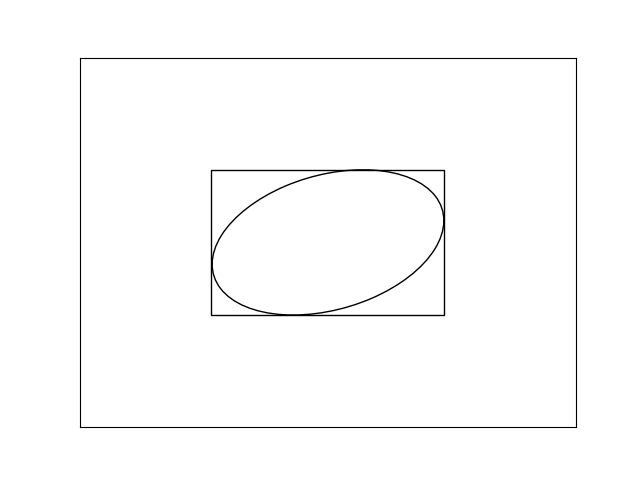
\includegraphics[scale=0.6]{ellipse_bounding_box.png}
        \caption{An ellipse and its bounding box}
        \label{fig:ellipse bounding box}
    \end{figure}
    
    \subsection{Finding Confidence Intervals with \texorpdfstring{\(\chi^2\)}{chisquared}}
    Given \(\chi^2(a, b)\) there are two ways to find a suitable confidence interval.
    The first is to use \(L = \text{const} + Ce^{-\chi^2}\).
    We can then work with maximum likelihoods in a way that is almost identical to with maximum posteriors, for example
    \[\sigma_a^2 = -\left[\pdv[2]{\ln L}{a}\right]^{-1} = \frac{1}{2}\left[\pdv[2]{\chi^2}{a}\right]^{-1},\]
    and similarly for \(\sigma_b^2\) and \(\sigma_{ab}\).
    Alternatively we can generalise the \(\Delta\chi^2\) method used for one-dimensional confidence intervals.
    We first find the value \(\chi^2_{\min} = \chi^2(a_0, b_0)\) and then define \(\Delta\chi^2 = \chi^2 - \chi^2_{\min}\) which will be distributed as \(\chi^2\) with \(\nu = 2\) degrees of freedom.
    It can be shown that we find \SIlist{68.3;90}{\percent} confidence at \(\Delta\chi^2 = \)\SIlist{2.30;4.61}{}.
    We then find the required contour of constant \(\chi^2\).
    
    \subsection{Modelling With Many Parameters}
    The techniques described above generalise fairly easily to \(m\) parameters.
    We can marginalise over any subset of uninteresting parameters and then use one of the methods above to find the confidence interval for the remaining parameters.
    Visualising more than three dimensions at once is hard so it is common to work with two parameters at a time and  look for correlation and then decide based on this how to give the joint errors.
    Assuming that the probability distribution can be approximated as Gaussian we can calculate the covariance matrix
    \[\sigma_{ij} = -\left[\pdvsec{\ln P}{\vartheta_i}{\vartheta_j}\right]^{-1}.\]
    If we find the eigenvalues and eigenvectors of this matrix this gives us the axes of the ellipsoid.
    Let \(\vv{v}\) be a normalised eigenvector of \(\sigma\) with eigenvalue \(\lambda\) then \(\lambda\vv{v}\) is one axis of the ellipsoid.
    We can define a radial distance, \(r = \vartheta_1^2 + \vartheta_2^2 + \dotsb + \vartheta_m^2\), in the \(m\)-dimensional parameter space.
    We can also always perform a transformation of variables such that \(\sigma_{\vartheta_i} = \sigma\) for all \(i\).
    We then simply need to integrate within an \((m-1)\)-sphere\footnote{Note that an \((m-1)\)-sphere is \(S^{m-1}(r) = \{\vv{x}\in\reals^{m}\st \abs{\vv{x}} = r\}\) which is a \((m-1)\)-dimensional surface embedded in \(m\)-dimensional space, for example, \(S^2(1)\) is the unit sphere in three-dimensional space and \(S^1(1)\) is the unit circle in two-dimensional space.} of radius \(r\).
    We then look for which value of \(k = r/\sigma\) we need such that we include the required amount of probability within the surface.
    Generally there is no analytic solution to this problem but numerical solutions do exist.
    As mentioned previously \(\ln L\) and \(\chi^2\) are closely related.
    This means that this problem is equivalent to integrating \(\chi^2\) for \(\nu = m\) degrees of freedom, which we can look up in a table or use numerical methods for.
    We can then use \(\Delta\chi^2 = \chi^2 - \chi^2_{\min}\) which will be distributed as \(\chi^2\) with \(\nu = m\) degrees of freedom.
    The corresponding \(k = r/\sigma\) is then given by \(k = \sqrt{\Delta\chi^2}\).
    The values of \(k\) and \(\Delta\chi^2\) required for common confidence levels is given in table~\ref{tab:multiparameter CI}.
    \begin{table}[ht]
        \centering
        \begin{tabular}{lcccc}\hline\hline
            & \SI{68.3}{\percent} & \SI{90}{\percent} & \SI{95}{\percent} & \SI{99}{\percent}\\\hline\hline
            \(m = 1\) & \(k = 1.00\) & \(k = 1.64\) & \(k = 1.96\) & \(k = 2.58\)\\
            & \(\Delta\chi^2 = 1.00\) & \(\Delta\chi^2 = 2.71\) & \(\Delta\chi^2 = 3.84\) & \(\Delta\chi^2 = 6.63\)\\\hline
            
            \(m = 2\) & \(k = 1.52\) & \(k = 2.15\) & \(k = 2.45\) & \(k = 3.03\)\\
            & \(\Delta\chi^2 = 2.30\) & \(\Delta\chi^2 = 4.61\) & \(\Delta\chi^2 = 5.99\) & \(\Delta\chi^2 = 9.21\)\\\hline
            
            \(m = 3\) & \(k = 1.88\) & \(k = 2.50\) & \(k = 2.95\) & \(k = 3.37\)\\
            & \(\Delta\chi^2 = 3.53\) & \(\Delta\chi^2 = 6.25\) & \(\Delta\chi^2 = 7.81\) & \(\Delta\chi^2 = 11.34\)\\\hline
            
            \(m = 5\) & \(k = 2.43\) & \(k = 3.04\) & \(k = 3.27\) & \(k = 3.85\)\\
            & \(\Delta\chi^2 = 5.89\) & \(\Delta\chi^2 = 9.24\) & \(\Delta\chi^2 = 11.07\) & \(\Delta\chi^2 = 15.09\)\\\hline
            
            \(m = 10\) & \(k = 3.40\) & \(k = 4.00\) & \(k = 4.28\) & \(k = 4.82\)\\
            & \(\Delta\chi^2 = 11.54\) & \(\Delta\chi^2 = 15.99\) & \(\Delta\chi^2 = 18.31\) & \(\Delta\chi^2 = 23.21\)\\\hline
            
            \(m = 20\) & \(k = 4.74\) & \(k = 5.33\) & \(k = 5.60\) & \(k = 6.13\)\\
            & \(\Delta\chi^2 = 22.44\) & \(\Delta\chi^2 = 28.41\) & \(\Delta\chi^2 = 31.41\) & \(\Delta\chi^2 = 37.57\)\\\hline\hline
        \end{tabular}
        \caption{Values of \(k\) and \(\Delta\chi^2\) required to achieve \SIlist{68.3;90;95;99}{\percent} confidence for \(m = 1, 2, 3, 5, 10, 20\).}
        \label{tab:multiparameter CI}
    \end{table}
    \subsection{Goodness of Fit}
    Once we have found the best possible set of parameters how can we see if this model is a good description of the underlying process?
    If we used \(\chi^2\) methods then we can do this fairly easily by performing a one tailed hypothesis that \(\chi^2 \ge \chi^2_{\min}\) where \(\chi^2\) is distributed as \(\chi^2\) with \(\nu = N - m\) degrees of freedom where \(N\) is the number of data points and \(m\) is the number of parameters estimated.
    This relies on an assumption that a Gaussian can be used to model the underlying statistics and we also have to be fairly sure of the errors that we use for each measurement.
    Over estimating errors will lead to overconfidence in the model and underestimating errors can lead to rejecting a model that is actually correct.
    
    If we used Bayesian methods then we cannot get an absolute value of goodness of fit for a model but we can get a relative value to compare to the same model with different parameters.
    We can always calculate \(\chi^2\) with the optimal parameters after using \(P(\vartheta)\) to find these parameters and then using \(\chi^2\) to get an absolute measure of how good the model is.
    If we want to compare two models on the same set of data measured in the same units then we can also compare \(E\) between the two models.
    However this value is sensitive to the units used and the number of data points so if these aren't the same between models then we cannot make this comparison.
    
    \subsection{Model Comparison}
    Suppose we have two models, \(M_1\) and \(M_2\), and we have calculated \(P\) or \(\chi^2\) for both of these.
    First we should test both models to see if they are acceptable.
    Supposing that we fail to reject both models we can still compare them to see which is better.
    
    We can do this using \(\Delta \chi^2\).
    Suppose that \(M_i\) has \(\nu_i\) degrees of freedom and that when compared to the data it gives a best fit \(\chi^2\) value of \(\chi^2_i\).
    Naively we may consider the model with the smaller \(\chi^2_i\) value to be the better model.
    However, there is a chance that this just happened at random.
    Without loss of generality suppose that \(\chi^2_1 > \chi^2_2\).
    We want to come up with some test statistic that we can use for significance testing.
    
    This is possible if the models are \define{nested} meaning that one model is a subset of the other, for example \(M_1\) may be a linear fit and \(M_2\) may be a quadratic, then \(M_1\) is simply \(M_2\) with the \(x^2\) coefficient set to zero.
    In general if we add a parameter we will almost always end up with a lower value of \(\chi^2\) so the question that we have to ask is is the value significantly better.
    The simplest way to test this is using \(\Delta\chi^2 = \chi_1^2 - \chi_2^2\) which, for \(M_1\) being a subset of \(M_2\), is distributed as \(\chi^2\) with \(\nu = \nu_1 - \nu_2\).
    We then use the null hypothesis that both models are equally good and we ask how often we expect \(\Delta\chi^2\) to be this large or larger.
    If we reject the null hypothesis then we can conclude that \(M_2\) is significantly better at whatever confidence level we used.
    This is often called the extra parameter test, i.e. we are testing if it is justified to add another parameter to our model.
    If there is not a significant difference then it is not justified.
    
    Another way to compare models is using the \(F\) statistic defined as
    \[F_{12} = \frac{\chi^2_1/\nu_1}{\chi^2_2/\nu_2} = \frac{\chi^2_1\nu_2}{\chi^2_2\nu_1}.\]
    It can be shown that this is distributed as
    \[P_{\nu_1, \nu_2}(F) = \frac{\Gamma\left(\frac{\nu_1 + \nu_2}{2}\right)}{\Gamma\left(\frac{\nu_1}{2}\right)\Gamma\left(\frac{\nu_2}{2}\right)} \left(\frac{\nu_1}{\nu_2}\right)^{\nu_1/2}F^{\nu_1/2 - 1}\left(1 + \frac{\nu_1}{\nu_2}F\right)^{-(\nu_1+\nu_2)/2}.\]
    This is a two parameter family of curves with mean
    \[\mu_F = \frac{\nu_2}{\nu_2 - 2},\]
    and variance
    \[\sigma_f^2 = \frac{2\nu2^2(\nu_1 + \nu_2 - 2)}{\nu_1(\nu_2 - 2)^2(\nu_2 - 4)}.\]
    As usual we can simply look up pre-calculated values or use numerical methods.
    We have to be careful as \(F_{12} \ne F_{21}\).
    For large \(\nu_1\) and \(\nu_2\) with \(\nu_1 \approx \nu_2 = \nu\) we can approximate this as \(F\distributed\normal(\mu = 1, \sigma^2 = 4/\nu)\).
    
    Another test we can do is the \define{likelihood ratio} test where we compute
    \[R = \frac{L_1}{L_2}\]
    where \(L_i\) is the likelihood of the data given model \(M_i\).
    In general it is possible to find a sampling distribution for \(R\) for any \gls{pdf} that the data follows.
    The most common case being Gaussian.
    In this case if we have \(N\) data points with variance \(\sigma^2\) then we have
    \[\ln L = -\frac{1}{2}N\ln(2\pi\sigma^2) - \frac{\chi^2}{2}.\]
    So comparing the two models likelihoods the only thing that changes between models is \(\chi^2\) so we have
    \[2\ln R = \Delta\chi^2.\]
    So the likelihood ratio test is equivalent to the \(\Delta\chi^2\) test for a Gaussian distribution.
    
    In a similar vain we may compare posterior probabilities using their ratio which, for the case of two fixed hypotheses, is
    \[\frac{P_1}{P_2} = \frac{\pi_1L_1}{\pi_2 L_2}.\]
    So in this simple case of two fixed hypotheses this is simply the likelihood ratio test scaled by the ratio of the priors.
    In a more general case with models \(M_1\) and \(M_2\) we assign priors \(\Pi_1\) and \(\Pi_2\).
    Model \(M_i\) has a parameter vector \(\vartheta_i\).
    The evidence of model \(M_i\) is then
    \[E_i = \int \pi_i(\vartheta_i\st M_i)L_i(D\st \vartheta_i, M_i) \dd{\vartheta_i}.\]
    Note that \(\pi_i(\vartheta_i)\) here is the relative prior probability density for various values of \(\vartheta_i\) in the context of \(M_i\).
    It is not to be confused with \(\Pi_i\) which is the prior for the model \(M_i\) when compared with the other model.
    Similarly \(L_i\) is the likelihood assuming \(M_i\).
    The Bayes factor in this case is then
    \[\frac{P(M_1)}{P(M_2)} = B_{12}\frac{\Pi_1}{\Pi_2}\]
    where \(B_{12} = E_1 / E_2\) is called the \define{Bayes factor}.
    In practice we assume both models are equally likely so \(\Pi_1/\Pi_2 = 1\) and so our relative belief depends only on the Bayes factor.
    
    We can view the Bayes factor, \(B\), as the betting odds on model \(M_1\) vs \(M_2\).
    For example if \(B = 4\) then we say it is \(4:1\) for \(M_1\) and if \(B = 0.2\) then we say it is \(4:1\) against \(M_1\).
    There have also been attempts to turn \(B\) into qualitative words.
    For example, \(B\in [1, 3)\) is `not worth more than a mention', \(B\in [3, 10)\) is `substantial', \(B \in [10, 100)\) is `strong', and \(B > 100\) is `decisive'.
    \clearpage
    \appendix
    \part*{Appendix}
    \addcontentsline{toc}{part}{Appendix}
            \section{Sets and Logic}
        \subsection{Sets}
        A set is a collection of objects, say the objects \(\square\), \(\dagger\), and \(\star\).
        To denote a set containing all of these objects and nothing else we write \(\mathcal{A} = \{\square, \dagger, \star\}\), here `\(\mathcal{A}\)' is just a name that we give the set, in the same way we may say \(x = 2\).
        Sets may contain an infinite number of objects, for example the rational numbers, \(\rationals\), is a set of all fractions of the form \(a/b\) with \(a\) and \(b \ne 0\) being integers.
        The objects in a set are called its elements.
        It is also possible for a set to have no members, in which case we denote this set \(\emptyset\).
        We denote an element being in a set with \(\in\).
        For example we might write \(\square \in \mathcal{A}\) which we read as `\(\square\) is in the set \(\mathcal{A}\)', or \(\pi \in \reals\) which is read as '\(\pi\) is in the set of real numbers' or more commonly as `\(\pi\) is a real number'.
        We denote an element \emph{not} being in a set with \(\notin\), for example \(\diamondsuit \notin \mathcal{A}\) or \(e\notin\rationals\).
        
        Two sets are equal if and only if every element in one set is in the other set and vice versa.
        Note that their is no mention of the order of the elements or how many times an element is included as long as it is included at least one in each set.
        Therefore the following is a true statement:
        \[\mathcal{A} = \{\square, \dagger, \star\} = \{\dagger, \star, \square\} = \{\dagger, \square, \star, \square, \star, \star\}.\]
        Note also that by this definition of equality there is only one empty set, \(\emptyset\).
        It doesn't matter what is not in the set, equality is defined based on what is in the set so if there is nothing in the set then the set is the empty set.
        
        Set builder notation is a way of defining sets where simply listing all of the elements in the set is impractical.
        A set in set builder notation looks like
        \[\mathcal{B} = \{\text{a} \in \mathcal{A} \st \text{condition on }a\}.\]
        Here \(\mathcal{A}\) is some underlying set.
        \(\mathcal{B}\) is composed of elements in \(\mathcal{A}\) such that the given condition on \(a\) is true.
        For example the even numbers could be written as
        \[\{n\in\integers \st n\equiv 0\pmod{2}\}\]
        where \(n \equiv 0 \pmod{2}\) means that \(n/2\) has a remainder of 0.
        
        Two commonly defined operations between set are unions and intersections.
        The union between two sets, \(\mathcal{A}\) and \(\mathcal{B}\) is
        \[\mathcal{A} \union \mathcal{B} = \{a\st a\in\mathcal{A}\;\text{or}\;a\in\mathcal{B}\}.\]
        That is the set of all elements, \(a\), that are in either one of the two sets \(\mathcal{A}\) or \(\mathcal{B}\) (or both sets).
        The intersection between two sets, \(\mathcal{A}\) and \(\mathcal{B}\) is
        \[\mathcal{A} \intersection \mathcal{B} = \{a\st a\in \mathcal{A}\;\text{and}\;\mathcal{B}\}.\]
        That is the set of all elements that are in both of the sets, \(\mathcal{A}\) and \(\mathcal{B}\).
        
        The use of sets in probability is as collections of possible outcomes.
        For example if we are rolling a normal six sided die then the set of all possible outcomes is
        \[\mathcal{S} = {1, 2, 3, 4, 5, 6}\]
        This is the sample space, it is the set of all possible outcomes.
        Suppose we ask the question `what is the chance of rolling an odd prime number'?
        There are two conditions here `odd' and `prime'.
        The set of all odd numbers that are in \(\mathcal{S}\) is
        \[\mathcal{O} = {1, 3, 5}.\]
        The set of all prime numbers in \(\mathcal{S}\) is
        \[\mathcal{P} = {2, 3, 5}.\]
        The set of all odd prime numbers in \(\mathcal{S}\) is then
        \[\mathcal{O} \intersection \mathcal{P} = \{1, 3, 5\} \intersection \{2, 3, 5\} = \{3, 5\}.\]
        Thus we see there are 2 odd primes out of 6 possibilities so the probability of rolling an odd prime is \(2/6 = 1/3\).
        We could ask the similar question `what is the probability of rolling a number that is either odd, prime, or both'?
        The set of all numbers that are odd, prime, or both is
        \[\mathcal{O} \union \mathcal{P} = \{1, 3, 5\} \union \{2, 3, 5\} = \{1, 2, 3, 5\}.\]
        Thus there are 4 numbers that are odd or prime and the chance that rolling the die results in one of these numbers is \(4/6 = 2/3\).
        
        With a frequentist view of probability we see that `and' questions reduce to intersections of sets of possible values whereas `or' questions reduce to unions of sets of possible values.
        This reflects the `and' and `or' in the definitions of intersections and unions.
        
        \subsection{Logic}
        In boolean logic a statement is something that takes one of two values, true, denoted 1, or false, denoted 0.
        We can define various operations on these statements.
        Let \(\mathscr{A}\) and \(\mathscr{B}\) be statements.
        Then we define conjunction, \(\conjunction\), by the following table:
        \[
            \begin{array}{cc|c}
                \mathscr{A} & \mathscr{B} & \mathscr{A} \conjunction \mathscr{B}\\\hline
                1 & 1 & 1\\
                1 & 0 & 0\\
                0 & 1 & 0\\
                0 & 0 & 0
            \end{array}
        \]
        That is \(\mathscr{A}\conjunction\mathscr{B}\) is true only if both \(\mathscr{A}\) and \(\mathscr{B}\) are true.
        We define disjunction, \(\disjunction\), by the following table:
        \[
            \begin{array}{cc|c}
                \mathscr{A} & \mathscr{B} & \mathscr{A} \disjunction \mathscr{B}\\\hline
                1 & 1 & 1\\
                1 & 0 & 1\\
                0 & 1 & 1\\
                0 & 0 & 0
            \end{array}
        \]
        That is \(\mathscr{A}\disjunction\mathscr{B}\) is true so long as at least one of \(\mathscr{A}\) or \(\mathscr{B}\) is true.
        
        We return to rolling a 6 sided die.
        We now use a Bayesian view of probability where we look at confidence in particular statements being true.
        If \(\mathscr{O}\) is the statement `is odd' and \(\mathscr{P}\) is the statement `is prime' then the statement `is odd and prime' is \(\mathscr{O}\conjunction\mathscr{P}\).
        Similarly the statement `is odd or prime' is \(\mathscr{O}\disjunction\mathscr{P}\).
        
        \subsection{Sets and Logic}
        Note the similarity between this notation and the set notation, in particular compare \(\union\)/\(\intersection\) too \(\disjunction\)/\(\conjunction\).
        Also note how the statements \(\mathcal{O}\union\mathcal{P}\)/\(\mathcal{O}\intersection\mathcal{P}\) are the answers too the same questions as \(\mathscr{O}\disjunction\mathscr{P}\)/\(\mathscr{O}\conjunction\mathscr{P}\).
        The reason for this similarity in notation is that (at least when it comes to probability) these two ideas are really equivalent but viewed from a frequentist and Bayesian perspective respectively.
        
        In this work we take both a frequentist and Bayesian view of probability, using whichever better suits our needs.
        For this reason we choose notation that is distinct from both of these.
        If \(A\) and \(B\) are outcomes of some trial then we combine them as
        \[A\logicalAnd B = A, B \iff \mathcal{A} \intersection \mathcal{B} \iff \mathscr{A} \conjunction \mathscr{B},\]
        and
        \[A \logicalOr B \iff \mathcal{A} \union \mathcal{B} \iff \mathscr{A} \disjunction \mathscr{B}.\]
        Here \(\mathcal{A}/\mathcal{B}\) and \(\mathscr{A}/\mathscr{B}\) are the frequentist and Bayesian versions respectively of \(A/B\).
    \section{Size of a Union}
        Suppose that \(A_i\) are sets for some \(i\in {1, \dotsc, n}\).
        Let
        \[\bigunion_{i = 1}^{n} A_i = A_1 \union A_2 \union \dotsb \union A_n = \{a\st a\in A_1\logicalOr A\in A_2\logicalOr\dotsb\logicalOr a\in A_n\}.\]
        It is useful to know what the size of this union is as it often occurs in probability.
        For example
        \[P(A_1\logicalOr A_2\logicalOr \dotsb \logicalOr A_n) = \frac{1}{|S|}\abs{\bigunion_{i = 1}^n A_i}.\]
        We have already seen that in the case \(n = 2\) we have \(|A_1\union A_2| = |A| + |B| - |A\intersection B|\).
        We arrived at this result by counting the elements in each set and then subtracting the elements that we double counted due to them being counted in both sets.
        We can actually be a little bit more rigorous than this with the following theorem\cite[liebeck].
        \begin{theorem}
            Let \(A\) and \(B\) be finite sets.
            Then
            \[|A \union B| = |A| + |B| - |A\intersection B|\]
        \end{theorem}
        \begin{proof}
            Let \(|A\intersection B| = k\).
            Then \(A\union B = \{x_1, \dotsc, x_k\}\).
            These elements, and no others, are in both \(A\) and \(B\) so we have
            \[A = \{x_1, \dotsc, x_k, a_1, \dotsc, a_l\},\qquad\text{and}\qquad B = \{x_1, \dotsc, x_k, b_1, \dotsc, b_m\}\]
            where \(a_i\) and \(b_i\) are all distinct from each other and \(a_i\notin B\) and \(b_i\notin A\) for all \(i\).
            Then clearly \(|A| = k + l\) and \(|B| = k + m\).
            Now we compute the union
            \[A \union B = \{x_1, \dotsc, x_k, a_1, \dotsc, a_l, b_1, \dotsc, b_m\}.\]
            All of these elements are different so
            \begin{align*}
                |A\union B| &= k + l + m\\
                &= (k + l) + (k + m) - k\\
                &= |A| + |B| - |A\intersection B|.
            \end{align*}
        \end{proof}
        That's all well and good for two sets but what about a finite number of finite sets, \(A_i\)?
        We can use another theorem\cite{liebeck}.
        \begin{theorem}
            Let \(n\) be a positive integer, and  let \(A_1, \dotsc, A_n\) be finite sets.
            Then
            \[\abs{\bigunion_{i = 1}^n A_i} = |A_1 \union \dotsb \union A_n| = c_1 - c_2 + c_3 - \dotsb + (-1)^nc_n\]
            where for \(1 \le i \le n\) the number \(c_i\) is the sum of the sizes of the intersections of the sets taken \(i\) at a time.
            For example if \(n = 3\) then
            \begin{align*}
                c_1 &= |A_1| + |A_2| + |A_3|\\
                c_2 &= |A_1 \intersection A_2| + |A_1 \intersection A_3| + |A_2 \intersection A_3|\\
                c_3 &= |A_1 \intersection A_2 \intersection A_3|.
            \end{align*}
        \end{theorem}
        \begin{proof}
            Let \(x \in \bigunion_{i = 1}^n A_i.\)
            We will show that \(x\) contributes exactly once to the expression we have for the size of this union.
            Suppose that \(x\) belongs to precisely \(k\) of the sets \(A_1, \dotsc, A_n\) where \(1 \le k \le n\).
            Then \(x\) contributes \(k\) to the sum 
            \[c_1 = \sum_{1\le i\le n}|A_i|.\]
            \(x\) also contributes to each term of
            \[c_2 = \sum_{1\le i<j \le n}|A_i\intersection A_j|\]
            in which \(A_i\) and \(A_j\) are among the \(k\) sets which contain \(x\).
            There are \({k\choose 2}\) such terms.
            Similarly \(x\) contributes \({k\choose 3}\) to the sum \(c_3\).
            In general \(x\) contributes \({k\choose i}\) to the sum \(c_i\).
            Therefore the total contribution of \(x\) to our expression is
            \[k - {k\choose 2} + {k\choose 3} - \dotsb + (-1)^{k-1}{k\choose k}.\]
            This happens to be 1.
            Hence each element \(x \in A_1\union\dotsb\union A_n\) contributes exactly once to the expression so we find that
            \[\abs{\bigunion_{i = 1}^n A_i} = |A_1 \union \dotsb \union A_n| = c_1 - c_2 + c_3 - \dotsb + (-1)^nc_n.\]
        \end{proof}
    \printbibliography[heading=bibintoc]
\end{document}
